% Options for packages loaded elsewhere
\PassOptionsToPackage{unicode}{hyperref}
\PassOptionsToPackage{hyphens}{url}
%
\documentclass[
  letterpaper,
]{scrbook}

\usepackage{amsmath,amssymb}
\usepackage{lmodern}
\usepackage{iftex}
\ifPDFTeX
  \usepackage[T1]{fontenc}
  \usepackage[utf8]{inputenc}
  \usepackage{textcomp} % provide euro and other symbols
\else % if luatex or xetex
  \usepackage{unicode-math}
  \defaultfontfeatures{Scale=MatchLowercase}
  \defaultfontfeatures[\rmfamily]{Ligatures=TeX,Scale=1}
\fi
% Use upquote if available, for straight quotes in verbatim environments
\IfFileExists{upquote.sty}{\usepackage{upquote}}{}
\IfFileExists{microtype.sty}{% use microtype if available
  \usepackage[]{microtype}
  \UseMicrotypeSet[protrusion]{basicmath} % disable protrusion for tt fonts
}{}
\makeatletter
\@ifundefined{KOMAClassName}{% if non-KOMA class
  \IfFileExists{parskip.sty}{%
    \usepackage{parskip}
  }{% else
    \setlength{\parindent}{0pt}
    \setlength{\parskip}{6pt plus 2pt minus 1pt}}
}{% if KOMA class
  \KOMAoptions{parskip=half}}
\makeatother
\usepackage{xcolor}
\usepackage[normalem]{ulem}
\setlength{\emergencystretch}{3em} % prevent overfull lines
\setcounter{secnumdepth}{5}
% Make \paragraph and \subparagraph free-standing
\ifx\paragraph\undefined\else
  \let\oldparagraph\paragraph
  \renewcommand{\paragraph}[1]{\oldparagraph{#1}\mbox{}}
\fi
\ifx\subparagraph\undefined\else
  \let\oldsubparagraph\subparagraph
  \renewcommand{\subparagraph}[1]{\oldsubparagraph{#1}\mbox{}}
\fi


\providecommand{\tightlist}{%
  \setlength{\itemsep}{0pt}\setlength{\parskip}{0pt}}\usepackage{longtable,booktabs,array}
\usepackage{calc} % for calculating minipage widths
% Correct order of tables after \paragraph or \subparagraph
\usepackage{etoolbox}
\makeatletter
\patchcmd\longtable{\par}{\if@noskipsec\mbox{}\fi\par}{}{}
\makeatother
% Allow footnotes in longtable head/foot
\IfFileExists{footnotehyper.sty}{\usepackage{footnotehyper}}{\usepackage{footnote}}
\makesavenoteenv{longtable}
\usepackage{graphicx}
\makeatletter
\def\maxwidth{\ifdim\Gin@nat@width>\linewidth\linewidth\else\Gin@nat@width\fi}
\def\maxheight{\ifdim\Gin@nat@height>\textheight\textheight\else\Gin@nat@height\fi}
\makeatother
% Scale images if necessary, so that they will not overflow the page
% margins by default, and it is still possible to overwrite the defaults
% using explicit options in \includegraphics[width, height, ...]{}
\setkeys{Gin}{width=\maxwidth,height=\maxheight,keepaspectratio}
% Set default figure placement to htbp
\makeatletter
\def\fps@figure{htbp}
\makeatother
\newlength{\cslhangindent}
\setlength{\cslhangindent}{1.5em}
\newlength{\csllabelwidth}
\setlength{\csllabelwidth}{3em}
\newlength{\cslentryspacingunit} % times entry-spacing
\setlength{\cslentryspacingunit}{\parskip}
\newenvironment{CSLReferences}[2] % #1 hanging-ident, #2 entry spacing
 {% don't indent paragraphs
  \setlength{\parindent}{0pt}
  % turn on hanging indent if param 1 is 1
  \ifodd #1
  \let\oldpar\par
  \def\par{\hangindent=\cslhangindent\oldpar}
  \fi
  % set entry spacing
  \setlength{\parskip}{#2\cslentryspacingunit}
 }%
 {}
\usepackage{calc}
\newcommand{\CSLBlock}[1]{#1\hfill\break}
\newcommand{\CSLLeftMargin}[1]{\parbox[t]{\csllabelwidth}{#1}}
\newcommand{\CSLRightInline}[1]{\parbox[t]{\linewidth - \csllabelwidth}{#1}\break}
\newcommand{\CSLIndent}[1]{\hspace{\cslhangindent}#1}

\usepackage{makeidx}
\makeindex
\makeatletter
\makeatother
\makeatletter
\@ifpackageloaded{bookmark}{}{\usepackage{bookmark}}
\makeatother
\makeatletter
\@ifpackageloaded{caption}{}{\usepackage{caption}}
\AtBeginDocument{%
\ifdefined\contentsname
  \renewcommand*\contentsname{Table of contents}
\else
  \newcommand\contentsname{Table of contents}
\fi
\ifdefined\listfigurename
  \renewcommand*\listfigurename{List of Figures}
\else
  \newcommand\listfigurename{List of Figures}
\fi
\ifdefined\listtablename
  \renewcommand*\listtablename{List of Tables}
\else
  \newcommand\listtablename{List of Tables}
\fi
\ifdefined\figurename
  \renewcommand*\figurename{Figure}
\else
  \newcommand\figurename{Figure}
\fi
\ifdefined\tablename
  \renewcommand*\tablename{Table}
\else
  \newcommand\tablename{Table}
\fi
}
\@ifpackageloaded{float}{}{\usepackage{float}}
\floatstyle{ruled}
\@ifundefined{c@chapter}{\newfloat{codelisting}{h}{lop}}{\newfloat{codelisting}{h}{lop}[chapter]}
\floatname{codelisting}{Listing}
\newcommand*\listoflistings{\listof{codelisting}{List of Listings}}
\makeatother
\makeatletter
\@ifpackageloaded{caption}{}{\usepackage{caption}}
\@ifpackageloaded{subcaption}{}{\usepackage{subcaption}}
\makeatother
\makeatletter
\@ifpackageloaded{tcolorbox}{}{\usepackage[many]{tcolorbox}}
\makeatother
\makeatletter
\@ifundefined{shadecolor}{\definecolor{shadecolor}{rgb}{.97, .97, .97}}
\makeatother
\makeatletter
\makeatother
\ifLuaTeX
  \usepackage{selnolig}  % disable illegal ligatures
\fi
\IfFileExists{bookmark.sty}{\usepackage{bookmark}}{\usepackage{hyperref}}
\IfFileExists{xurl.sty}{\usepackage{xurl}}{} % add URL line breaks if available
\urlstyle{same} % disable monospaced font for URLs
\hypersetup{
  pdftitle={Phonologie der deutschen Sprache},
  pdfauthor={Teodor Petrič},
  hidelinks,
  pdfcreator={LaTeX via pandoc}}

\title{Phonologie der deutschen Sprache}
\usepackage{etoolbox}
\makeatletter
\providecommand{\subtitle}[1]{% add subtitle to \maketitle
  \apptocmd{\@title}{\par {\large #1 \par}}{}{}
}
\makeatother
\subtitle{Im Kontrast mit Slowenisch}
\author{Teodor Petrič}
\date{26.09.22}

\begin{document}
\frontmatter
\maketitle
\ifdefined\Shaded\renewenvironment{Shaded}{\begin{tcolorbox}[enhanced, sharp corners, boxrule=0pt, interior hidden, borderline west={3pt}{0pt}{shadecolor}, breakable, frame hidden]}{\end{tcolorbox}}\fi

\renewcommand*\contentsname{Table of contents}
{
\setcounter{tocdepth}{2}
\tableofcontents
}
\mainmatter
\bookmarksetup{startatroot}

\hypertarget{section}{%
\chapter*{.}\label{section}}
\addcontentsline{toc}{chapter}{.}

\markboth{.}{.}


\includegraphics[width=1\textwidth,height=\textheight]{./pictures/Diapozitiv1.PNG}

\bookmarksetup{startatroot}

\hypertarget{sec-vorwort}{%
\chapter*{Vorwort}\label{sec-vorwort}}
\addcontentsline{toc}{chapter}{Vorwort}

\markboth{Vorwort}{Vorwort}

Dieses Buch ist eine Einführung in die Phonologie der deutschen Sprache,
und zwar unter besonderer Berücksichtigung des Slowenischen im Vergleich
zum Deutschen.

\texttt{Quarto\ Book} \url{https://quarto.org/}

\part{Grundbegriffe und Systematik}

\hypertarget{sec-einfuhrung}{%
\chapter{Einführung}\label{sec-einfuhrung}}

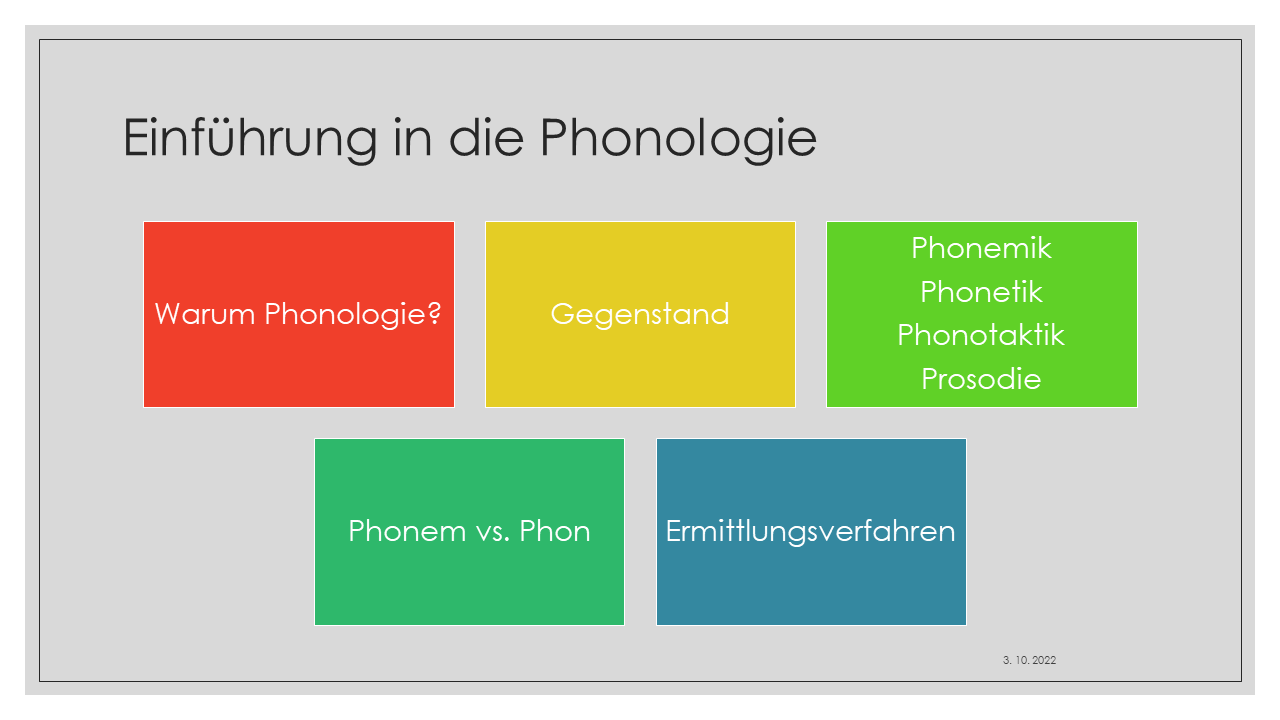
\includegraphics[width=1\textwidth,height=\textheight]{./pictures/Diapozitiv6.PNG}

In diesem Einführungskurs machen wir Sie mit grundlegenden Methoden zur
Erfassung von linguistischen Merkmalen in deutschen (und in einigen
Abschnitten auch mit slowenischen) Texten bekannt.

Diesen Kurs beginnen wir mit Frage, wozu wir überhaupt über Sprache
reden und \emph{zu welchem Zweck über Phonologie?}

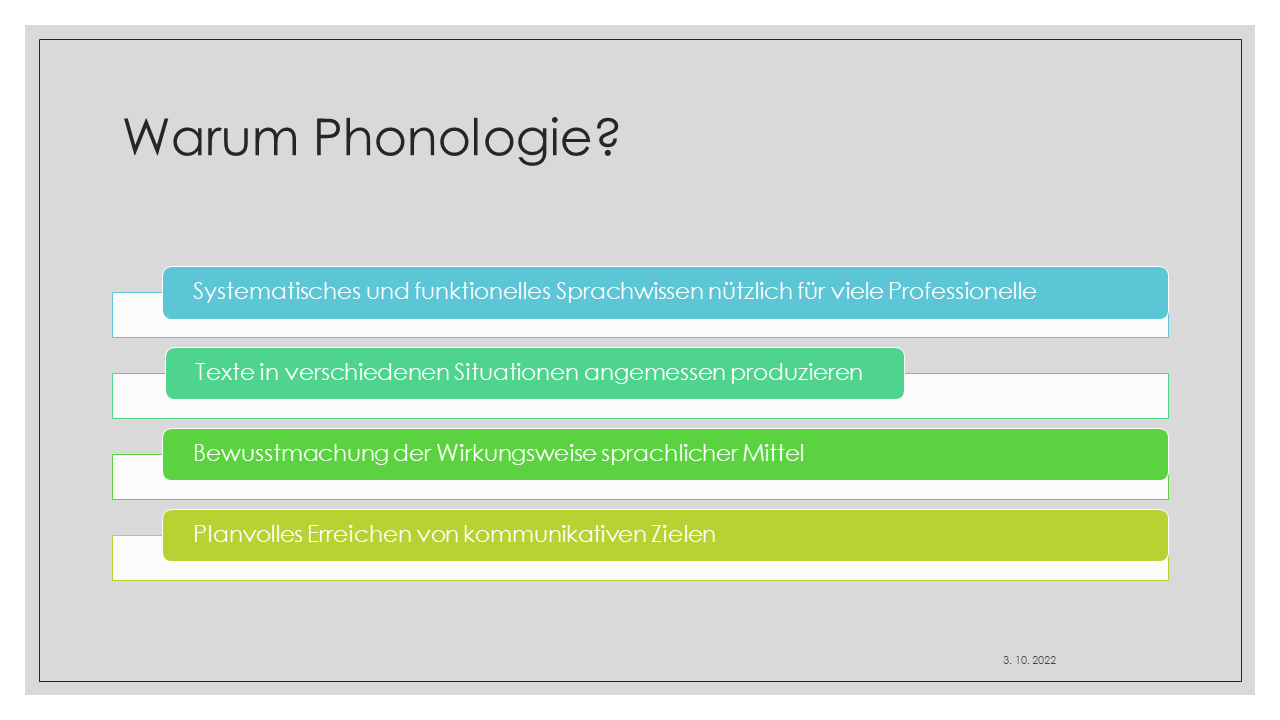
\includegraphics[width=1\textwidth,height=\textheight]{./pictures/Diapozitiv7.PNG}

Da sich mehrere Wissenschaften mit Sprache und folglich auch mit Texten
auseinandersetzen, ist es sinnvoll, Textlinguistik von anderen
wissenschaftlichen Disziplinen abzugrenzen, um den \emph{Gegenstand
\{Chapter~\ref{sec-gegenstand}\} der Phonologie} (als Bestandteil der
Systemlinguistik) besser erkennen zu können.

In jeder wissenschaftlichen Disziplin werden grundlegende Einheiten
definiert. In der Phonologie wird oft das \emph{Phonem} als maßgebliche
Basiseinheit und Ausgangspunkt gewählt. Wie jede linguistische Einheit,
kann man Phoneme verschiedentlich definieren. Andere grundlegende
Einheiten der Phonologie, die in diesem Einführungsbuch definiert,
beschrieben und anhand von exemplarischen Analysen veranschaulicht
werden, sind z.B. \emph{Phon, distinktives Merkmal, Silbe und
Äußerung}.\footnote{Dieses Buch wurde mit \texttt{Quarto}
  \url{https://quarto.org/docs/books/} zusammengestellt.}

Hinweise\footnote{Clipart von \url{https://www.clipartmax.com/}}:

Das ist eine Definition (rmdnote).

Das ist ein Tip oder eine Info (rmdtip).

Das ist ein Arbeitsvorschlag (rmdrobot).

Das ist der RStudio Logotyp (rmdrstudio).

Das ist eine Warnung (rmdwarning).

Das ist eine Fehlermeldung (rmderror).

\hypertarget{sec-gegenstand}{%
\chapter{Gegenstand und Sinn der Phonologie}\label{sec-gegenstand}}

Im Alltag, sei es privat oder im Beruf, verständigen wir uns vorrangig
mit Hilfe von mündlich oder schriftlich geführten Texten. Aufbau und
Wirkung eines Textes sind leichter zu erkennen, wenn man ihn nach
nachvollziehbaren Prinzipien und Methoden in kleinere Einheiten zerlegt.
In der Sprachwissenschaft hat sich eine längere Liste von Einheiten in
Texten etabliert, die man verschiedenen Bereichen zuordnen kann. Hier
sollen vor allem diejenigen Bereiche erwähnt werden, die gemeinsam die
Grammatik einer Sprache umreißen.

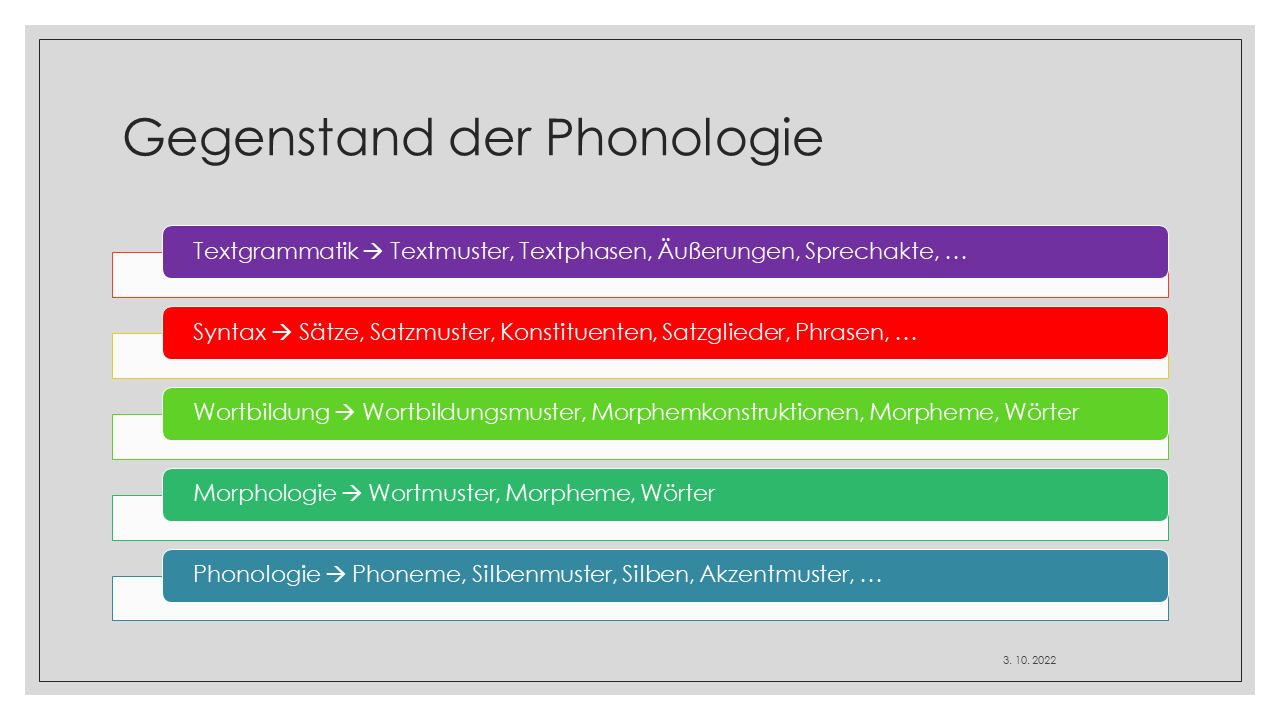
\includegraphics[width=1\textwidth,height=\textheight]{./pictures/Diapozitiv9.PNG}

Der \emph{Text} ist die umfangreichste und hierarchisch höchste
kommunikative Einheit, die aus inhaltlich zusammenhängenden
\emph{Äußerungen} besteht und eine nachvollziehbare und
sortenspezifische Struktur aufweist. (Engel 2008: 33)

\texttt{Äußerungen} lassen sich als Laut- oder Schriftzeichenketten
definieren, die von einem Sprecher zwischen zwei Pausen produziert
werden und aus einem oder mehreren Sätzen bestehen können. (Bußmann
1990: 52) Im Gegensatz zu Sätzen sind sie \texttt{kommunikative}
Einheiten und gehören somit auf die Ebene der \texttt{Performanz} oder
Parole.

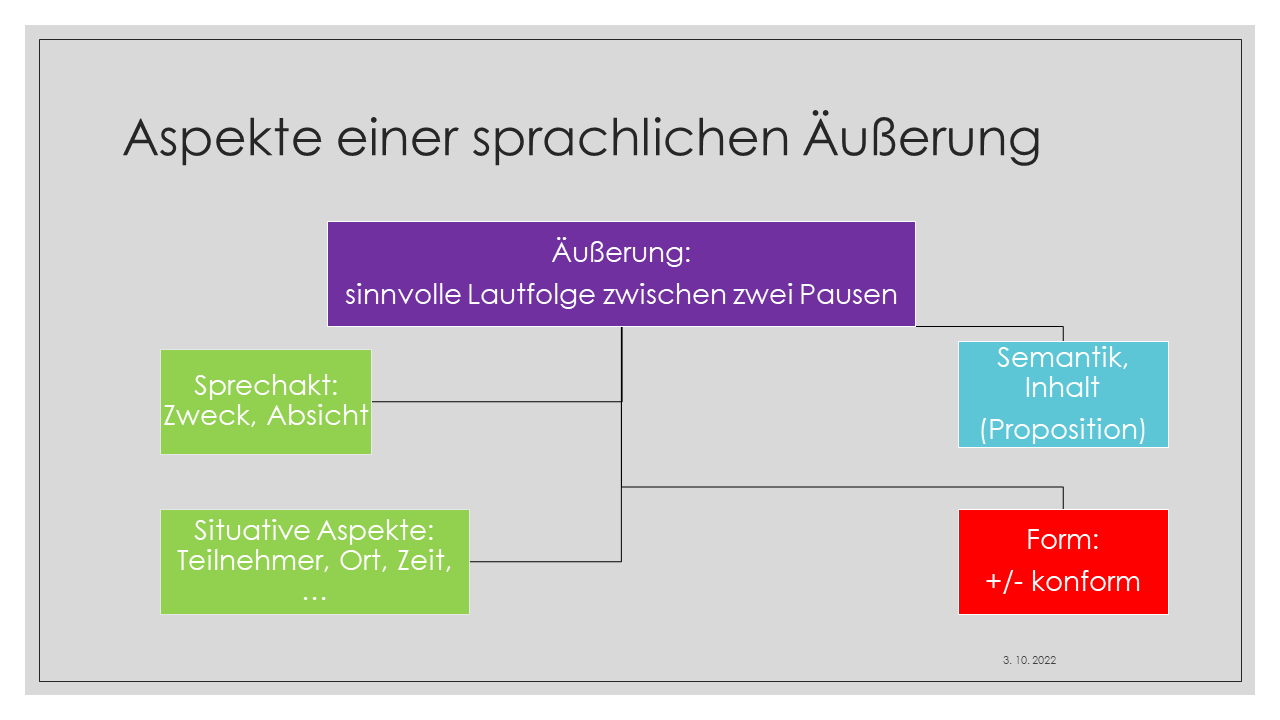
\includegraphics[width=1\textwidth,height=\textheight]{./pictures/Diapozitiv10.PNG}

Die \emph{Phoneme} (distinktive Sprachlauttypen) und \emph{Phone}
(Sprachlaute) gehören zu den kleinsten Einheiten eines mündlichen
Textes.

Die \emph{Phonologie} ist eine Teildisziplin der Sprachwissenschaft, die
sich mit der lautlichen Seite von sprachlichen Äußerungen beschäftigt.
Der Ausdruck wird verschiedenartig verwendet. Im Rahmen dieses
Lehrbuches wird er als Oberbegriff für alle Teildisziplinen verwendet,
die die lautliche Seite von Sprache untersuchen, also als
\emph{Oberbegriff} für \emph{Phonetik}, \emph{Phonemik},
\emph{Phonotaktik} und \emph{Prosodie}. So wird der Ausdruck auch in
amerikanischen sprachwissenschaftlichen Studien verwendet (Bußmann 1990
: 58).

In vielen wissenschaftlichen Arbeiten wird Phonologie im Sinne von
Phonemik verwendet, also in einem eingeschränkteren Sinne als in dieser
Vorlesung. Der slowenische Ausdruck glasoslovje wird von Toporišič
ebenfalls als Oberbegriff für die oben angeführten Teilgebiete verwendet
(vgl. (Toporišič 1992 : 50).

\hypertarget{phonemik-vs.-phonetik}{%
\section{Phonemik vs.~Phonetik}\label{phonemik-vs.-phonetik}}

Die Beschreibung einer Sprache ist aus etischer und emischer Sicht
möglich. Die beiden Wortbildungselemente etisch und emisch bezeichnen
den Unterschied zwischen materieller vs.~funktioneller
Sprachbetrachtung.

\begin{itemize}
\item
  Die \textbf{Phonetik} untersucht die ``akustisch meßbaren und
  artikulatorisch definierbaren aktuellen Lautäußerungen'' (Bußmann
  1983). Sie ``betrachtet Sprache gewissermaßen von außen und erfaßt und
  beschreibt das gesamte vorhandene Lautmaterial, ohne notwendigerweise
  Bezug auf eine bestimmte Sprache zu nehmen.'' (SSM 1: 1). ``Ihre Basis
  sind Erkenntnisse der Anatomie, Physiologie, Neurologie und Physik.''
  (Bußmann 1990 : 579).
\item
  Die \textbf{Phonemik} ``betrachtet die zu beschreibende Sprache von
  innen, d.h. sie untersucht die Beziehung der Laute zueinander und
  deren Funktion in dieser Sprache.
\end{itemize}

Aufgrund der oben getroffenen Unterscheidung zweier Betrachtungsweisen
sind zwei Arten von Grundeinheiten anzusetzen. Definitionen der beiden
Grundeinheiten:

\begin{itemize}
\item
  Als Grundeinheit der Phonetik wird das \textbf{Phon} (der Sprechlaut)
  genannt, d.h. die ``kleinste durch Segmentierung (Zerlegung) gewonnene
  lautliche Einheit, die noch nicht als Repräsentant eines bestimmten
  Phonems klassifiziert ist.'' (Bußmann 1990 : 576).
\item
  Die Grundeinheit der Phonemik ist das \textbf{Phonem}. Das Phonem ist
  ein Lauttyp und wird als Bezeichnung verwendet ``für kleinste aus dem
  Schallstrom der Rede abstrahierte lautliche Segmente mit potentiell
  bedeutungsunterscheidender Funktion.'' (Bußmann 1990 : 576).
\end{itemize}

Die \textbf{Notation} von Phonen bzw. Phonemen unterscheidet sich
voneinander.

\begin{itemize}
\item
  Phone werden in eckigen Klammern notiert: {[}fo:n{]}.
\item
  Phoneme werden hingegen zwischen Schrägstrichen geschrieben: /r/.
\end{itemize}

Die Begriffe Phon und Phonem sollen an einigen Beispielen mit den
stimmlosen bilabialen Verschlußlauten verdeutlicht werden.

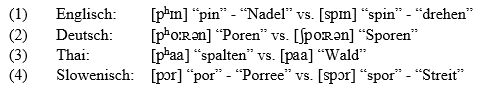
\includegraphics[width=0.6\textwidth,height=\textheight]{./pictures/01b_NSG_Intro_2020-10-07/phoneme_und_allophone1.png}

\begin{itemize}
\item
  \textbf{Aus phonetischer Sicht} kommen in den englischen, deutschen
  und thailändischen Wörtern in (1), (2) und (3) zwei stimmlose
  bilabiale Verschlußlaute vor, und zwar {[}p\textsuperscript{h}{]} und
  {[}p{]}, in den slowenischen in

  \begin{enumerate}
  \def\labelenumi{(\arabic{enumi})}
  \setcounter{enumi}{3}
  \tightlist
  \item
    hingegen nur ein stimmloser bilabialer Verschlußlaut, und zwar
    {[}p{]}. Vom Standpunkt der Phonetik besteht also in dieser Hinsicht
    ein Unterschied zwischen dem Deutschen, Englischen und Thai
    einerseits und dem Slowenischen andererseits.
  \end{enumerate}
\item
  \textbf{Aus phonemischer Sicht} kann man jedoch feststellen, daß die
  Verschlußlaute {[}p\textsuperscript{h}{]} und {[}p{]} im Englischen
  und Deutschen in einem anderen Verhältnis zueinander stehen als im
  Thai. Die beiden Verschlußlaute treten im Englischen und Deutschen in
  unterschiedlichen Umgebungen auf und sind somit ledigliche Varianten
  eines Phonems (\textbf{Allophone}). Im Thai kommen beide
  Verschlußlaute an derselben Stelle im Wort vor. Da ihre lautlichen
  Umgebungen identisch sind, bilden die Laute {[}p\textsuperscript{h}{]}
  und {[}p{]} den einzigen phonetischen Unterschied in diesen Wörtern.
  Die beiden Wörter im Thai haben unterschiedliche Bedeutung, was auf
  die beiden Verschlußlaute zurückgeführt werden kann. Die stimmlosen
  bilabilaen Verschlußlaute {[}p\textsuperscript{h}{]} und {[}p{]} haben
  im Thai bedeutungsunterscheidende Funktion, im Englischen und
  Deutschen hingegen nicht. Daher müssen sie im Thai zwei Phonemen
  zugeordnet werden (6), im Englischen und Deutschen hingegen nur einem
  Phonem (5). Das slowenische Phonem /p/ wird in (4) immer nur durch ein
  Phon realisiert, und zwar durch {[}p{]}.
\end{itemize}

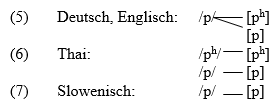
\includegraphics[width=0.3\textwidth,height=\textheight]{./pictures/01b_NSG_Intro_2020-10-07/phoneme_und_allophone2.png}

\hypertarget{phonotaktik}{%
\section{Phonotaktik}\label{phonotaktik}}

Eine weitere wichtige Teildisziplin der Phonologie ist die Phonotaktik.

Die \textbf{Phonotaktik} ist die Lehre von den in einer bestimmten
Sprache zugelassenen Laut- oder Phonemkombinationen. (Bußmann 1990 :
584)

Für jede Sprache kann man phonotaktische Regeln für die Verbindbarkeit
von Phonemen in verschiedenen Stellungen bilden. Im Deutschen und
Slowenischen kann beispielsweise der velare Nasalkonsonant {[}N{]} vor
einem k- auftreten (z.B. dt. \emph{Scha\textbf{n}k}, sl.
\emph{šun\textbf{n}ka}). Andererseits können aber auch Regeln für
Verbindungsbeschränkungen angegeben werden. Der velare Nasalkonsonant
kann weder im Deutschen noch im Slowenischen -- im Unterschied zu
Sprachen in anderen Teilen der Welt (z.B. in Bantusprachen in Afrika) --
am Anfang einer Silbe auftreten (z.B. dt. *{[}N{]}ase, sl. *{[}N{]}oht).
Am Anfang einer Silbe kann jedoch in beiden Sprachen ein
dental-alveolarer Nasalkonsoant erscheinen (z.B. dt. \emph{{[}n{]}ase},
sl. \emph{{[}n{]}oht})

\hypertarget{prosodie}{%
\section{Prosodie}\label{prosodie}}

Eine weitere grundlegende Teildisziplin der Phonologie ist die Prosodie.

Die \textbf{Prosodie} ist die Gesamtheit sprachlicher Eigenschaften wie
Akzent, Intonation, Sprechpausen. (Bußmann 1990 : 618)

Die prosodischen Einheiten beziehen sich im allgemeinen auf Einheiten,
die größer sind als ein \emph{Phonem} (oder \emph{Segment}). Deshalb
werden sie in der phonologischen Literatur auch oft als
\textbf{suprasegmentale} Merkmale bezeichnet. Prosodische oder
suprasegmentale Merkmale beziehen sich demnach auf sprachliche Einheiten
wie z.B. \emph{Silbe}, \emph{Wort} oder \emph{Satz} und \emph{Äußerung}.
Die Prosodie untersucht unter anderem auch \emph{Sprechgeschwindigkeit},
\emph{Grenzsignale (Junkturen)}, \emph{Sprechpausen} und
\emph{Sprechrhythmus}.

\hypertarget{phonem-und-hierarchie}{%
\section{Phonem und Hierarchie}\label{phonem-und-hierarchie}}

Die phonologisch relevanten Einheiten können verschiedenen hierarchisch
gegliederten Ebenen zugeordnet werden. Jede Einheit einer Ebene besteht
aus Einheiten der darunterliegenden Ebene und dient gleichzeitig als
Baustein für die Einheit der nächsthöheren Ebene. Die Anzahl der
phonologisch relevanten Ebenen ist \textbf{theorieabhängig}. Die
\textbf{Phonemebene} wird in phonologischen Modellen oft als die
unterste Ebene der phonologischen Hierarchie angesetzt. Darüber liegen
zumindest die \textbf{Silben- und} die \textbf{Wortebene}. In vielen
Sprachen ist es oft nützlich, auch noch andere Ebenen anzusetzen, etwa
eine \textbf{Akzentgruppenebene}, eine \textbf{Satzebene} und eine
\textbf{Äußerungsebene} anzusetzen, um bestimmte Erscheinungen (wie z.B.
die stellungsbedingte Akzentuierung bestimmter Silben, Frequenzverläufe,
Lautreduktionen, Vokaldauer, u.a.) erklären zu können. Die
Äußerungsebene ist hierarchisch über den anderen Ebenen angesiedelt
(vgl. SSM 1: 3):

\begin{itemize}
\item
  Äußerungsebene
\item
  Akzentgruppe
\item
  Wortebene
\item
  Silbenebene
\item
  Phonemebene
\item
  \ldots{} .
\end{itemize}

~

\hypertarget{phonemik-im-fremdsprachenunterricht}{%
\section{Phonemik im
Fremdsprachenunterricht}\label{phonemik-im-fremdsprachenunterricht}}

Bestimmte Laute kommen in (fast) allen Sprachen der Welt vor, z.B.
bilabiale Verschlußlaute wie {[}p{]} und {[}b{]}, Nasalkonsonanten wie
{[}m{]} (bilabial) und {[}n{]} (dental-alveolar) oder offene Vokale wie
z.B. {[}a{]}.

Allerdings gibt es in jeder Sprache auch bestimmte Laute, die nicht
benutzt werden, obwohl sie theoretisch möglich wären. Stattdessen wird
bekanntlich in jeder eine bestimmte Auswahl getroffen. So gibt es z.B.
im Deutschen oder Slowenischen kein \emph{th} {[}đ{]} wie im Englischen,
im Standardslowenischen kein {[}h{]} und {[}ç{]} wie im Deutschen oder
im Englischen kein {[}x{]} wie im Deutschen.

Oft kommt es vor, dass ein bestimmter Laut im Lautinventar mehrerer
Sprachen angeführt wird, aber die Distribution und/oder Häufigkeit
dieses Lautes kann sich wesentlich unterscheiden (vgl. oben).

Die Phonemik hilft dem Fremdsprachenlernenden, sich des Lautsystems der
eigenen Sprache wie auch des Lautsystems der Fremdsprache bewußt zu
werden. Kennt man nämlich die Unterschiede der beiden Lautsysteme, kann
man eine ganze Reihe von Aussprachefehlern vermeiden und die
Fremdsprache auch schneller und besser erlernen (SSM 1: 4).

Im Deutschen stehen die beiden Frikative {[}x{]} und {[}h{]} in
komplementärer Distribution (d.~h. der glottale Frikativ {[}h{]}
erscheint in nativen Wörtern nur silbeninitial vor Vokal wie
beispielsweise in \textless{}\uline{H}aus\textgreater, {[}x{]} dagegen
in nativen Wörtern nach dem Vokal einer Silbe wie beispielsweise in
\textless na\uline{ch}\textgreater) und können daher nicht zu einem
Phonem zusammengefasst werden.

Der Laryngalkonsonant {[}h{]} steht allerdings in Oppostion zum
Glottisverschlußlaut {[}ʔ{]}, so dass man ausgehend von einem
Minimalpaartest von zwei Phonemen sprechen kann.

Im Standardslowenischen ist {[}h{]} nicht einmal Bestandteil des
Lautinventars. Im Slowenischen besteht somit kein phonemischer
Unterschied zwischen {[}x{]} und {[}h{]}. Daher können beide Laute im
Slowenischen frei miteinander vertauscht werden, ohne dass dadurch ein
Bedeutungsunterschied entsteht. Ein Slowene, der das Phonemsystem seiner
eigenen Sprache und das der deutschen nicht kennt und sich der
unterschiedlichen Funktion der beiden Laute in den beiden Sprachen nicht
bewusst ist, wird große Mühe haben, den Unterschied zwischen {[}x{]} und
{[}h{]} im Deutschen überhaupt wahrzunehmen und den Unterschied in
seiner Aussprache korrekt auszuführen (vgl. SSM 1: 4 zum phonemischen
Wert von {[}r{]} und {[}l{]} im Japanischen und Koreanischen).

\hypertarget{phonemik-und-orthographie}{%
\section{Phonemik und Orthographie}\label{phonemik-und-orthographie}}

Die Phonemik ist notwendig bei der Erarbeitung eines angemessenen
Alphabets. Das \textbf{ideale Alphabet} ist wohl - zumindest vom
Standpunkt eines Schreibers oder Lesers auf einer bestimmten Zeitebene -
\textbf{phonemisch}, d.h. jedem Phonem entspricht ein bestimmtes - und
immer dasselbe - Schriftzeichen (\textbf{Graphem}). In den meisten
Schriftsprachen ist das allerdings nicht der Fall, denn Phoneme und
Grapheme (Buchstaben und Buchstabenverbindungen) sind keineswegs imer
identisch. Die Aussprache von Wortformen in einer Sprache ändert sich
mit der Zeit, während Graphemsysteme solche Veränderungen oft nur
teilweise, überhaupt nicht oder erst nach einer gewissen Zeit mitmachen.
Graphemsysteme richten sich nach mehreren (oft gegensätzlichen)
Gesichtspunkten. Das slowenische Graphemsystem ist zum Beispiel stärker
phonemisch orientiert als etwa das deutsche, englische oder
französische. Im deutschen Graphemsystem spielen morphologisch bedingte
und silbenbedingte Prinzipien eine gewichtigere Rolle als im
slowenischen Graphemsystem.

~

(14)~~~~ Deutsch /i:/~~~~~~~~~~~~~~~ \uline{I}gel~~~~~~~~~~~~~~~~
\textless i\textgreater{}

~~~~~~~~~~~~~~~~~~~~~~~~~~~~~~~~~~~~~~~~~~~~~~
v\uline{ie}l~~~~~~~~~~~~~~~~ \textless ie\textgreater{}

~~~~~~~~~~~~~~~~~~~~~~~~~~~~~~~~~~~~~~~~~~~~~~
\uline{ih}m~~~~~~~~~~~~~~~~ \textless ih\textgreater{}

~~~~~~~~~~~~~~~~~~~~~~~~~~~~~~~~~~~~~~~~~~~~~~
V\uline{ieh}~~~~~~~~~~~~~~~ \textless ieh\textgreater{}

(15)~~~~ Englisch /i/~~~~~~~~~~~~~~~~ m\uline{e}ter~~~~~~~~~~~~~
\textless e\textgreater{}

~~~~~~~~~~~~~~~~~~~~~~~~~~~~~~~~~~~~~~~~~~~~~~
s\uline{ee}~~~~~~~~~~~~~~~~~ \textless ee\textgreater{}

~~~~~~~~~~~~~~~~~~~~~~~~~~~~~~~~~~~~~~~~~~~~~~
s\uline{ea}~~~~~~~~~~~~~~~~~ \textless ea\textgreater{}

~~~~~~~~~~~~~~~~~~~~~~~~~~~~~~~~~~~~~~~~~~~~~~
rec\uline{ei}ve~~~~~~~~~~~ \textless ei\textgreater{}

~~~~~~~~~~~ ~~~~~~~~~~~~~~~~~~~~~~~~~~~~~~~~~~
bel\uline{ie}ve~~~~~~~~~~~ \textless ie\textgreater{}

~~~~~~~~~~~~~~~~~~~~~~~~~~~~~~~~~~~~~~~~~~~~~~ mach\uline{i}ne~~~~~~~~~
\textless i\textgreater{}

(16)~~~~ Französisch /o/~~~~~~~~~~ s\uline{o}t~~~~~~~~~~~~~~~~~~
\textless o\textgreater{}

~~~~~~~~~~~~~~~~~~~~~~~~~~~~~~~~~~~~~~~~~~~~~~
s\uline{au}t~~~~~~~~~~~~~~~~ \textless au\textgreater{}

~~~~~~~~~~~~~~~~~~~~~~~~~~~~~~~~~~~~~~~~~~~~~~
s\uline{eau}~~~~~~~~~~~~~~~ \textless eau\textgreater{}

~~~~~~~~~~~~~~~~~~~~~~~~~~~~~~~~~~~~~~~~~~~~~~
sc\uline{eaux}~~~~~~~~~~~~ \textless eaux\textgreater{}

~

\hypertarget{aufgabenbereich-der-phonetik}{%
\chapter{Aufgabenbereich der
Phonetik}\label{aufgabenbereich-der-phonetik}}

Die Phonetik ist eine Naturwissenschaft auf der Grundlage von Anatomie,
Physiologie, Physik (Akustik) und Mathematik.

Ihre Aufgabe ist nach (Gross 1990 : 35) die materielle Analyse
sprachlicher Äußerungen bzw. Laute als eine der Grundlagen

\begin{itemize}
\item
  der theoretischen Linguistik und Dialektologie und
\item
  für die Lösung praktischer Probleme in der Patholinguistik,
  Sprachdidaktik und Computerlinguistik.
\end{itemize}

Aus dem jeweiligen Ort im Kommunikationsprozeß (Sprecher - Text - Hörer)
ergeben sich laut (Gross 1990 : 36) \textbf{drei Teilgebiete der
Phonetik}:

\begin{itemize}
\item
  Die \textbf{artikulatorische Phonetik} beschreibt die Produktion der
  Laute, und zwar nach Artikulationsart und Artikulationsort.
\item
  Die \textbf{akustische Phonetik} beschreibt die Laute nach ihren
  physikalischen Eigenschaften (z.B. Dauer, Frequenz, Intensität) und
  erstellt mit Hilfe spezieller Meßgeräte verschiedenartige Diagramme
  z.B. Sonagramme.
\item
  Die \textbf{auditive Phonetik} untersucht die Rezeption und Analyse
  sprachlicher Zeichen durch Ohr, Nervenbahnen und Gehirn. Neben rein
  physikalischen Gegebenheiten ist in diesem Teilgebiet immer ein
  gewisses Maß an nicht direkt meßbaren (semantischen, psychologischen)
  Prozessen vorhanden (vgl. (vgl. Neppert and Pétursson 1992 : 8). Die
  auditive Phonetik ist das am wenigsten entwickelte Teilgebiet der
  Phonetik. Jedes Teilgebiet verfügt über eigene Grundeinheiten (vgl.
  Neppert and Pétursson 1992 : 8).
\end{itemize}

Im Rahmen des Phonetikunterrichts für Studenten der Germanistik,
insbesondere Studenten des Deutschen als Fremdsprache, steht der
Teilbereich der artikulatorischen Phonetik meist im Vordergrund, d.h.
die Bildungsweise und der Bildungsort der deutschen Laute.

Durch die Segmentierung von Äußerungen erhält man ein
\textbf{Lautinventar}, d.h. eine Liste aller Laute einer Sprache. Je
genauer man die Untersuchung betreibt, desto länger wird die Liste;
jeder Laut hat nämlich beliebig viele Varianten - in Abhängigkeit von
verschiedenen lautlichen Umgebungen und verschiedenen Sprechern.

Das Lautinventar gilt als Grundlage für den nächsten Schritt, die
Ermittlung von Phonemen (Lautmustern) und des \textbf{Phoneminventars}
einer Sprache. Als Beispiel folgt ein \textbf{Lautinventar der deutschen
Sprache} aus (Gross 1990 : 36-37), das allerdings nicht alle
Lautrealisierungen im Deutschen auflistet.

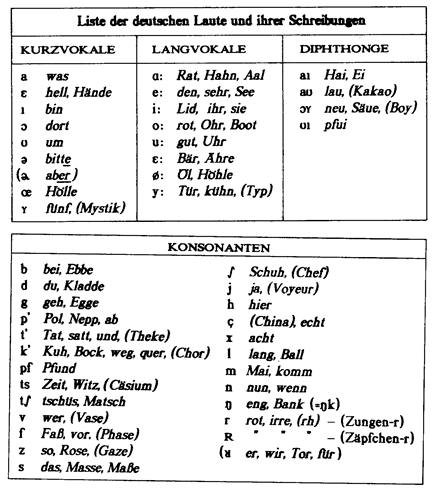
\includegraphics[width=0.6\textwidth,height=\textheight]{./pictures/01b_NSG_Intro_2020-10-07/deutsche_phone.png}

Eine etwas umfangreichere Liste von Lauten der deutschen Sprache finden
sich z.B. in der Dudengrammatik (Grebe and Gipper 1973 : 23-24). Zum
\textbf{slowenischen Laut- und Phoneminventar} vgl. (Toporišič 1992 :
39ff.).

Beantworten Sie einige Fragen zum ersten Kapitel in schriftlicher Form!
(Wiederholung dieser Fragen in mündlicher Form am Anfang des nächsten
Treffens)

\begin{enumerate}
\def\labelenumi{\arabic{enumi}.}
\tightlist
\item
  Welche vier \emph{Teildisziplinen} der Phonologie können wir
  unterscheiden?\\
\item
  Beschreiben Sie in jeweils einem Satz, \emph{wie} sich die einzelne
  Teildisziplin mit der Lautseite der Sprache beschäftigt!\\
\item
  Was unterscheidet \emph{Phone} von \emph{Phonemen}?\\
\item
  Welche Größe hat das \emph{Inventar} deutscher Vokalphoneme im
  Vergleich zum Inventar slowenischer Vokalphoneme? Welches könnte
  deshalb schwerer zu erlernen sein?\\
\end{enumerate}

Lesen Sie das Märchen \emph{Der Bauer und der Teufel} laut vor und
nehmen Sie sich dabei auf (in möglichst guter Klangqualität und ohne
Störgeräusche)! Verwenden Sie für die \emph{Sprachaufnahme} Ihr Handy
oder ein Programm auf Ihrem Computer (z.B. \emph{Praat} oder
\emph{Audacity})! Die Audiodatei soll Ihnen zur Messung von Vokaldauer-
und frequenzwerten mit Hilfe von Praat dienen.

\hypertarget{sprechwerkzeuge-sec-sprechwerkzeuge}{%
\section{Sprechwerkzeuge
{[}\#sec-sprechwerkzeuge{]}}\label{sprechwerkzeuge-sec-sprechwerkzeuge}}

Die Organe, die wir beim Sprechen verwenden (z.B. Lippen, Zunge, Rachen,
Luftröhre, Lungen, Zwerchfell), sind genau genommen nicht speziell fürs
Sprechen entstanden. Die primäre Aufgabe der Lungen, des Zwerchfells und
der Luftröhre ist die Aufnahme von Luft, um den Körper mit dem
notwendigen Sauerstoff zu versorgen. Selbst die Stimmlippen in unserem
Kehlkopf sind nicht speziell für die Sprechtätigkeit entstanden, eher
für viel einfachere Kommunikation (Warnung, Drohung, Abschreckung,
Balzen, \ldots). Auch viele andere Tiere (z.B. Schimpansen, Hunde, Kühe,
Delfine usw.) haben Stimmlippen (Stimmbänder), sind jedoch nicht in der
Lage, so wie Menschen diverse Lautmuster zu komplexer Sprache zu
verwenden. Wenn also in der Phonetik von \emph{Sprechwerkzeugen} die
Rede ist, geht es also um Körperteile und Organe, die sich (evolutionär
betrachtet) \emph{primär} für lebensnotwendige Aufgaben entwickelt haben
und \emph{sekundär} (möglicherweise als evolutionärer Vorteil) aber auch
für komplexe Kommunikationstätigkeiten genutzt werden. Sprache
(Lautsprache) ermöglicht effiziente Übermittlung von Wissen und
wirkungsvolle Zusammenarbeit von Menschen.

Um die Sprechwerkzeuge besser kennen zu lernen, benötigen wir ein wenig
Wissen aus der \emph{Anatomie} des Menschen.

Die erste Abbildung zeigt den \emph{Rachen- und Kehlkopfbereich} im
Sagitallschnitt: den Kehlkopf, den Kehldeckel, die Luftröhre und die
Speiseröhre.

Die zweite und dritte Abbildung zeigen die \emph{Glottis}, in der die
\emph{Stimmlippen} (Stimmbänder) sitzen. Die Stimmlippen ermöglichen die
Erzeugung eines Stimmklangs. Diesen Vorgang nennt man \emph{Phonation}.

Die nächsten Abbildungen zeigen die verschiedenen Glottiseinstellungen
und die daraus resultierenden Sprachlaute.

\begin{figure}

{\centering 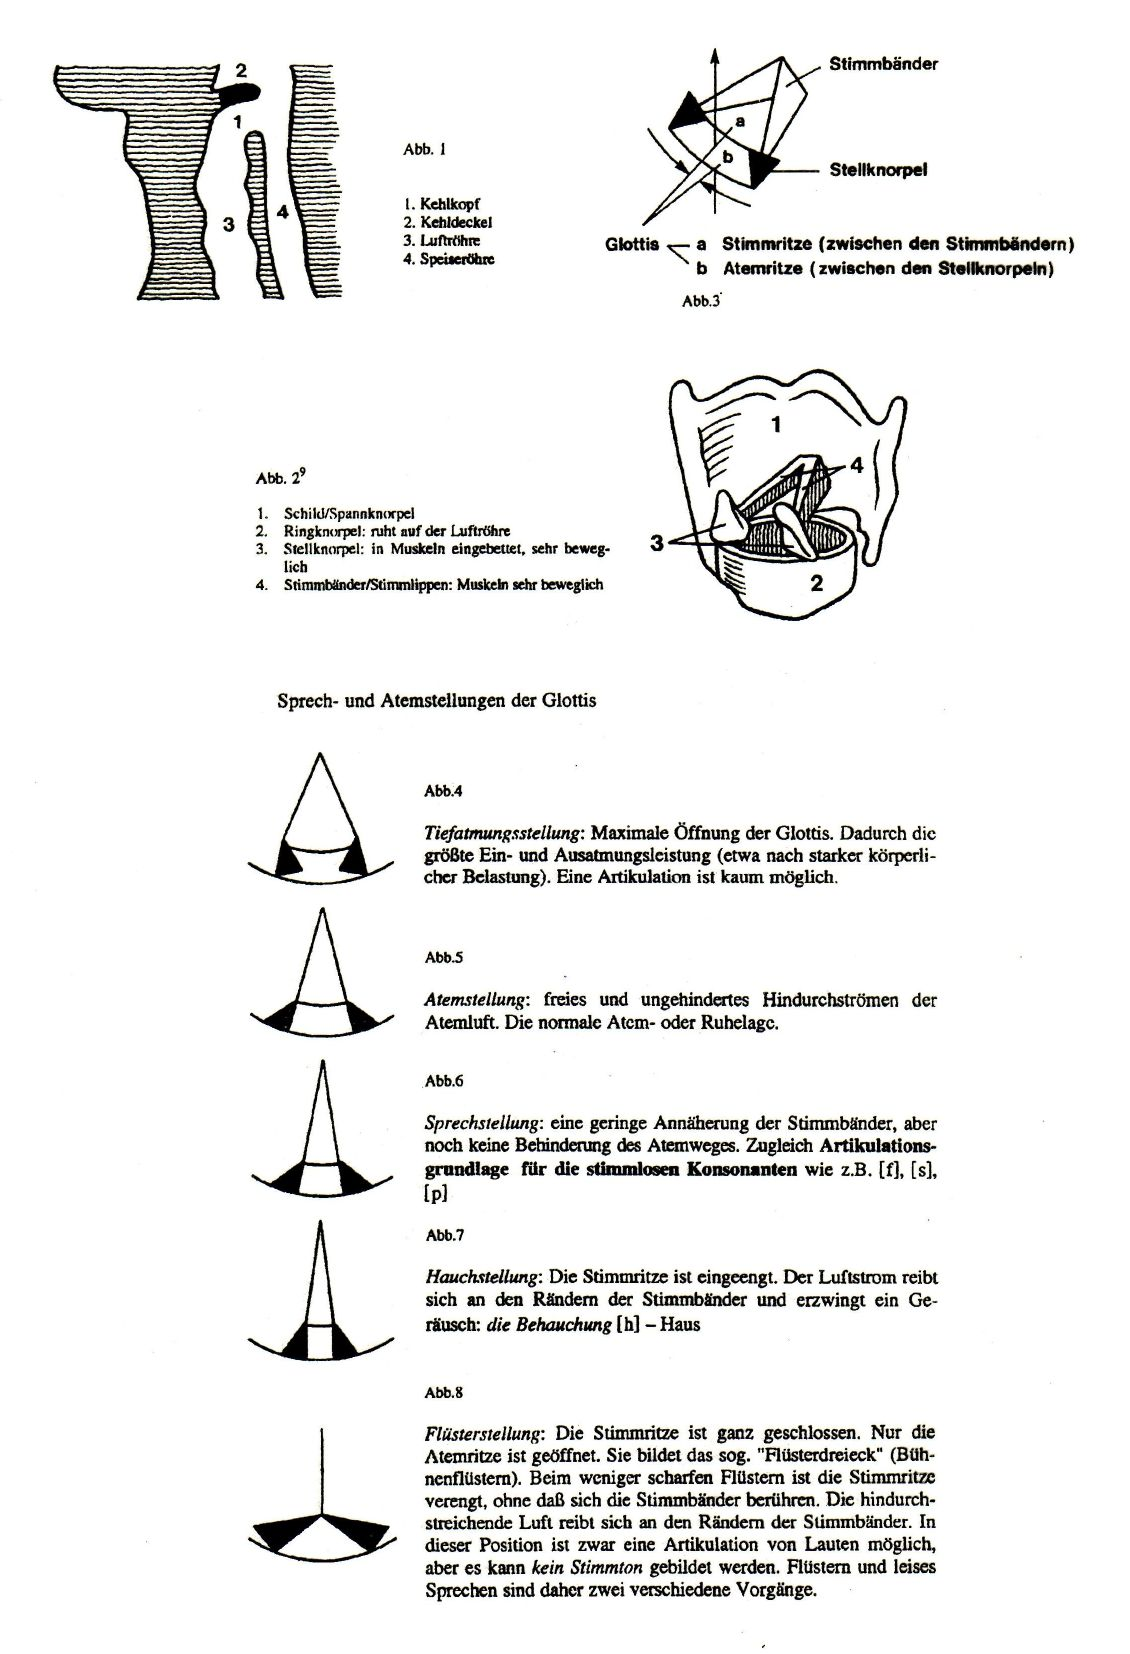
\includegraphics[width=1\textwidth,height=\textheight]{./pictures/02a_Gehrmann-Sprechwerkzeuge_Vokale_page-0001.jpg}

}

\caption{Abbildungen aus Gehrmanns Einführung}

\end{figure}

Glottiseinstellungen: Die Stimmtoneinstellung, notwendig zur Phonation,
und die Verschlussstellung.

Die folgenden Abbildungen zeigen Abbildungen für die Vokale im
Deutschen.

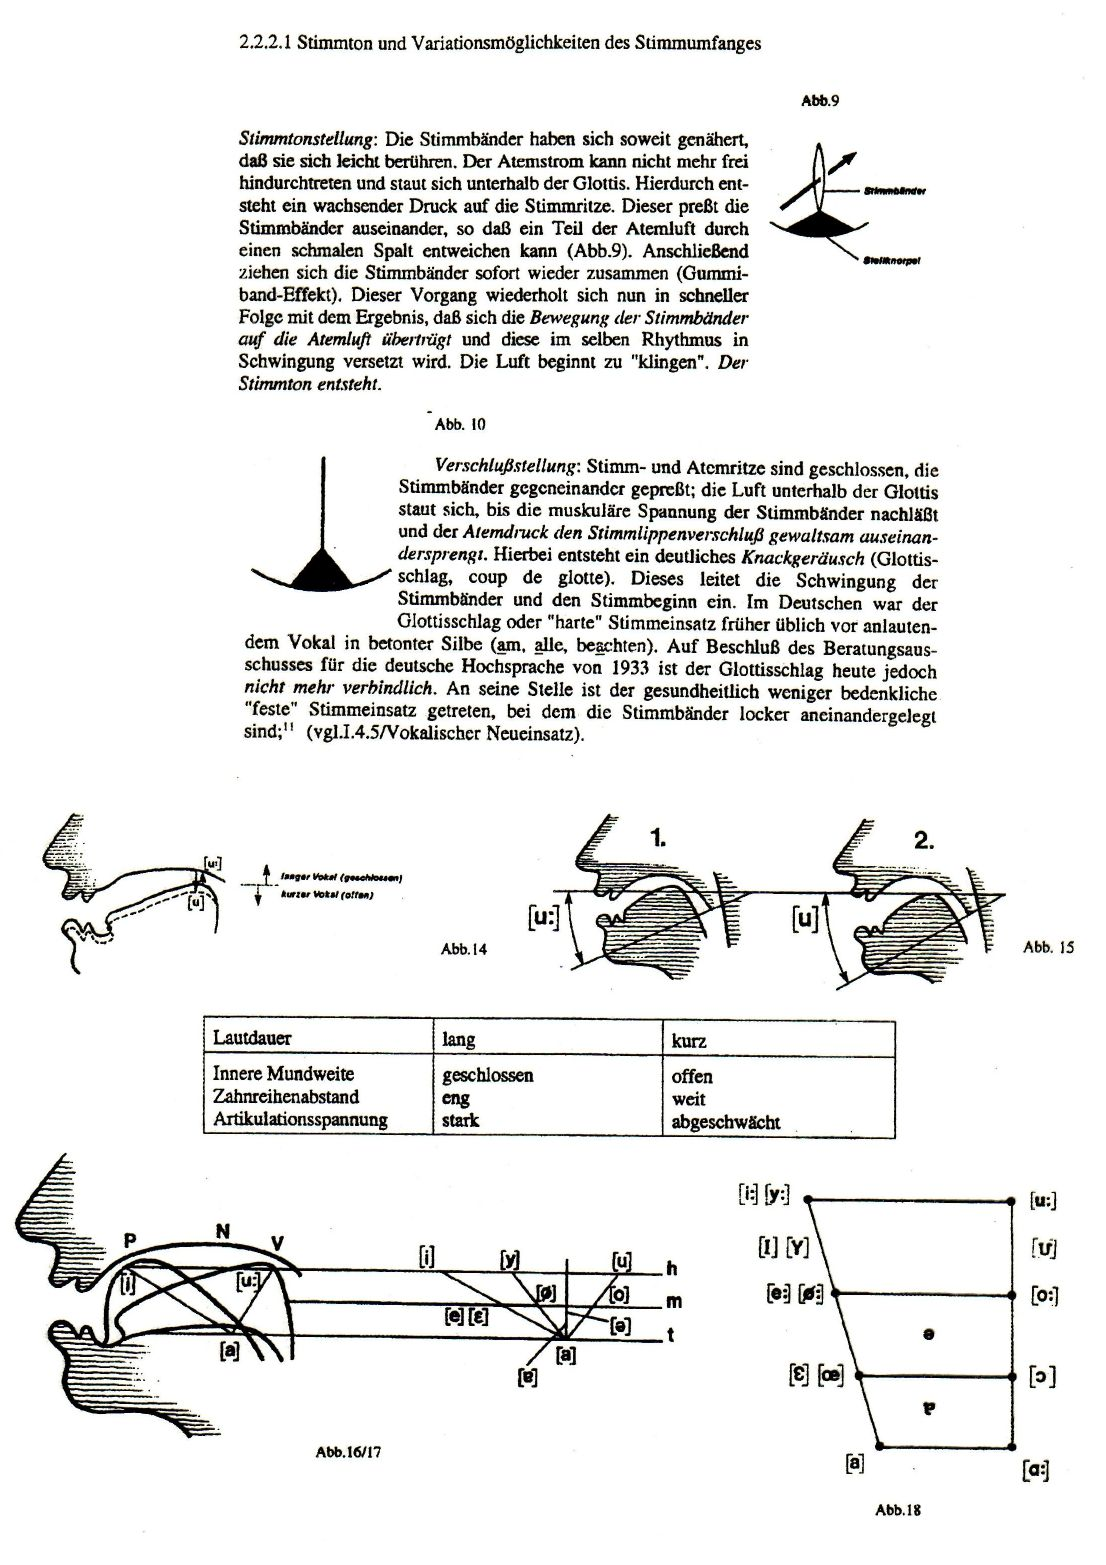
\includegraphics[width=1\textwidth,height=\textheight]{./pictures/02a_Gehrmann-Sprechwerkzeuge_Vokale_page-0002.jpg}

Weitere Abbildungen, mit denen die Bildung deutscher Vokale illustriert
wird.

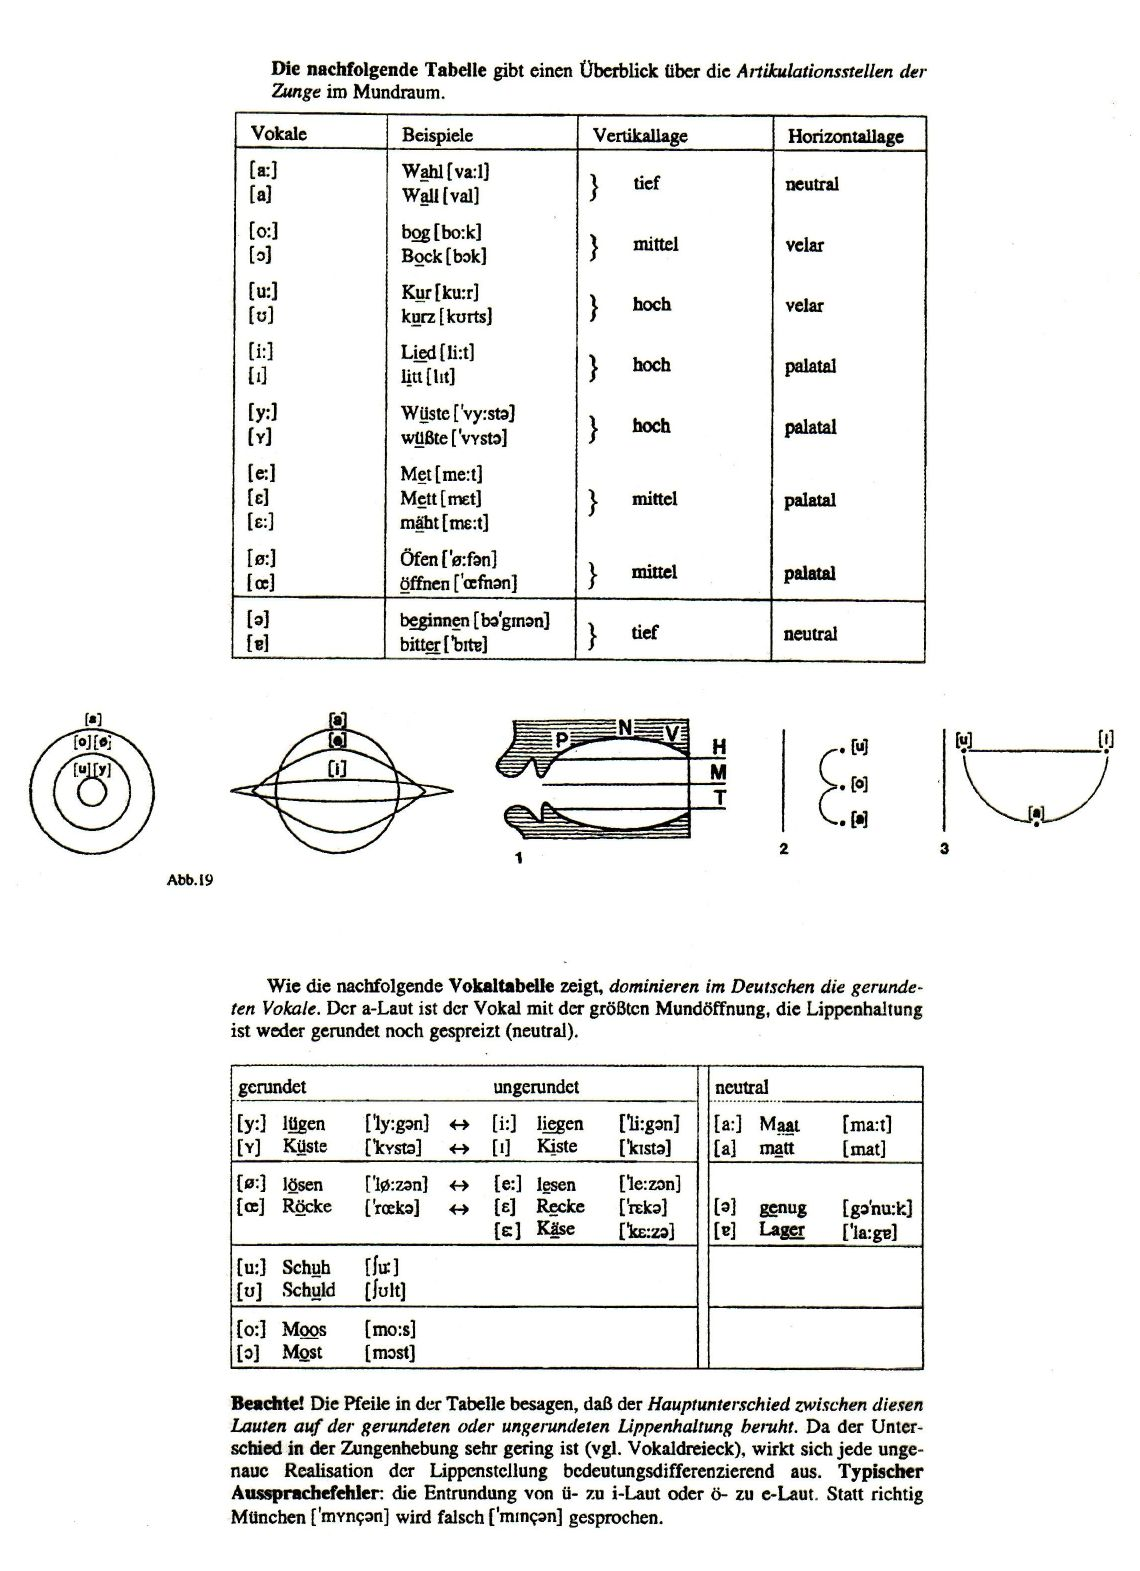
\includegraphics[width=1\textwidth,height=\textheight]{./pictures/02a_Gehrmann-Sprechwerkzeuge_Vokale_page-0003.jpg}

Das Vokaltrapez (Vokalviereck) ist eines der wichtigsten
Abbildungsmittel.

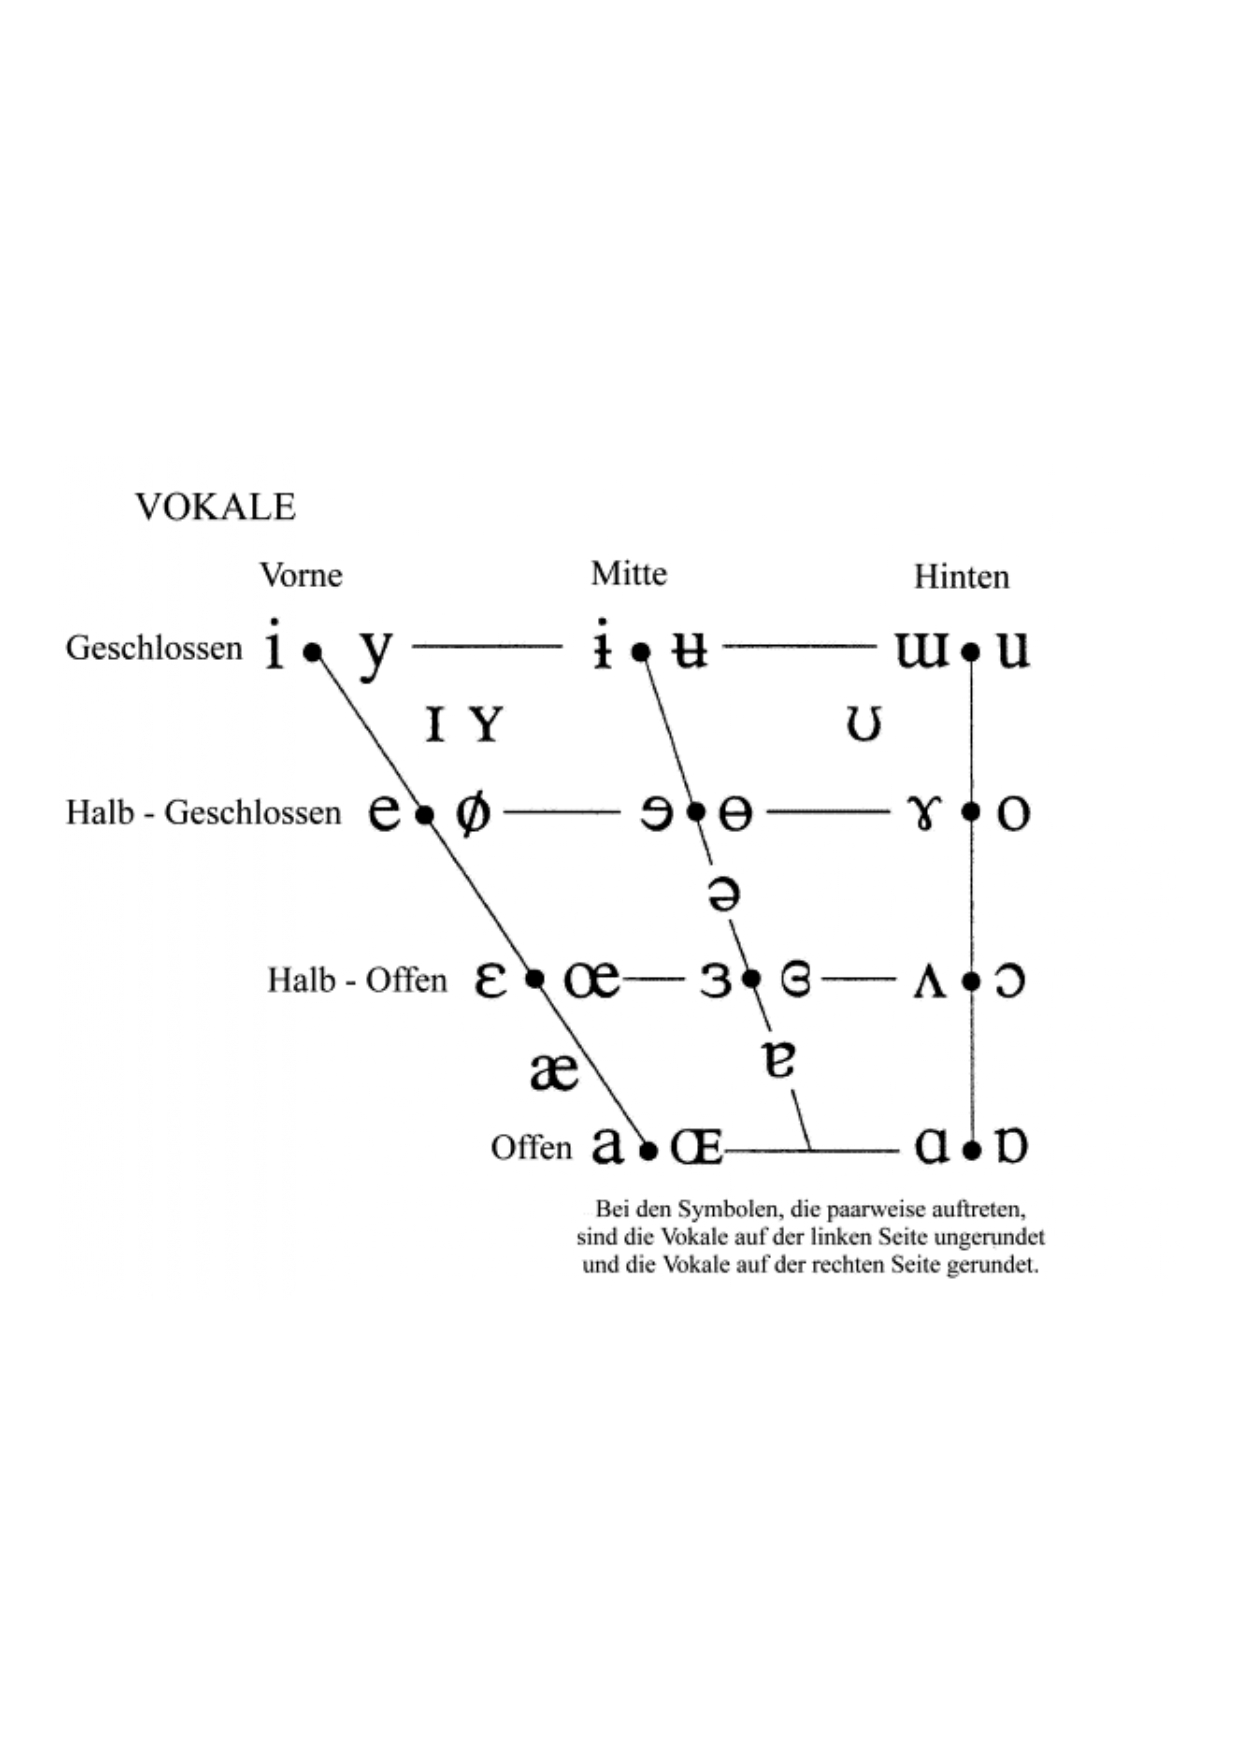
\includegraphics[width=1\textwidth,height=\textheight]{./pictures/02d_vokaltrapez_page-0001.jpg}

Vereinfachte Form des Vokalvierecks.

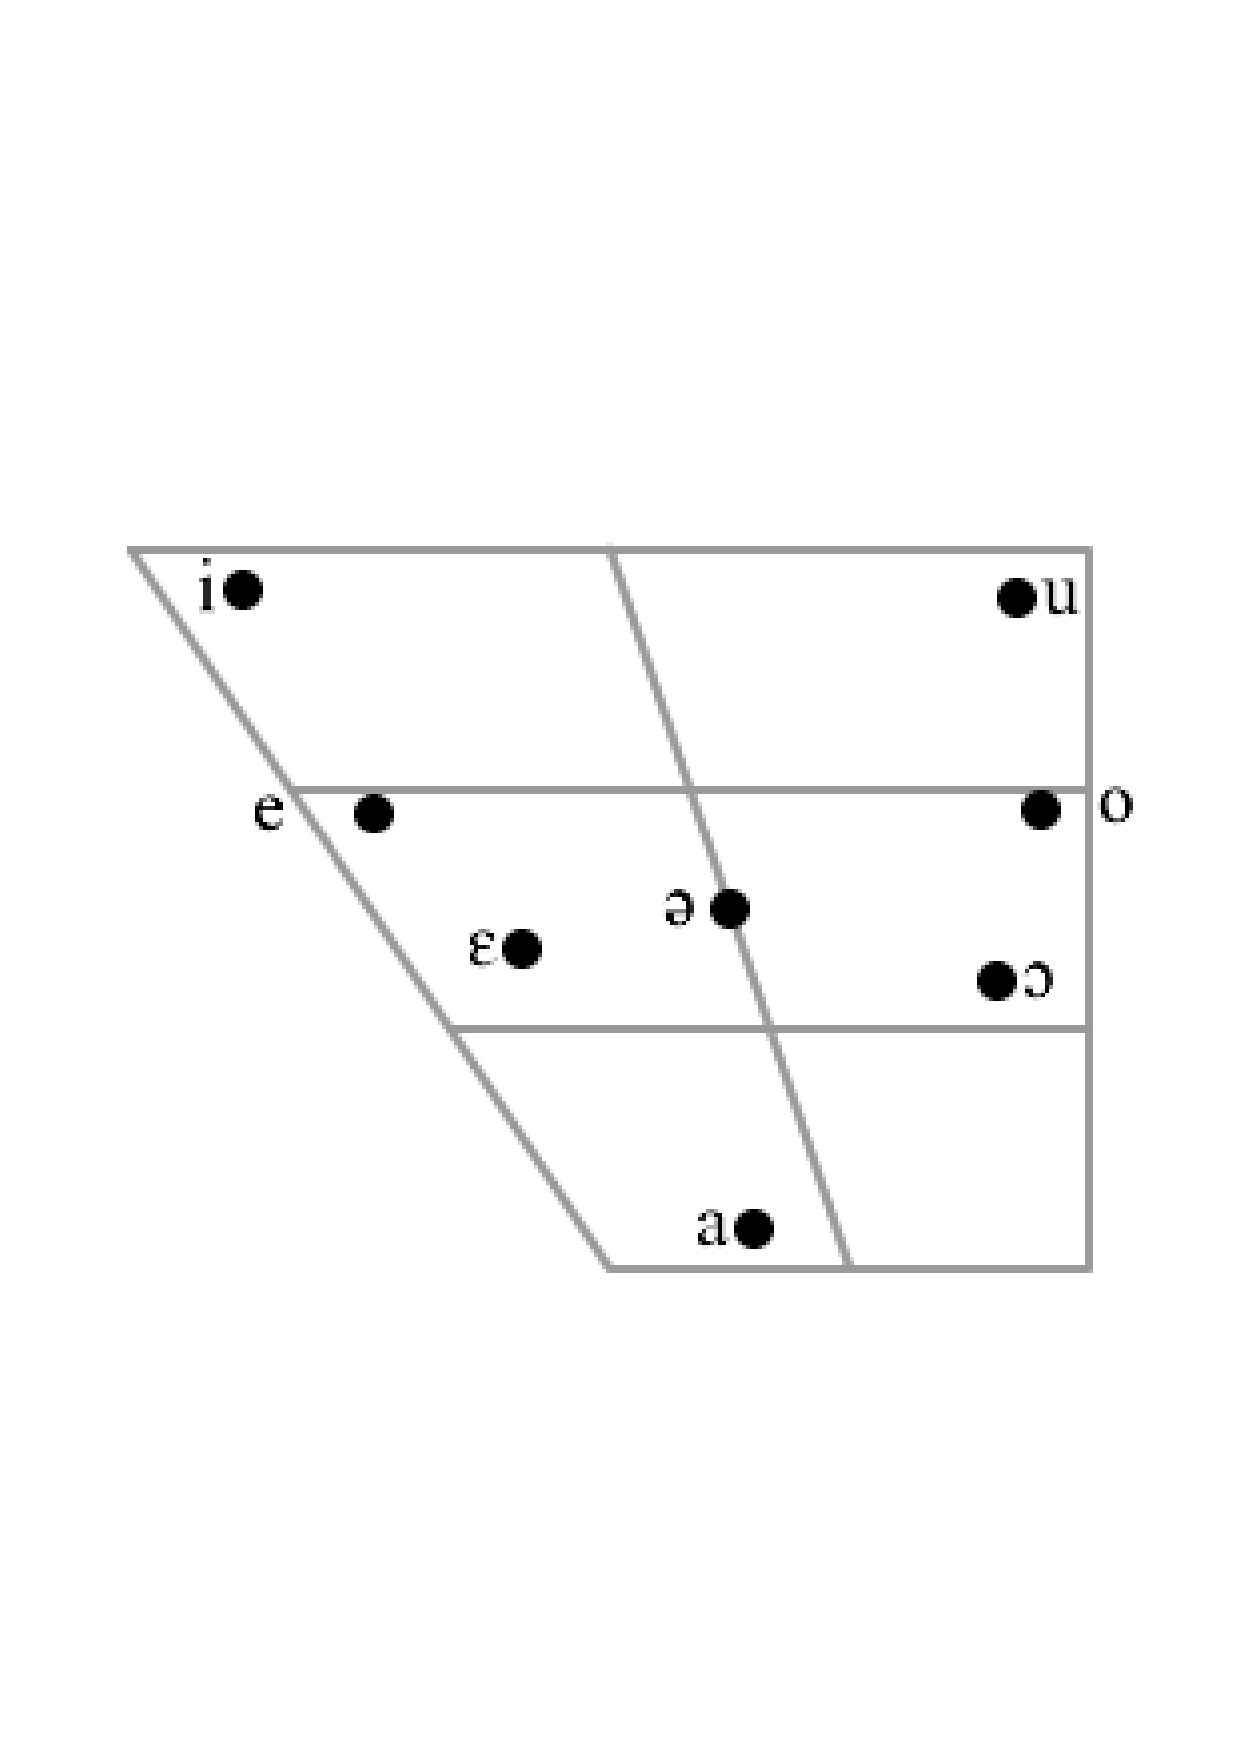
\includegraphics[width=1\textwidth,height=\textheight]{./pictures/02e_Vokaldreieck_Slowenisch_Vowel_chart_Slovenian_page-0001.jpg}

Das Vokalviereck in 3-dimensionaler Version (mit zusätzlicher
Informationen über die Lippenform).

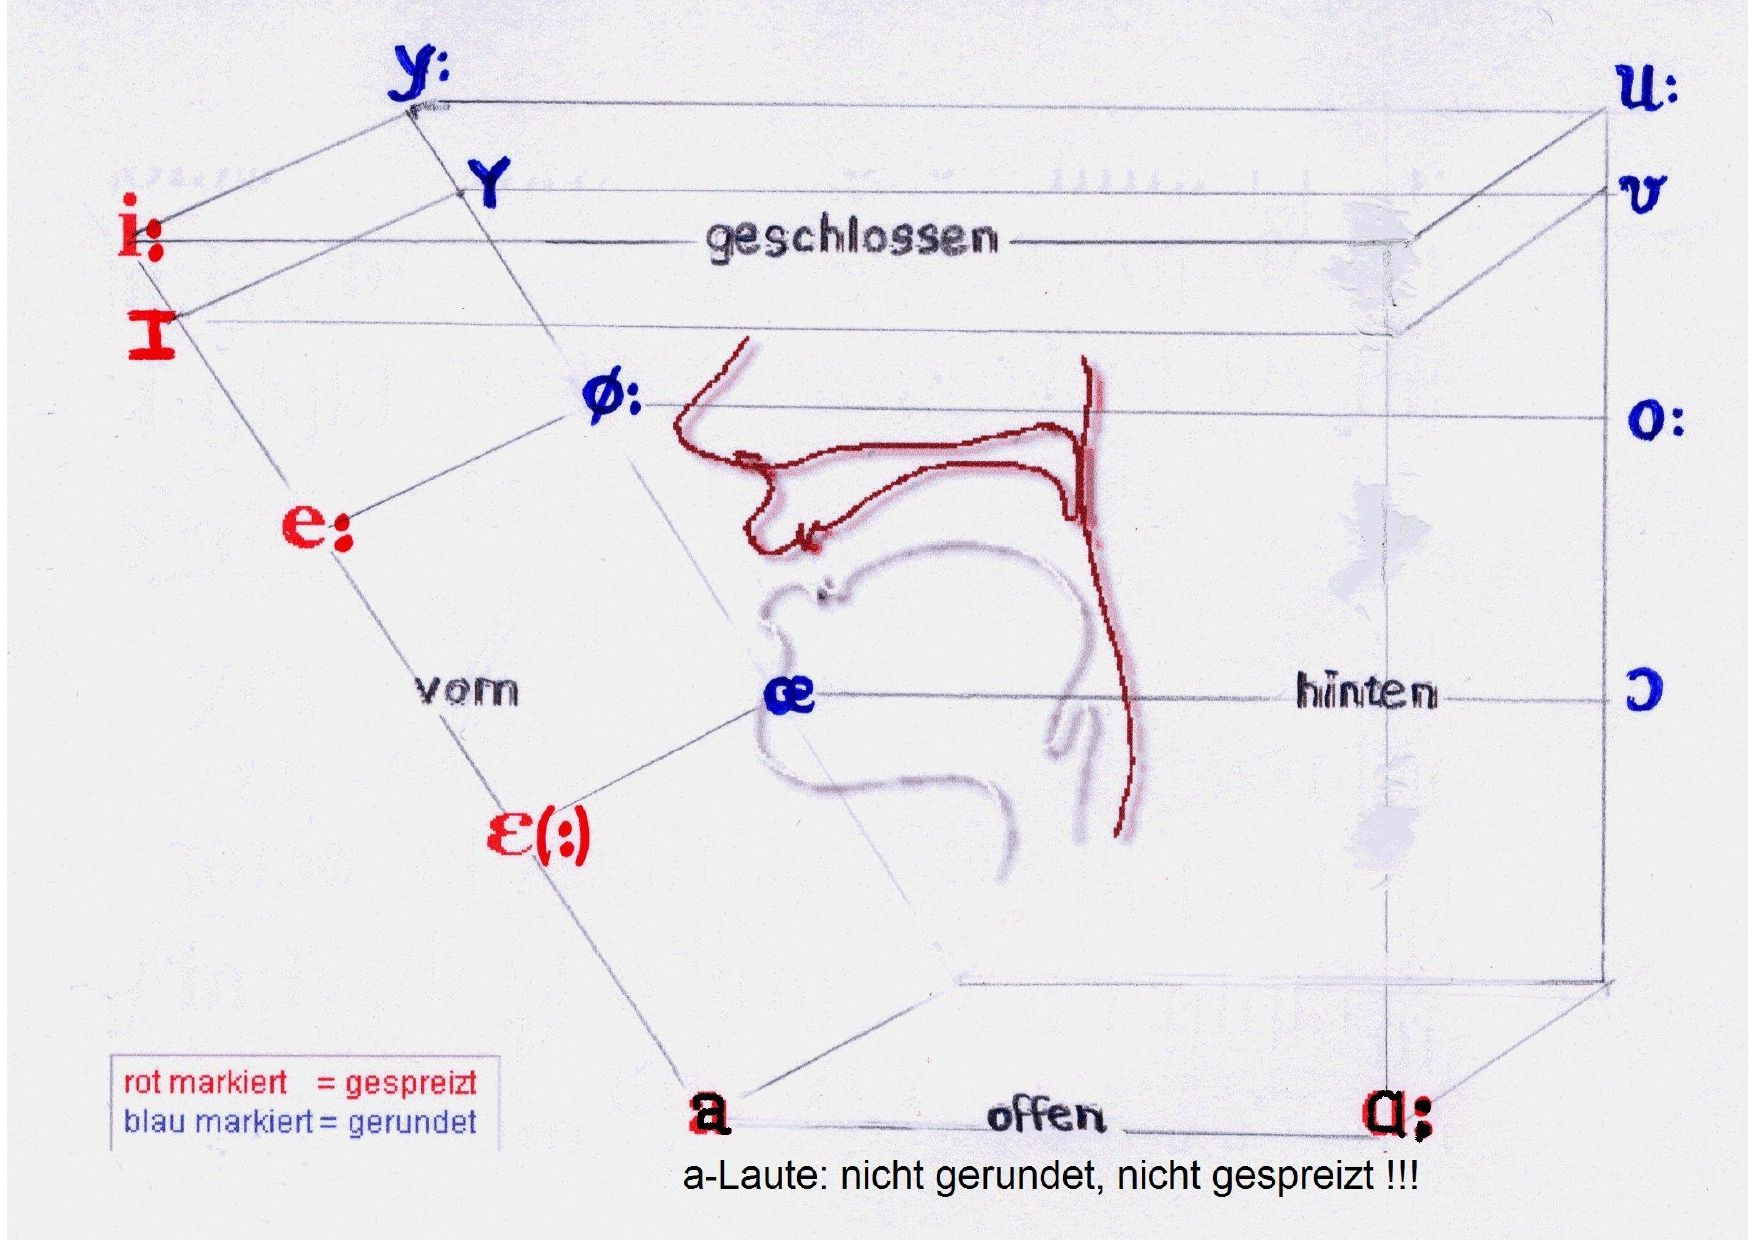
\includegraphics[width=1\textwidth,height=\textheight]{./pictures/02e_Vokale_3D_Deutsch_page-0001.jpg}

Abbildungen aus Wanglers Phonetik-Atlas: Sprechwerkzeuge und
Vokaltrapez.

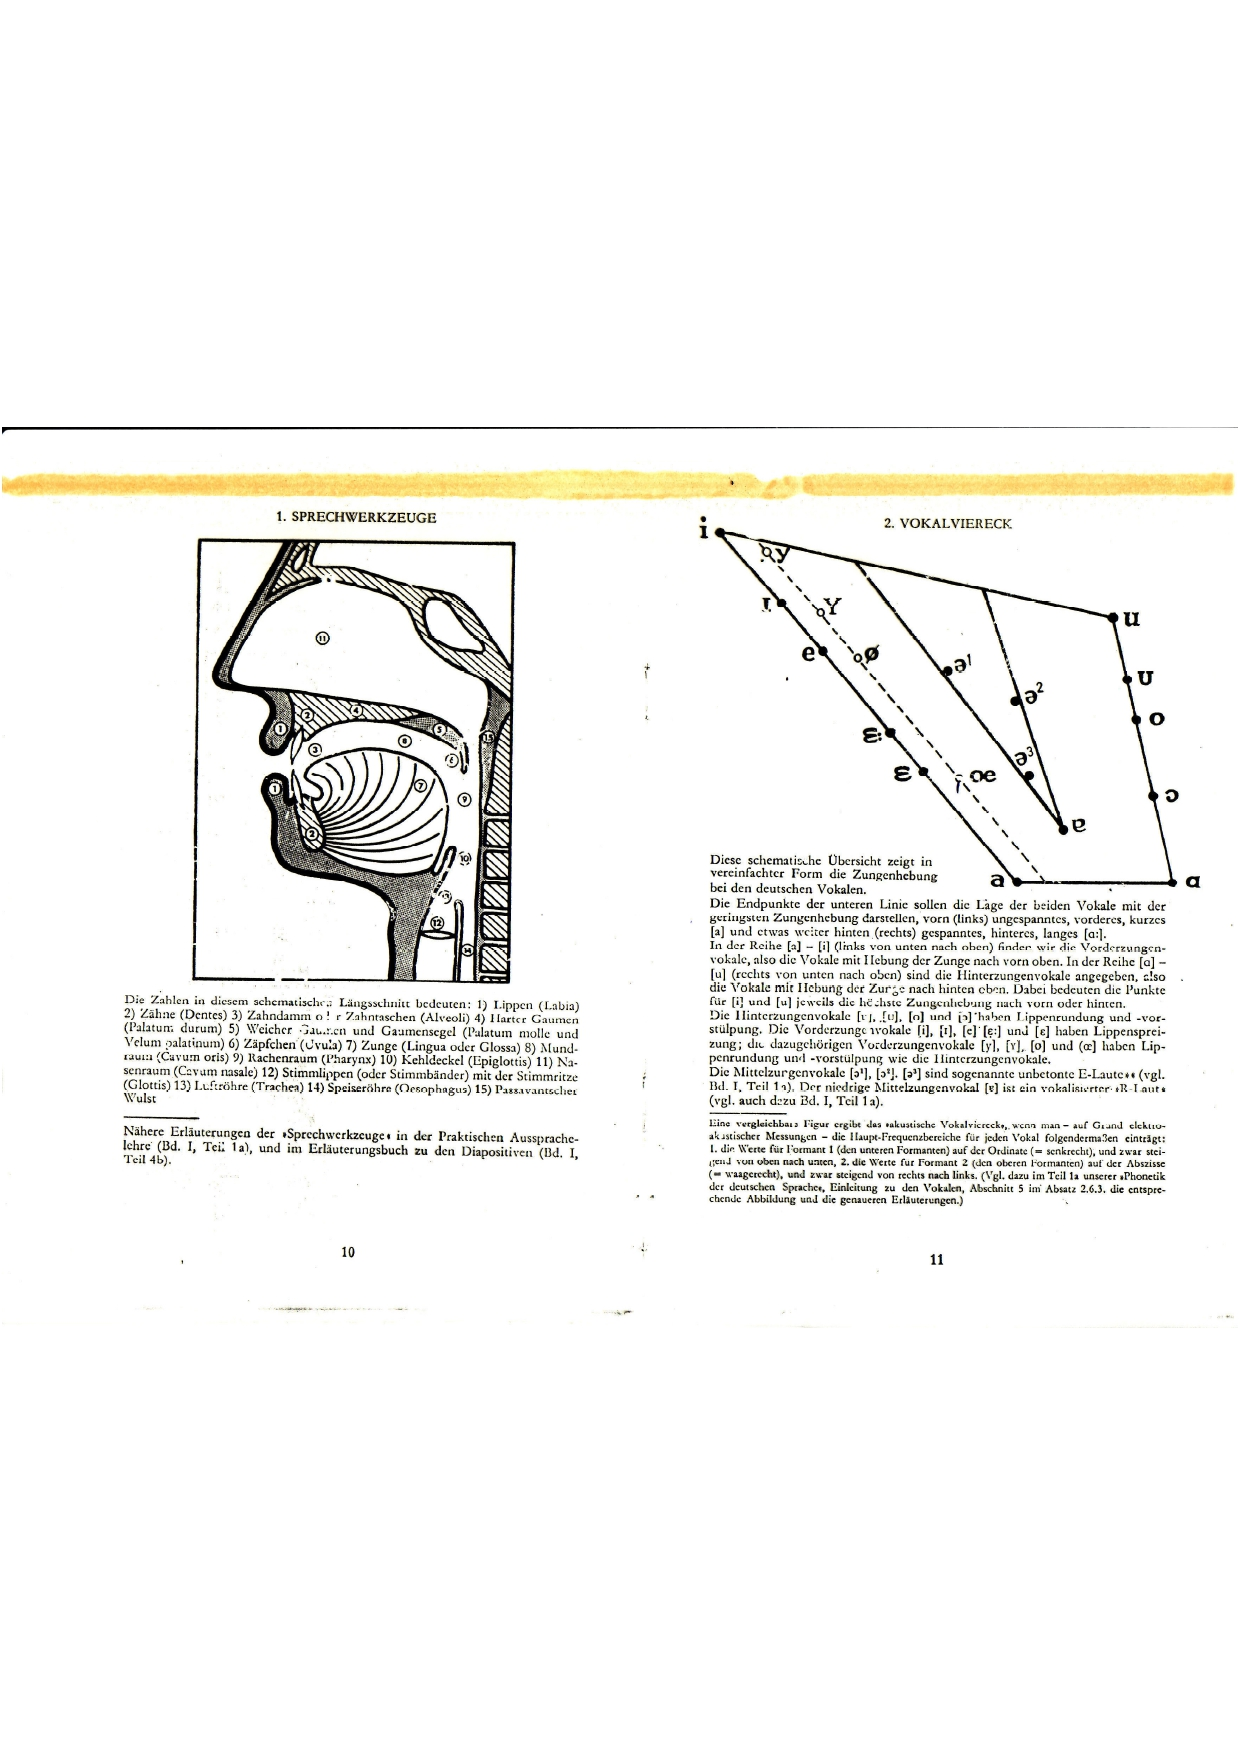
\includegraphics[width=1\textwidth,height=\textheight]{./pictures/02f_Phon-Atlas-Seiten1-2_Diphthonge_page-0001.jpg}

Diphthonge (vokalische Zwielaute) im Deutschen und andere Abbildungen,
typisch für die Beschreibung der Vokalbildung (Wangler).

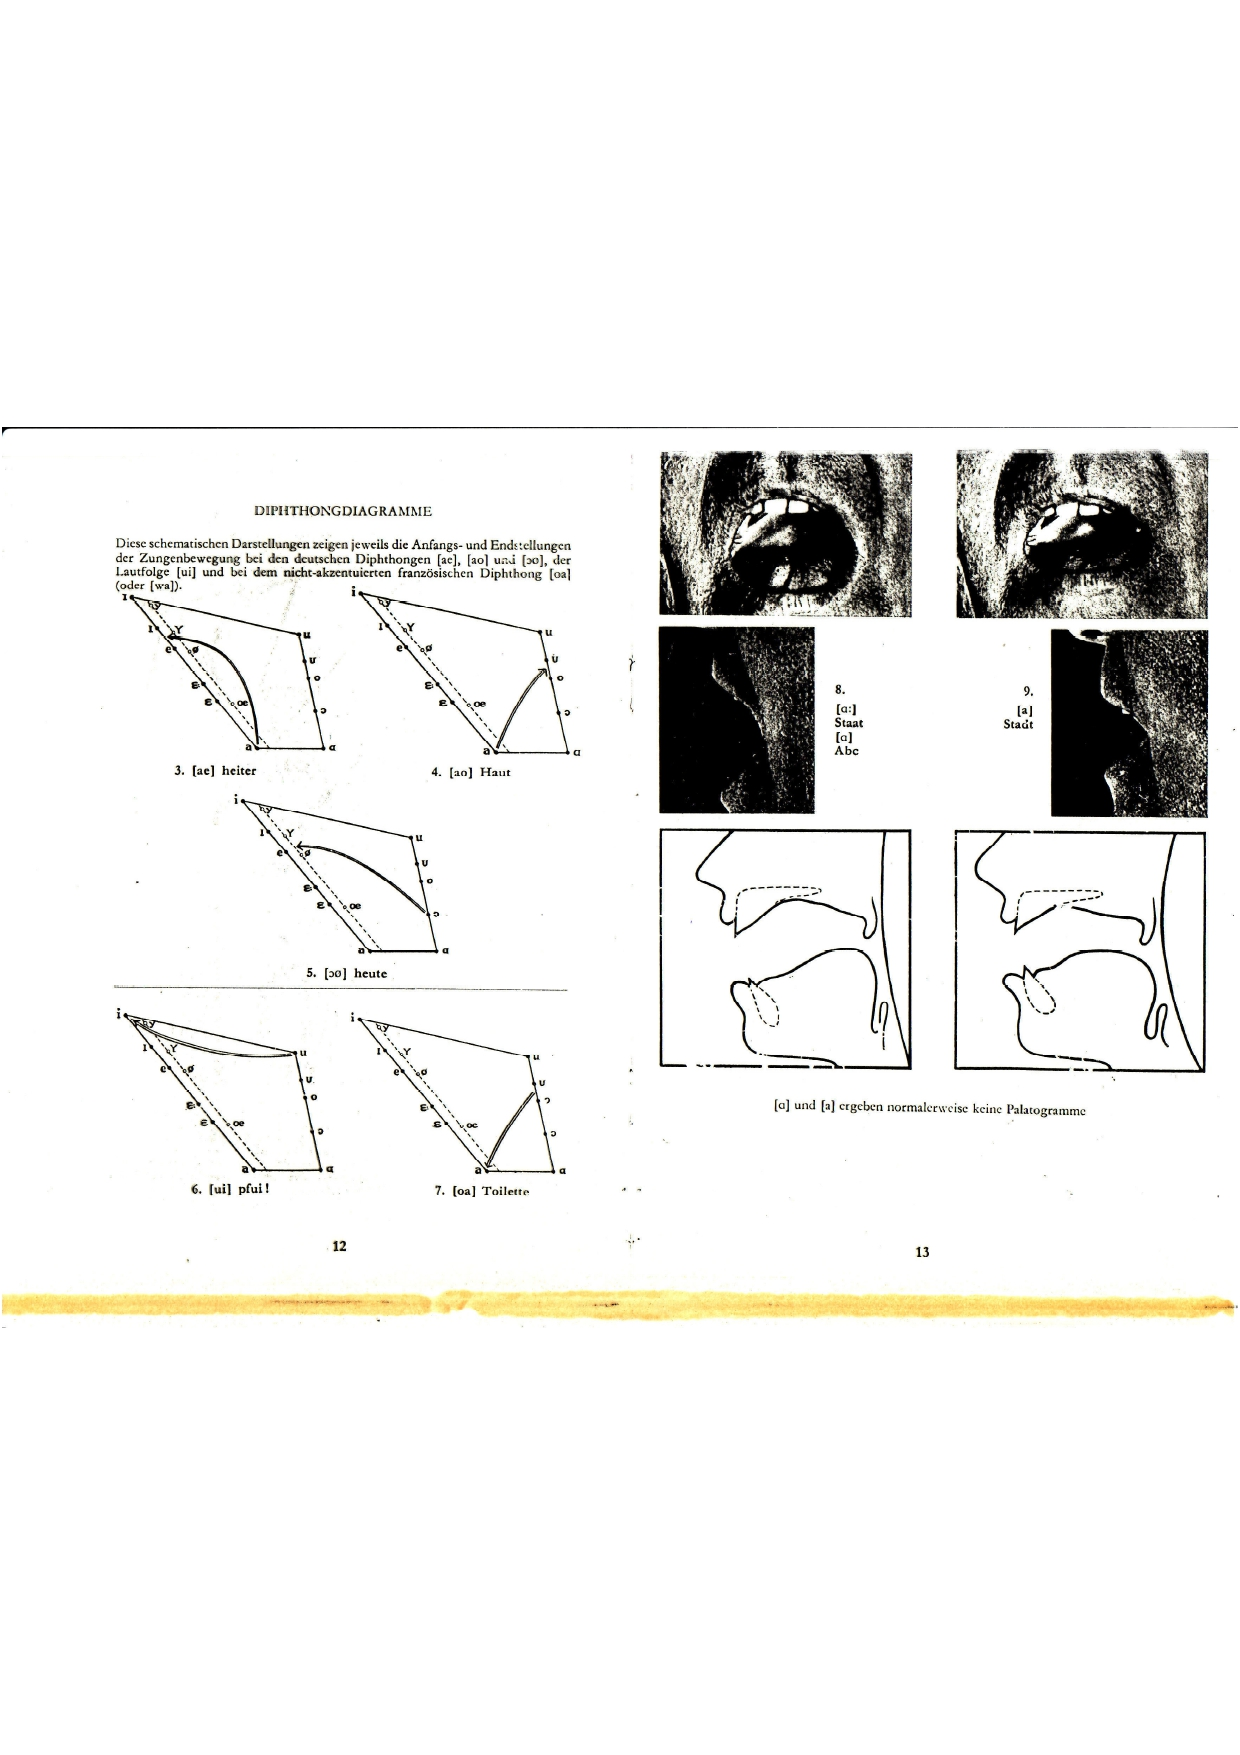
\includegraphics[width=1\textwidth,height=\textheight]{./pictures/02f_Phon-Atlas-Seiten1-2_Diphthonge_page-0002.jpg}

Eine Tabelle, in der die Bildung deutscher Konsonanten systematisch
abgebildet ist, und zwar nach drei Gesichtspunkten: Artikulationsorgan,
Artikulationsstelle, Artikulationsmodus und Stimmtonaktivierung.

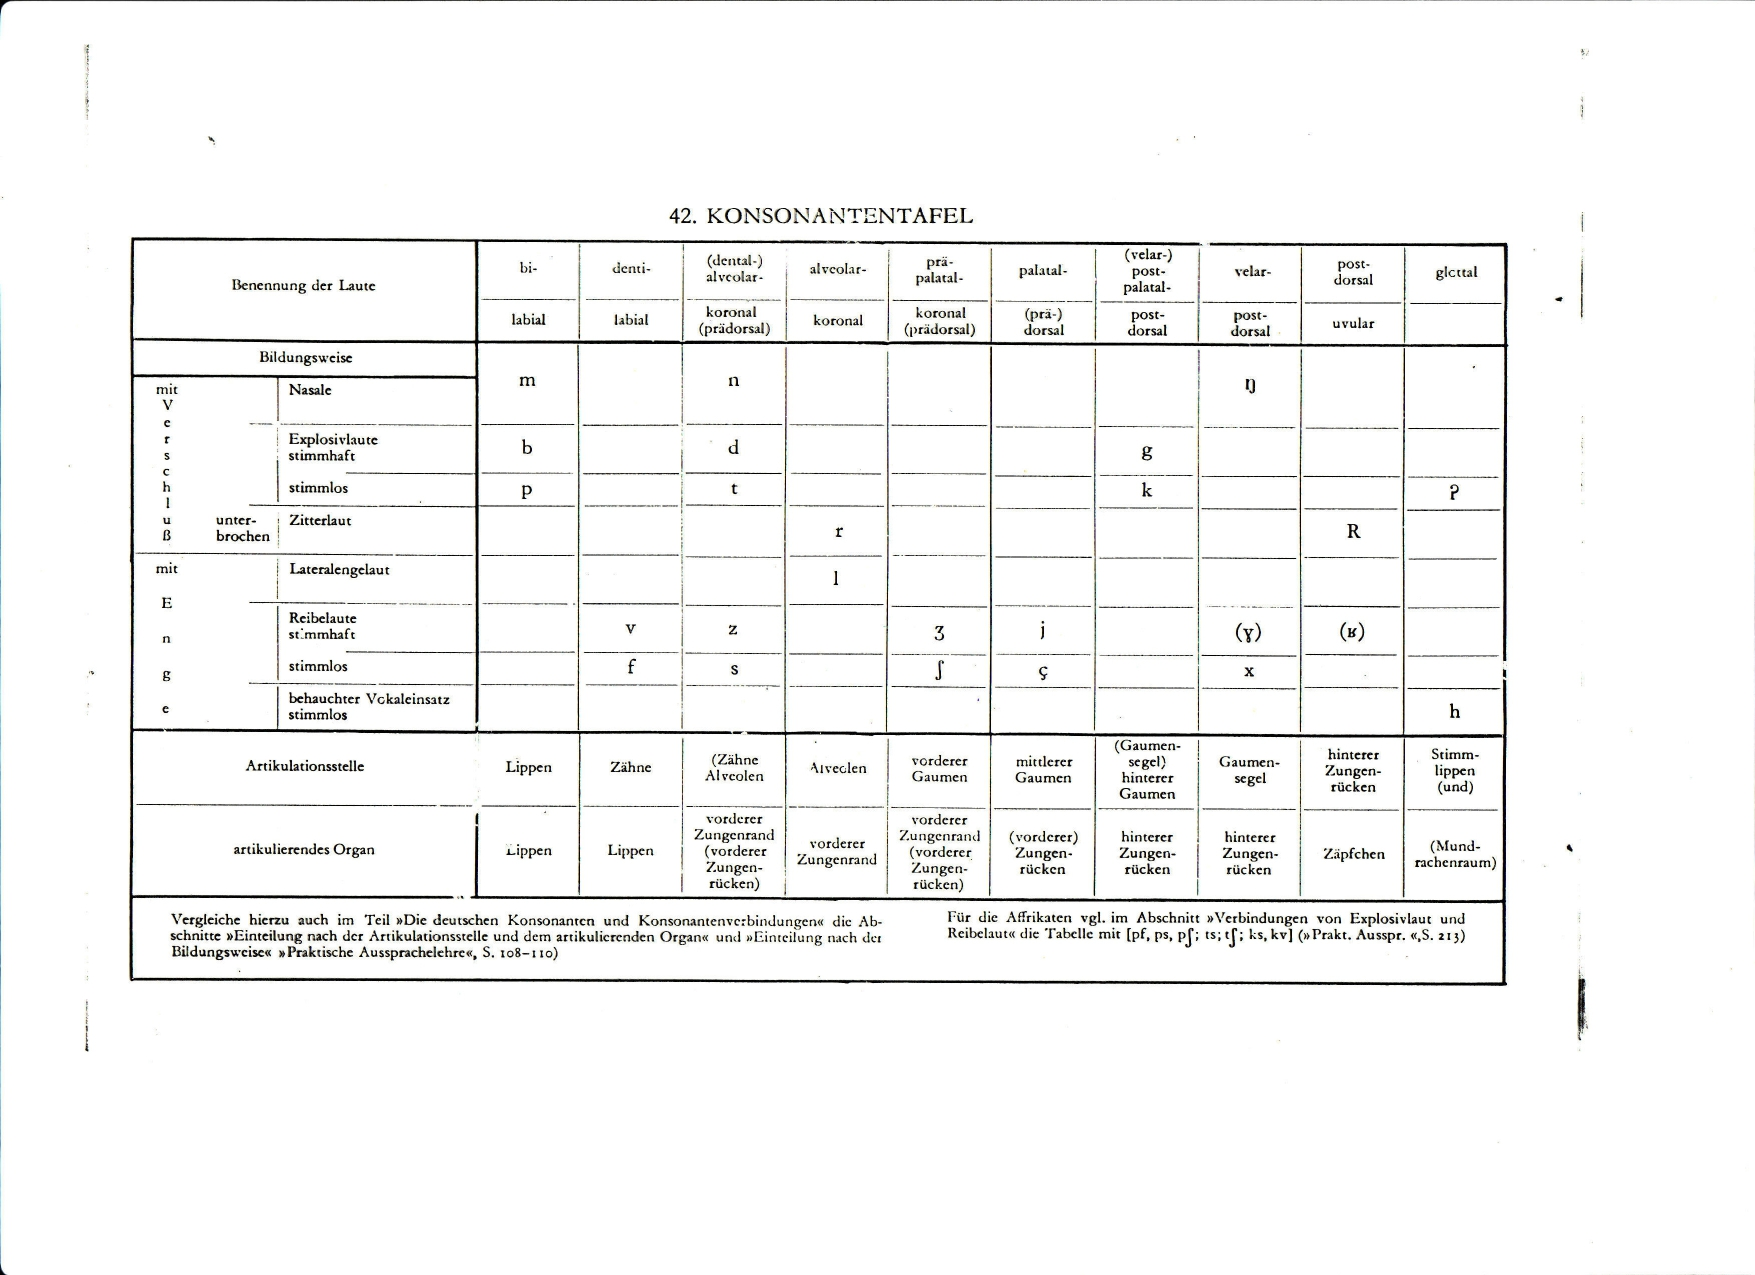
\includegraphics[width=1\textwidth,height=\textheight]{./pictures/02g_Konsonantentafel_page-0001.jpg}

Beschreiben Sie die Bildung des Vokals \ldots{} bzw. des Konsonanten
\ldots{} ! Verwenden Sie Bilder und eventuell vorhandene Animationen!
Führen Sie typische Wortbeispiele an! Zeigen Sie mit den Wortbeispielen
auch, welche Schreibweisen für den betreffenden Sprachlaut möglich sind!

In der Tabelle können Sie erfahren, welche deutschen Sprachlaute Ihnen
zugewiesen wurden.

\hypertarget{aufgabenbereich-der-phonemik}{%
\chapter{Aufgabenbereich der
Phonemik}\label{aufgabenbereich-der-phonemik}}

Die Phonemik erforscht Lautsysteme. Ihre Aufgabe besteht also darin,
``die Beziehungen der Laute einer gegebenen Sprache zueinander zu
analysieren, um so das Lautsystem zu beschreiben.'' (SSM 1: 2) In der
Tagmemik, einer wichtigen Richtung des amerikanischen Strukturalismus
(Hauptvertreter K. L. Pike), werden alle sprachlichen Einheiten unter
drei Gesichtspunkten untersucht:

\begin{itemize}
\item
  Opposition,
\item
  Variation und
\item
  Distribution.
\end{itemize}

\hypertarget{opposition}{%
\subsection{Opposition}\label{opposition}}

Die Wortpaare (oder besser: Lautfolgen) in den folgenden Beispielen
unterscheiden sich jeweils nur durch einen Laut. Diejenigen Laute, die
sich voneinander unterscheiden (also distinktive phonetische Merkmale
aufweisen), stehen in Opposition (nach einer anderen Ausdrucksweise ``in
paradigmatischem Kontrast'') zueinander, womit gesagt sein soll, daß sie
bedeutungsunterscheidende Funktion haben.

\begin{enumerate}
\def\labelenumi{(\arabic{enumi})}
\setcounter{enumi}{7}
\item
  Deutsch: {[}lant{]} ``Land'' vs.~{[}vant{]} ``Wand''\\
  \[
  \frac{[lant]}{[vant]}
  \]
\item
  Slowenisch: {[}ko:s{]} ``kos'' (Stück) vs.~{[}vo:s{]} ``voz''
  (Wagen)\\
  \[
  \frac{[ko:s]}{[vo:s]}
  \]
\item
  Englisch: {[}fɪʃ{]} ``fish'' (Fisch) vs.~{[}dɪʃ{]} ``dish'' (Gefäß).\\
  \[
  \frac{[fɪʃ]}{[dɪʃ]}
  \]
\end{enumerate}

Somit müssen {[}l{]} und {[}v{]} im deutschen Beispiel, {[}k{]} und
{[}v{]} im slowenischen und {[}f{]} und {[}d{]} im englischen jeweils
zwei Phonemen zugeordnet werden: in (8) den Phonemen /l/ und /v/, in (9)
den Phonemen /k/ und /v/ und in (10) den Phonemen /f/ und /d/.

Opposition ist eine \textbf{paradigmatische Beziehung}, Kontrast dagegen
eine syntagmatische. Eine Opposition ist eine \textbf{symmetrische
Beziehung} zwischen sprachlichen Lauten. In den Lautfolgen der Wörter
\textless fast\textgreater{} und \textless Rast\textgreater{} steht der
Obstruent {[}f{]} in Opposition zum Liquid {[}R{]} und umgekehrt.
\textbf{Kontrast} ist dagegen eine \textbf{asymmetrische Beziehung}
zwischen sprachlichen Lauten (vgl. Eisenberg 1998: 88). In einer Form
wie \textless Frau\textgreater{} steht der Liquid /r/ in Kontrast zum
Obstruenten /f/, während der Obstruent /f/ in dieser Position nicht in
Kontrast zum Liquid /r/ stehen kann, da eine (einsilbige) Form wie
{[}rfao{]} nicht vorkommt. In anderen Umgebungen kontrastiert der
Obstruent durchaus mit dem Liquid\emph{,} z.B. in {[}Wurf{]}, aber der
Liquid nicht mit dem Obstruenten {[}Wufr{]}. Beide Lautfolgen (d.h.
{[}fr{]} und {[}rf{]}) sind somit an unterschiedliche Kontexte gebunden.
Der Kontrastbegriff ist die Grundlage für die Ermittlung der
\textbf{phonotaktischen Kombinationsmöglichkeiten} (Lautkombinatorik) in
einer Sprache. Als operationale Verfahren zur Ermittlung einer
\textbf{Opposition} verwenden wir die \textbf{Kommutations- oder
Substitutionsprobe}, zur Ermittlung eines \textbf{Kontrastes} dagegen
die \textbf{Permutations- oder Verschiebeprobe}. Die in den oben
angeführten Beispielen durchgeführte Kommutationsprobe nennt man
übrigens auch den \textbf{Minimalpaartest}. (vgl. auch in der
Dudengrammatik (Drosdowski 1995 : 32-33) über die funktionalen
Eigenschaften Opposition und Kontrast am Beispiel des Wortes
\textless Markt\textgreater).

\hypertarget{variation}{%
\subsection{Variation}\label{variation}}

Zwei verschiedene Laute einer Sprache stehen nicht immer in Opposition
zueinander. Können verschiedene Laute nicht als Phoneme eingeordnet
werden, dann besteht die Möglichkeit, dass es sich um Varianten eines
einzigen Phonems (auch \textbf{Allophone} genannt) handelt.
\textbf{Phonemvariation} kann \textbf{frei} oder
\textbf{stellungsgebunden} sein.

\begin{enumerate}
\def\labelenumi{(\arabic{enumi})}
\setcounter{enumi}{10}
\tightlist
\item
  Deutsch: {[}reː.ɡən{]} vs.~{[}Reː.ɡən{]} vs.~{[}ʁeː.ɡən{]} ``Regen''
\item
  Slowenisch: {[}ta.nək{]} tanek ``dünn'', masc. vs.~{[}taŋ.ka{]} tanka
  ``dünn'', fem.
\end{enumerate}

Im deutschen Wort \textless Regen\textgreater{} (11) kann das Phonem /r/
verschiedentlich realisiert werden, ohne dadurch die Bedeutung der
Lautfolge zu verändern. Im Deutschen sind die drei r-Laute {[}r{]},
{[}R{]} und {[}ʁ{]} freie Varianten eines einzigen Phonems, d.h.
\textbf{fakultative Allophone} des Phonems /r/. Auch im Slowenischen
können die oben genannten r-Laute frei variieren, ohne die Wortbedeutung
zu verändern. In der slowenischen Standardsprache ist allerdings im
Unterschied zur deutschen nur das alveolar apikale {[}r{]} üblich, das
auch als Zungenspitzen-r bekannt ist. In einer anderen Sprache können
verschieden realisierte r-Laute allerdings auch in Opposition zueinander
stehen und somit als zwei verschiedene Phoneme eingeordnet werden (z.B.
im Spanischen ein langer und ein kurzer r-Laut).

Das Phonem /n/ wird im Slowenischen (12) je nach Lautumgebung als
dental-alveolares {[}n{]} oder als velar-postdorsales {[}ŋ{]}
realisiert. Vor einem Vokal wird beispielsweise die erste Variante
ausgesprochen, vor den velaren Obstruenten {[}k{]}, {[}g{]} und {[}x{]}
die letztere (Toporišič \textsuperscript{2}1991: 71). Das Phonem /n/
weist demnach im Slowenischen (neben anderen hier nicht aufgeführten)
zumindest zwei \textbf{stellungsbedingte Allophone} (positionsabhängige,
stellungsgebundene oder kombinatorische Allophone) auf. Im Slowenischen
sind die beiden Allophone \textbf{komplementär verteilt}, d.h. daß das
{[}n{]} nicht in allen Lautumgebungen vorkommt, in denen {[}ŋ{]}
auftritt, und umgekehrt.

Auch im Deutschen kommt der velare Nasalkonsonant {[}ŋ{]} ebenfalls
nicht in allen Lautumgebungen vor (wie im Slowenischen ist er im
Silbenanlaut ausgeschlossen), aber an der Silbengrenze zwischen Vokalen
steht er in Opposition zum alveolaren Nasalkonsonant {[}n{]} (vgl.
\textless Wanne\textgreater{} vs.~\textless Wange\textgreater). Die
Tatsache, dass mit Hilfe eines Minimalpaartests eine Opposition zwischen
den beiden deutschen Nasalkonsonanten gefunden werden konnte, kann man
als Argument für die Unterscheidung zweier Phoneme werten. Dagegen
spricht, dass der velare Nasalkonsonant in weniger Lautumgebungen
vorkommt als der alveolare Nasalkonsonant.

Der phonetische Unterschied in slowenischen Beispiel (12) ist demnach
durch die Lautumgebung bestimmt. Man kann also von der lautlichen
Umgebung her schließen, welchen phonetischen Wert das Phonem /n/ in
dieser Umgebung hat. Somit sind die beiden Laute (Phone) im Slowenischen
Varianten einer Lauteinheit (eines Phonems), und es genügt, ein einziges
phonemisches Zeichen /n/ für beide phonetischen Varianten {[}n{]} und
{[}ŋ{]} anzusetzen. Im Slowenischen wird dieses Verhalten auch in der
Ortographie (Rechtschreibung) ausgedrückt, denn beide
Realisierungsformen des Phonems werden durch das gleiche Graphem
wiedergegeben (auch in Eigennamen, vgl. (13)).

\begin{enumerate}
\def\labelenumi{(\arabic{enumi})}
\setcounter{enumi}{12}
\tightlist
\item
  \textless Ana\textgreater{} vs.~\textless Anka\textgreater.
\end{enumerate}

Im Deutschen spricht die Orthographie nicht dafür, die beiden
Nasalkonsonanten einem einzigen Phonem zuzuordnen, denn die beiden Laute
werden im einheimischen Wortschatz durch unterschiedliche Grapheme
wiedergegeben: so wird der alveolare Nasalkonsonant mit dem Graphem
\textless n\textgreater{} wiedergegeben (wie z.B. in \textless Biene,
Wanne\textgreater), während dem velaren Nasalkonsonanten das Graphem
\textless ng\textgreater{} zugeordnet wird (wie z.B. in \textless Wange,
Klinge, Zunge\textgreater). Die beiden deutschen Nasalkonsonanten
könnten eher als zwei verschiedene Phoneme gewertet werden, die beiden
slowenischen Nasalkonsonanten dagegen eher als ein Phonem (mit
stellungsbedingter Phonemvariation).

\hypertarget{distribution}{%
\subsection{Distribution}\label{distribution}}

Beim Vergleich zweier Sprachen kann man oft feststellen, dass in beiden
zwar derselbe Laut (oder zwei sehr ähnliche Laute) vorkommt, aber
jeweils in unterschiedlicher Position. Der betreffende Laut hat in
beiden Sprachen also eine unterschiedliche Verteilung oder Distribution.
Dieser Umstand soll am Beispiel des velaren Nasalkonsonanten illustriert
werden.

Der \textbf{velare Nasalkonsonant} {[}ŋ{]} kommt in der
\textbf{deutschen Standardsprache} in den folgenden Positionen vor:

\begin{itemize}
\item
  im Wort- und Silbenauslaut nach ungespannten Vokalen (z.B.
  \textless Ding, eng, Gang, Gong, Dung\textgreater);
\item
  im Wort- und Silbenauslaut als Folge der Schwa-Tilgung und der
  Assimilation nach {[}g{]} und {[}k{]} in derselben Silbe (z.B.
  \textless fragen, packen\textgreater);
\item
  im Silbenauslaut vor {[}k{]} im Anlaut der nächsten Silbe (z.B.
  \textless trin-ken\textgreater);
\item
  im Silbenauslaut vor {[}g{]} im Anlaut der nächsten Silbe, aber nur in
  Lehnwörtern (z.B. \textless Tan-go, Un-garn, Lin-gu-ist\textgreater);
\item
  im Wort- und Silbeninlaut vor {[}k{]} in derselben Silbe (z.B.
  \textless Schank\textgreater);
\item
  im Inlaut als sogenanntes Silbengelenk (d.h. gleichzeitig im Auslaut
  der ersten Silbe und im Anlaut der zweiten) vor Schwa {[}ə{]} (z.B.
  \textless hängen\textgreater) oder als Folge von Assimilation vor
  sonantischem {[}l̩{]} (z.B. kling(e)ln).
\end{itemize}

In der \textbf{slowenischen Standardsprache} tritt der \textbf{velare
Nasalkonsonant} {[}ŋ{]} in den folgenden Positionen auf:

\begin{itemize}
\item
  im Silbenauslaut nach ungespannten Vokalen vor {[}g{]}, {[}k{]} und
  {[}x{]} in der nächsten Silbe (z.B. \textless An-hovo, Kon-go,
  Can-kar\textgreater);
\item
  im Silbeninlaut nach ungespannten Vokalen vor {[}k{]} in derselben
  Silbe (z.B. \textless tank\textgreater).
\end{itemize}

Aus dieser Gegenüberstellung ist ersichtlich, daß die
\textbf{Distribution} des velaren Nasalkonsonanten \textbf{im
Slowenischen eingeschränkter} ist als im Deutschen, denn im Slowenischen
kann er nicht stehen:

\begin{itemize}
\item
  im Silben- oder Wortauslaut, wenn kein {[}k{]} in derselben oder der
  nächsten Silbe folgt;
\item
  im Inlaut vor Schwa {[}ə{]} oder sonantischem {[}l̩{]};
\item
  im Auslaut nach {[}g{]} und {[}k{]} (d.h. aufgrund von Schwa-Reduktion
  und regressiver Nasalassimilation an einen velaren Obstruenten wie im
  deutschen Verb \textless fragen\textgreater).
\end{itemize}

\textbf{Tabelle 2: Distribution des Nasalkonsonaten {[}ŋ{]} im Deutschen
und Slowenischen}

\begin{longtable}[]{@{}
  >{\raggedright\arraybackslash}p{(\columnwidth - 4\tabcolsep) * \real{0.2857}}
  >{\raggedright\arraybackslash}p{(\columnwidth - 4\tabcolsep) * \real{0.5000}}
  >{\raggedright\arraybackslash}p{(\columnwidth - 4\tabcolsep) * \real{0.2063}}@{}}
\toprule()
\begin{minipage}[b]{\linewidth}\raggedright
\end{minipage} & \begin{minipage}[b]{\linewidth}\raggedright
\textbf{Deutsch}
\end{minipage} & \begin{minipage}[b]{\linewidth}\raggedright
\textbf{Slowenisch}
\end{minipage} \\
\midrule()
\endhead
\textbf{Wort- u.} \textbf{Silbenanlaut} & & \\
\textbf{Wort- u.} \textbf{Silbeninlaut} & vor {[}k{]} & vor {[}k{]} \\
\textbf{Wortinlaut} \textbf{(Silbengelenk)} & vor {[}ə{]} und {[}l̩{]}
& \\
\textbf{Silbenauslaut} & Vokal:

vor {[}k{]} & Vokal:

vor {[}k{]}, {[}g{]}, {[}x{]} \\
\textbf{Wortauslaut} & nach {[}g{]} und {[}k{]} in unbetonter Silbe (bei
Schwa-Tilgung) & \\
\bottomrule()
\end{longtable}

~

In einem Fall ist die Distribution des velaren Nasalkonsonanten im
Deutschen jedoch eingeschränkter, denn im Slowenischen kann der velare
Nasalkonsonant vor {[}x{]} in der nächsten Silbe auftreten, im Deutschen
jedoch nicht.

Beide Sprachen haben u.a. gemeinsam, daß der velare Nasalkonsonant nicht
im Silbenanlaut vorkommen kann. Diese Möglichkeit besteht in anderen
Sprachen, z.B. im Kulunge, einer Sprache Nepals (SSM 1: 3).

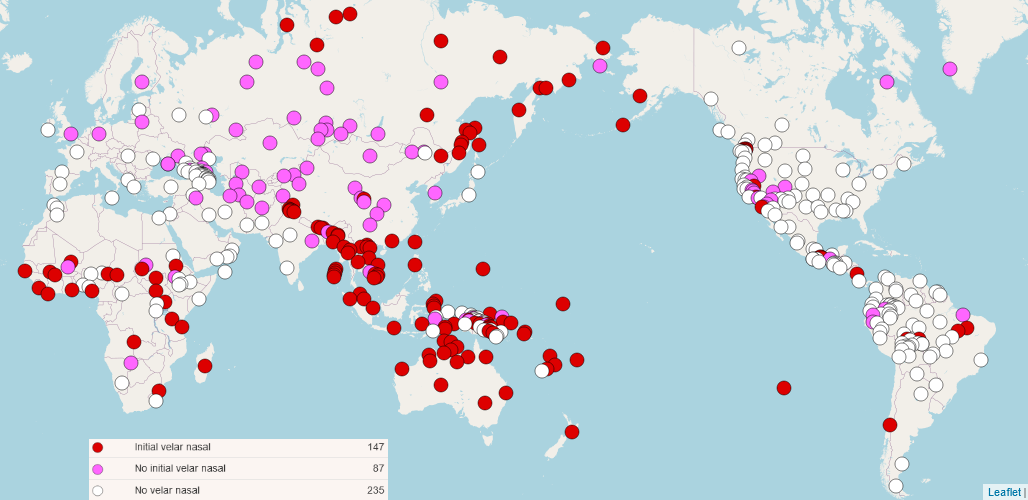
\includegraphics[width=1\textwidth,height=\textheight]{./pictures/01b_NSG_Intro_2020-10-07/wals_velar_nasal.png}

\href{https://wals.info/}{Wals Online}

Im Rahmen der Lautdistribution wird auch die Häufigkeit des Vorkommens
eines Lautes untersucht, anhand derer sich oft charakteristische
Unterschiede zwischen Sprachen feststellen lassen (SSM 1: 3). So tritt
z.B. der stimmhafte postalveolare Frikativ {[}ʒ{]} im Deutschen nur in
wenigen Lehnwörtern auf (z.B. \textless{}\uline{G}enie,
Gara\uline{g}e\textgreater) und hat daher eine eher periphere Stellung
im deutschen Phonemsystem. Im Französischen oder im Slowenischen tritt
dieser stimmhafte Frikativ jedoch in einer viel größeren Anzahl von
Wörtern auf und gehört eher zum Kern des französischen bzw. slowenischen
Phonemsystems (z.B. franz. \textless{}\uline{j}e\textgreater{} ``ich'',
\textless{}\uline{j}our\textgreater{} ``Tag'',
\textless pi\uline{g}eon\textgreater{} ``Taube''; slow.
\textless{}\uline{ž}ena\textgreater{} ``(Ehe)frau'',
\textless{}\uline{ž}oga\textgreater{} ``Ball'',
\textless{}\uline{ž}aba\textgreater{} ``Frosch'').

\hypertarget{phonem--und-silbeninventare}{%
\subsection{Phonem- und
Silbeninventare}\label{phonem--und-silbeninventare}}

Zur Orientierung sollen einige Angaben zur Phoneminventargröße
herangezogen werden. In der Untersuchung von Ian Maddieson (Consonant
Inventories, In: Wals 2005) findet man folgende Angaben zur
\textbf{Größe von Konsonanteninventaren} in den Sprachen der Welt
(gemeint sind Konsonantenphoneme):

\begin{longtable}[]{@{}ccc@{}}
\toprule()
~ & \textbf{Consonant Inventory Size} & ~ \\
\midrule()
\endhead
1. & Small & 91 \\
2. & Moderately small & 121 \\
3. & Average & 181 \\
4. & Moderately large & 116 \\
5. & Large & 53 \\
@ & Total & 562 \\
\bottomrule()
\end{longtable}

~

\begin{itemize}
\item
  Die \textbf{typischere Konsonanteninventargröße} liegt in den unteren
  Zwanzigern, wobei der Mittelwert für die 562 Sprachen 22,7 beträgt,
  der Modus 22 und der Median 21. Konsonanteninventare in der Nähe
  dieser Größe (\textbf{22 ± 3}) wurden als \textbf{durchschnittlich}
  kategorisiert, und der Rest unterteilt in die Kategorien klein (von 6
  bis 14 Konsonanten), mäßig klein (15-18), mäßig groß (26-33) und groß
  (34 oder mehr Konsonanten).
\item
  \textbf{Slowenisch} kann wie \textbf{Deutsch} oder Britisches Englisch
  in die Gruppe mit \textbf{durchschnittlich} vielen Konsonantenphonemen
  (»average«) eingeordnet werden (19~ Konsantenphoneme: p, t, k, b, d,
  g, f, v, s, z, s, S, j, Z, x, m, n, r, l).
\item
  Rotokas (West Bougainville; Papua-Neuguinea) hat nur sechs
  Konsonanten: /p, t, k, b, d, g/. !Xóõ (Southern Khoisan; Botswana) hat
  122 Konsonanten, hauptsächlich weil es sehr viele verschiedene
  Klicklaute gibt, mit denen ein Wort beginnen kann.
\end{itemize}

~

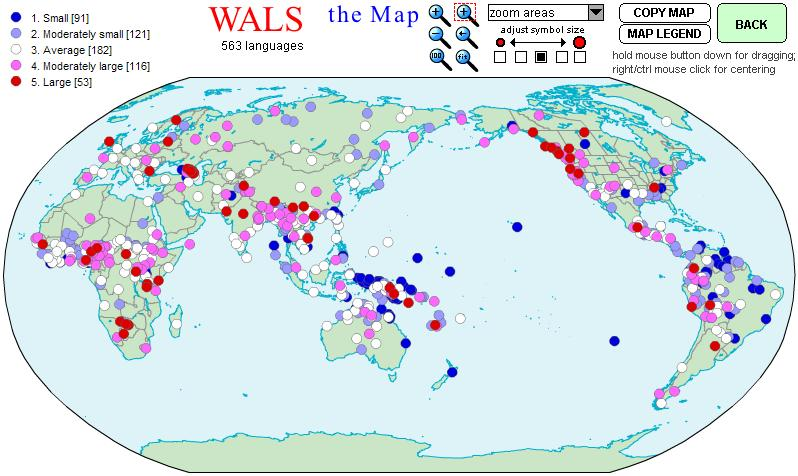
\includegraphics[width=1\textwidth,height=\textheight]{./pictures/01b_NSG_Intro_2020-10-07/wals_consonant_inventories.png}

\href{https://wals.info/}{Wals Online}

In Maddieson (in: Wals 2005) finden wir folgende Angaben zur Größe von
\textbf{Vokalinventaren} (gemeint sind Vokalphoneme):

\begin{longtable}[]{@{}cccc@{}}
\toprule()
~ & \textbf{Vowel Quality Inventory} & ~ & ~ \\
\midrule()
\endhead
1. & Small vowel inventory & (2-4) & 92 \\
2. & Average vowel inventory & (5-6) & 288 \\
3. & Large vowel inventory & (7-14) & 183 \\
§ & Total & ~ & 563 \\
\bottomrule()
\end{longtable}

\href{https://wals.info/}{Wals Online}

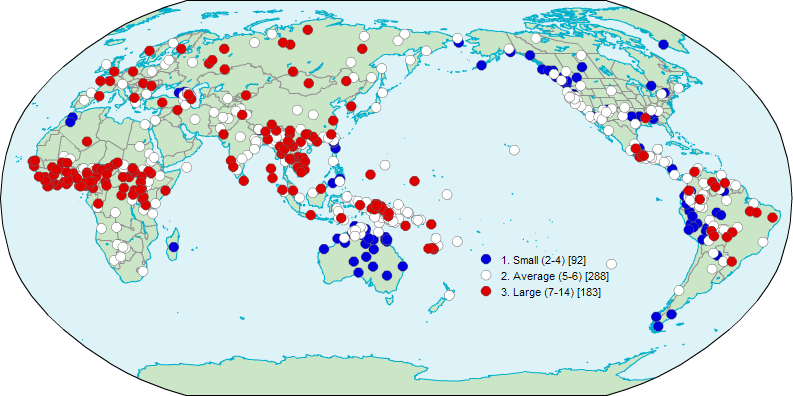
\includegraphics[width=1\textwidth,height=\textheight]{./pictures/01b_NSG_Intro_2020-10-07/wals_vowel_inventories.png}

~

\begin{itemize}
\item
  Der \textbf{Umfang} des kleinsten erfassten Vokalqualitätsinventars
  ist 2 und des größten 14.
\item
  Es gibt 4 Sprachen in der Stichprobe mit \textbf{nur zwei}
  kontrastierenden Vokalqualitäten. Ein Beispiel für dieses Extrem ist
  Yimas (Lower Sepik-Ramu; Papua-Neuguinea).«
\item
  Nur eine Sprache in der Stichprobe, \textbf{Deutsch}, verwendet 14
  Vokalqualitäten (i, I, e, E, a, A, O, o, U, u; y, Y, 9, 2; die
  Phonemvarianten @ in \emph{bitt\uline{e}} und 6 in
  \emph{bess\uline{er} nicht berücksichtigt}) »und nur 2 verwenden 13
  Vokalqualitäten, nämlich die hier enthaltene Variante des britischen
  Englisch and Bété (Kru, Niger-Congo; Côte d'Ivoire).
\item
  Deutlich mehr Sprachen haben einen Bestand von \textbf{fünf Vokalen}
  als jede andere Zahl -- 188 oder etwas mehr als ein Drittel. Die
  zweithäufigste Inventargröße sind \textbf{sechs Vokalqualitäten} mit
  100 Sprachen (oder 17,8\% der Stichprobe).
\item
  Vokalqualitätsinventare mit 5 oder 6 Mitgliedern wurden in der
  Kategorie „Durchschnitt'' zusammengefasst, während solche mit 4 oder
  weniger als „klein'' und solche mit 7 oder mehr als „groß'' eingestuft
  werden. Sprachen mit „durchschnittlicher'' Vokalinventargröße machen
  mehr als die Hälfte der Stichprobe aus (51,2 \%), etwa ein Drittel
  (32,5\%) hat „große'' Vokalqualitätsinventare und nur 16,3 \% haben
  „kleine'' Vokalqualitätsinventare.
\item
  \textbf{Slowenisch} verfügt in betonten Silben über 7 verschiedene
  Vokalqualitäten, die distinktiv genutzt werden (i, e, E, a, O, o, u)
  und kann damit (mit nur etwa halb so vielen distinktiv genutzten
  Vokalqualitäten) in dieselbe Gruppe eingeordnet werden wie
  \textbf{Deutsch} oder \textbf{Britisches Englisch}, die (mit 14 bzw.
  13 distinktiv genutzten Vokalqualitäten) am oberen Ende dieser Gruppe
  anzusiedeln sind.
\item
  \textbf{In unbetonten Silben} ist die Anzahl der distinktiv genutzten
  Vokalqualitäten gewöhnlich kleiner, so auch im \textbf{Slowenischen}
  (keine hohen oder mittelhohen Vokale i, e, u) und \textbf{Deutschen}
  (lediglich @, 6).
\end{itemize}

\textbf{Konsonanten-Vokal-Verhältnis} in den Sprachen der Welt
(Maddieson, in Wals 2005):

\begin{itemize}
\item
  Das Verhältnis wird einfach durch Division der Anzahl der Konsonanten
  (C) durch die Anzahl der Vokalqualitäten (VQ) berechnet und wird als
  C/VQ-Verhältnis bezeichnet.
\item
  Die resultierenden Zahlen reichen von einem Tief von nur etwas über 1
  bis zu einem Hoch von 29. Der niedrigste Wert unter den 563 Sprachen,
  für die er berechnet wurde, wird von Andoke (isoliert; Kolumbien)
  repräsentiert, das 10 Konsonanten und 9 Vokalqualitäten hat. Die
  höchste Zahl wird von Abkhaz (Nordwestkaukasier; Georgien)
  repräsentiert, das mit 58 Konsonanten, aber nur 2 Vokalqualitäten
  analysiert wird. Das Verhältnis bewegt sich somit zwischen 1,11 und
  29, aber die häufigeren Werte liegen näher am unteren Ende der Spanne:
  der Mittelwert beträgt 4,25 und der Median 3,5.
\item
  Die Sprachen wurden in fünf Kategorien eingeteilt, basierend auf der
  Aufteilung des Bereichs in geeignete Schritte unterhalb, nahe und
  oberhalb des Medians, um ein Histogramm mit annähernd normaler
  Verteilung zu erstellen. Sprachen mit einem Verhältnis von 2,0 oder
  weniger wurden als „niedriges'' C/VQ-Verhältnis eingestuft. Diejenigen
  mit einem Verhältnis über 2,0, aber unter 2,75 wurden als „mäßig
  niedrig'' eingestuft. Personen mit einem Verhältnis von 2,75 oder
  höher aber kleiner als 4,5 wurden als „durchschnittlich'', solche mit
  Werten von 4,5 oder höher aber kleiner als 6,5 als „mäßig hoch'' und
  solche mit Werten über 6,5 als „hoch'' eingestuft. Nur 10 Sprachen
  haben Verhältnisse von 12 oder höher.«
\item
  \textbf{Slowenisch} gehört in die Gruppe »\textbf{moderately low}«,
  \textbf{Deutsch} und \textbf{Britisches Englisch} aufgrund der vielen
  distinktiv genutzten Vokalqualitäten in die Gruppe »\textbf{low}«. ~
\end{itemize}

~

\begin{longtable}[]{@{}ccc@{}}
\toprule()
~ & \textbf{Consonant-Vowel-Ratio} & ~ \\
\midrule()
\endhead
1. & Low & 59 \\
2. & Moderately low & 97 \\
3. & Average & 234 \\
4. & Moderately high & 102 \\
5. & High & 71 \\
total & 563 & ~ \\
\bottomrule()
\end{longtable}

\href{https://wals.info/}{Wals Online}

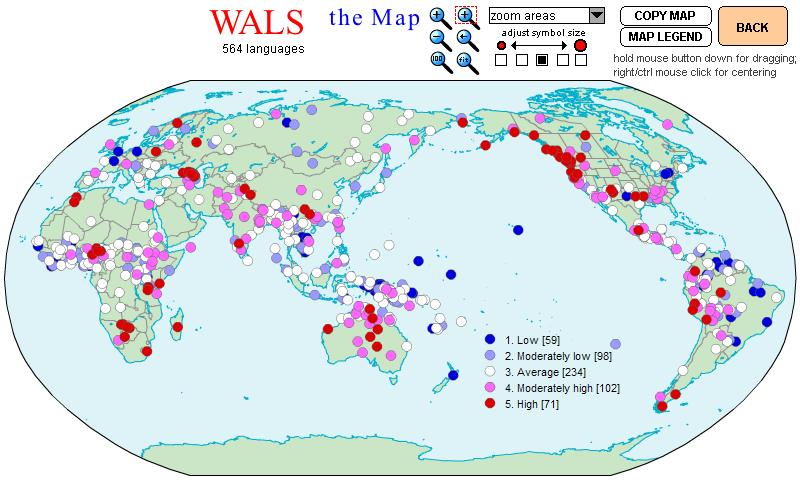
\includegraphics[width=1\textwidth,height=\textheight]{./pictures/01b_NSG_Intro_2020-10-07/wals_vowel_consonant_ratio.png}

\hypertarget{sec-artikulation}{%
\chapter{Artikulatorische Phonetik}\label{sec-artikulation}}

Im Fremdsprachenunterricht schenken wir der artikulatorischen Phonetik
gewöhnlich große Aufmerksamkeit.

Die \textbf{Artikulation} bezieht sich auf intentional gesteuerte
Bewegungen der Sprechwerkzeuge zur Bildung von Sprachlauten. (Bußmann
1990 : 99)

Im Rahmen der artikulatorischen Phonetik beschreiben wir also, wie die
deutschen Sprachlaute im Einzelnen gebildet werden. Dazu benötigen wir
einige grundlegende Kenntnisse anderer Wissenschaften, und zwar
insbesondere der \emph{Anatomie} und der \emph{Physik}.

\hypertarget{sec-phonotaktik}{%
\chapter{Phonotaktik}\label{sec-phonotaktik}}

\hypertarget{silbentypen-in-den-sprachen-der-welt}{%
\section{Silbentypen in den Sprachen der
Welt}\label{silbentypen-in-den-sprachen-der-welt}}

Silbentypen in den Sprachen der Welt (Maddieson, in: Wals 2005).

\begin{itemize}
\item
  Die einzige Silbenart, die \textbf{in jeder Sprache} vorzukommen
  scheint, ist \textbf{CV}, dh eine Silbe, die aus nur einem Konsonanten
  vor einem Vokal besteht. In relativ wenigen Sprachen ist dies die
  einzige erlaubte Silbenart. Zu diesen Sprachen gehören Hawaiianisch
  und Mba (Adamawa-Ubangian, Niger-Kongo; Demokratische Republik Kongo).
  Häufiger findet man Sprachen, in denen der Anfangskonsonant nicht
  erlaubt ist, wie zum Beispiel in Fidschian, Igbo (Niger-Kongo;
  Nigeria) und Yareba (Yareban; Papua-Neuguinea). Für diese Sprachen
  kann die kanonische Silbe als (C)V dargestellt werden, wobei die
  Klammern angeben, dass ein Anfangskonsonant ein optionales Element
  ist. Wenn eine Sprache nur Silben zulässt, die in diese Vorlage
  passen, spricht man von einer einfachen Silbenstruktur.
\item
  Eine etwas \textbf{aufwändigere Silbenstruktur} verfügt über einen
  weiteren Konsonanten, entweder am Ende der Silbe oder am Anfang, was
  die Strukturen CVC und CCV ergibt; beides sind mäßige Erweiterungen
  des einfachen CV-Silbentyps. Es lohnt sich jedoch, zwischen zwei Arten
  von zweigliedrigen Konsonantenketten zu unterscheiden. In einer sehr
  großen Anzahl von Sprachen sind zwar zwei Konsonanten am Anfang einer
  Silbe erlaubt, es gibt jedoch strenge Grenzen für die zulässigen
  Kombinationen. Der zweite von zwei Konsonanten ist gewöhnlich darauf
  beschränkt, einer aus einer kleinen Menge zu sein, die entweder zur
  Klasse der Liquide oder der Klasse der Gleitlaute gehört. Die Liquide
  sind die Laute, die üblicherweise durch die Buchstaben
  \textless r\textgreater{} und \textless l\textgreater{} dargestellt
  werden, während Glides vokalähnliche Konsonanten sind, wie die am
  Anfang der slowenischen Wörter \textless vlak\textgreater{} und
  \textless jarem\textgreater. Liquiden und Gleitlauten ist gemeinsam,
  dass ihre Bildung einen relativ ungehinderten Luftstrom aus dem Mund
  ermöglicht. Sprachen, die einen einzelnen Konsonanten nach dem Vokal
  zulassen und/oder zwei Konsonanten vor dem Vokal zulassen, sich aber
  nur an die oben beschriebenen üblichen zweigliedrigen
  Konsonantenmuster halten, werden als \textbf{mäßig komplexe
  Silbenstruktur} gezählt. Ein Beispiel ist Darai (Indoarisch; Nepal).
  Hier ist CCVC die am stärksten erlaubte Silbe, wie in /bwak/ „(sein)
  Vater'', aber der einzig mögliche zweite Konsonant in einer Folge von
  zwei ist /w/.
\item
  Sprachen, die freiere Kombinationen von zwei Konsonanten in der
  Position vor einem Vokal oder drei oder mehr Konsonanten in dieser
  Anfangsposition und/oder zwei oder mehr Konsonanten in der Position
  nach dem Vokal zulassen, werden als \textbf{komplexe Silbenstruktur}
  klassifiziert. Ein offensichtliches Beispiel für eine komplexe
  Struktur ist das Englische, dessen kanonisches Silbenmuster oft als
  (C)(C)(C)V(C)(C)(C)(C) zitiert wird. Die volle Ausdehnung des Musters
  findet nur in wenigen Wörtern statt, wie zum Beispiel
  \textless strengths\textgreater, wenn sie /strENkTs/ ausgesprochen
  werden, aber es ist relativ einfach, Silben zu finden, die mit drei
  Konsonanten beginnen oder mit vier enden, wie in
  \textless split\textgreater{} und \textless texts\textgreater{}
  (/tEksts/).
\item
  Die Einteilung von Sprachen in drei Kategorien der Silbenkomplexität
  (einfach, moderat und komplex) übersieht natürlich viele andere Fragen
  der Segmentverteilung (zum Beispiel, ob die Silben am Anfang und am
  Ende von Wörtern die gleichen oder andere Einschränkungen haben als
  die wortinternen) oder wichtige Unterschiede außer Acht lassen, wie
  selten oder häufig die komplexeren Silbentypen in einer bestimmten
  Sprache vorkommen. Wenn zum Beispiel einige Arten von
  Konsonantensequenzen erst kürzlich durch das Entlehnen internationaler
  Wörter (wie Sport oder Golf) in eine Sprache eingeführt wurden, wird
  die Sprache nach dem, was im etablierteren Vokabular vorkommt,
  klassifiziert. Trotz ihres zusammenfassenden Charakters bietet die
  Drei-Wege-Klassifikation eine sinnvolle Gruppierung mit interessanten
  geografischen Merkmalen.
\item
  \textbf{Slowenisch} und \textbf{Deutsch} lassen sich wie Englisch in
  die Gruppe der Sprachen mit \textbf{komplexen Silbenstrukturen}
  einordnen.
\end{itemize}

\begin{longtable}[]{@{}ccc@{}}
\toprule()
~ & \textbf{Complexity of Syllable structure} & ~ \\
\midrule()
\endhead
1. & Simple syllable structure & 61 \\
2. & Moderately complex syllable structure & 274 \\
3. & Complex syllable structure & 150 \\
@ & total & 485 \\
\bottomrule()
\end{longtable}

\href{https://wals.info/}{Wals Online}

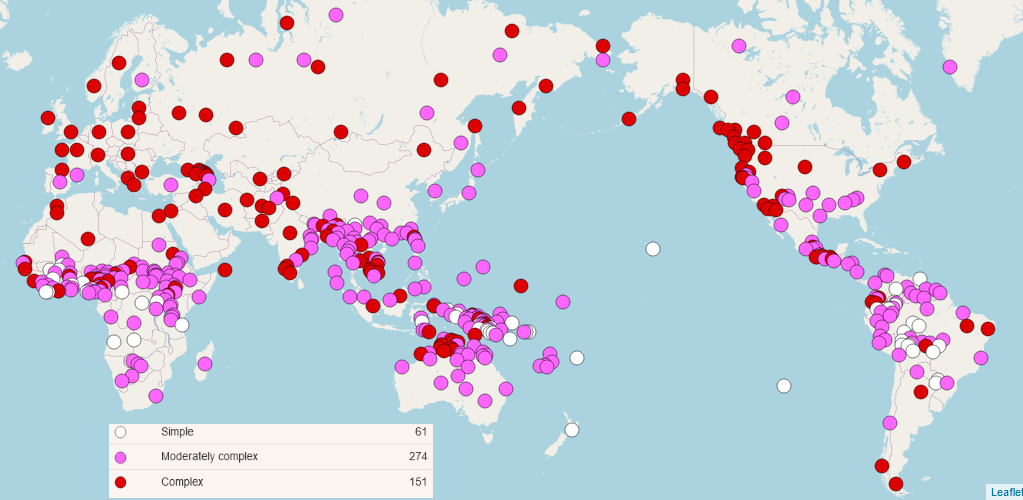
\includegraphics[width=1\textwidth,height=\textheight]{./pictures/01b_NSG_Intro_2020-10-07/wals_syllable_structure.png}

\begin{center}\rule{0.5\linewidth}{0.5pt}\end{center}

\hypertarget{sonorituxe4tshierarchie}{%
\section{Sonoritätshierarchie}\label{sonorituxe4tshierarchie}}

Zusammenstellung, beruhend auf Lewhrwerken bzw. Präsentationen von Utz
Maas, Karl-Heinz Wagner und der Dudengrammtik.

Die Silbe im Vergleich zum Morphem:

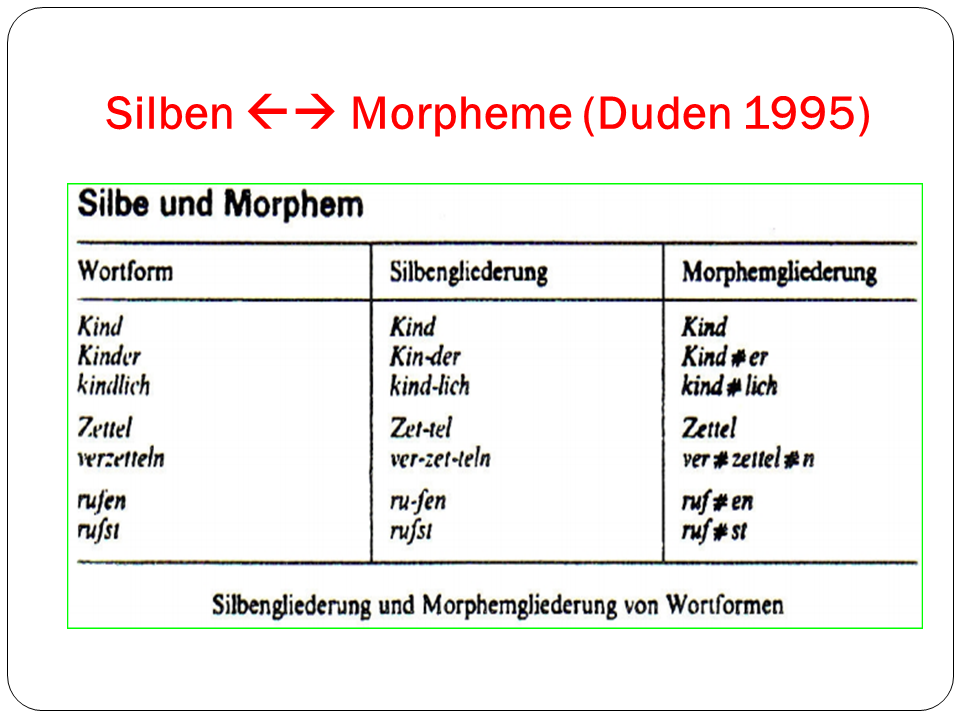
\includegraphics[width=1\textwidth,height=\textheight]{./pictures/Wagner_Maas_Duden_Petric_2.PNG}

Das \textbf{Morphem} ist ein sprachliche Einheit, die wir mit einer
invarianten Bedeutung assoziieren können. Deshalb kann man das Morphem
als bedeutungstragende sprachliche Einheit definieren.

Im Gegensatz zum Morphem können wir \textbf{Phonemen} keine invariante
Bedeutung zuordnen (abgesehen von ikonischen Bedeutungsanteilen - z.B.
die Namen für einen großen und einen kleinen Fisch stimmen nicht selten
überein mit der Größe des Vokalraums bei der Artikulation eines engen
Vokals wie /i/ und eines offenen Vokals wie /a/). Phoneme sind jedoch in
einer Sprache in der Lage, Bedeutungen zu \emph{unterscheiden}. Deshalb
kann man das Phonem als bedeutungsunterscheidende sprachliche Einheit
ansehen.

Eine \textbf{Silbe} kann man als Laut- oder Phonemfolge beschreiben. So
wie Phoneme und Laute keine invariante Bedeutung aufweisen, ist das auch
bei Silben der Fall.

Die \emph{Aufeinanderfolge der Phoneme} in einer Silbe ist nicht
beliebig. In jeder Sprache gibt es eine begrenzte Anzahl von
Kombinationsmöglichkeiten unter den theoretisch möglichen. Ein bekannter
Ansatz zur Erklärung, welche Reihenfolgen von Phonemen in Silben zu
erwarten sind, ist die \textbf{Sonoritätshierarchie}.

Die \textbf{Silbe} kann demnach als Phonemfolge definiert werden, die
auf der Sonoritätshierarchie der Lautklassen beruht.

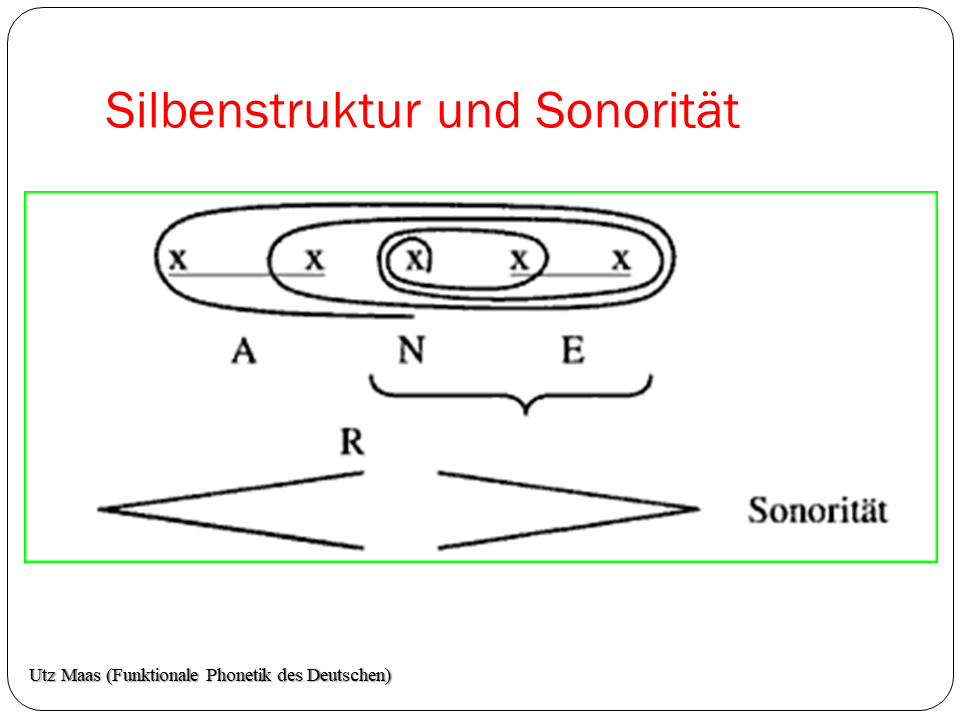
\includegraphics[width=1\textwidth,height=\textheight]{./pictures/Wagner_Maas_Duden_Petric_3.PNG}

Ausgangspunkt für die Anwendung der Sonoritätshierarchie auf die
Beschreibung der Silbenstruktur ist die Beobachtung, dass man bestimmte
Laute bzw. Lautklassen besser \textbf{wahrnehmen} kann als andere. Wie
gut ein Laut wahrnehmbar ist, hängt von verschiedenen
\textbf{Gesichtspunkten} ab: z.B. bei der Artikulation des Vokals /a/
ist das Ansatzrohr (``der Mund'') sehr offen, ganz im Gegensatz zu einem
Konsonanten wie /p/. Außerdem dauert ein Vokal wie /a/ länger als ein
/p/. Auch der Stimmton hilft, den Vokal besser wahrzunehmen. In der
Phonologie werden oft noch weitere Kriterien verwendet, um die Sonorität
(d.h. die Wahrnehmbarkeit) der Lautklassen zu unterscheiden und zu
rangieren. Die Anwendung der verschiedenen möglichen phonetischen
Kriterien führt zur Bildung von \textbf{Sonoritätsskalen}.

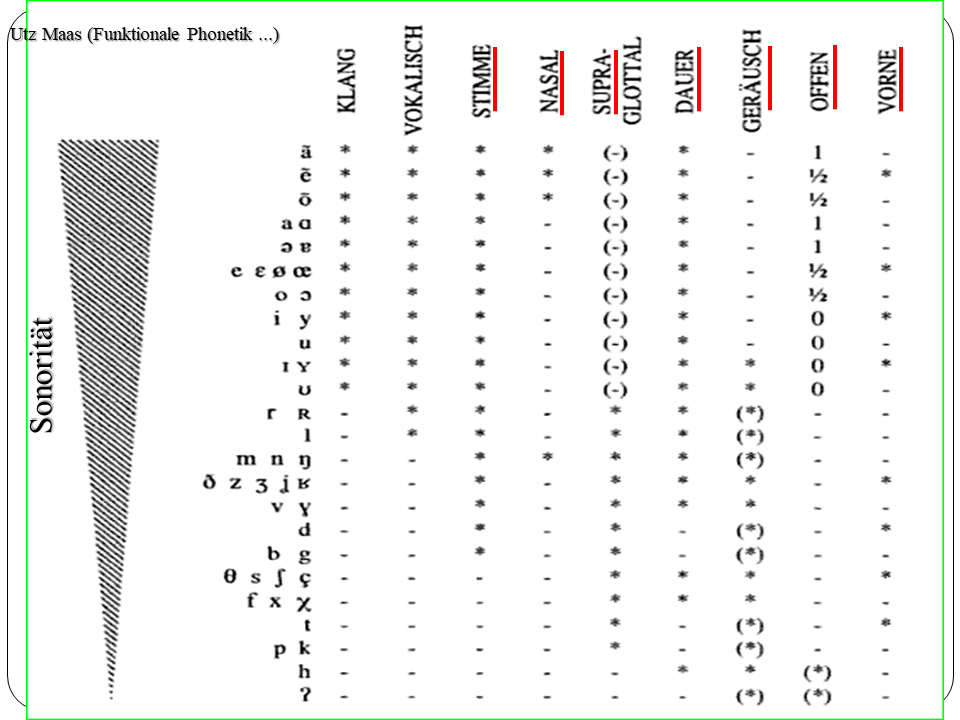
\includegraphics[width=1\textwidth,height=\textheight]{./pictures/Wagner_Maas_Duden_Petric_4.PNG}

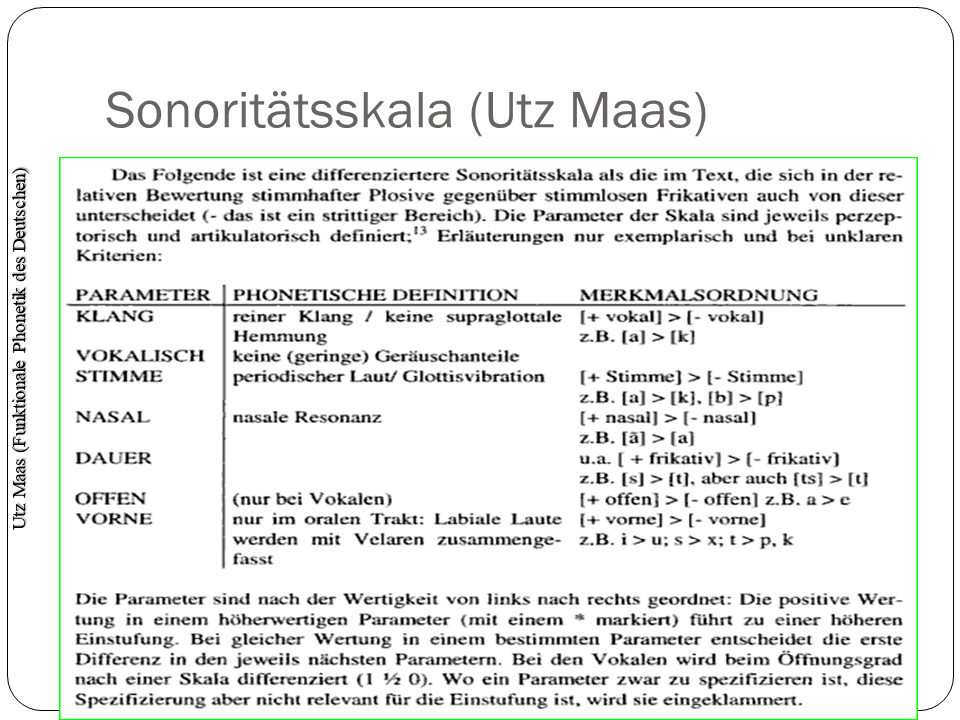
\includegraphics[width=1\textwidth,height=\textheight]{./pictures/Wagner_Maas_Duden_Petric_5.PNG}

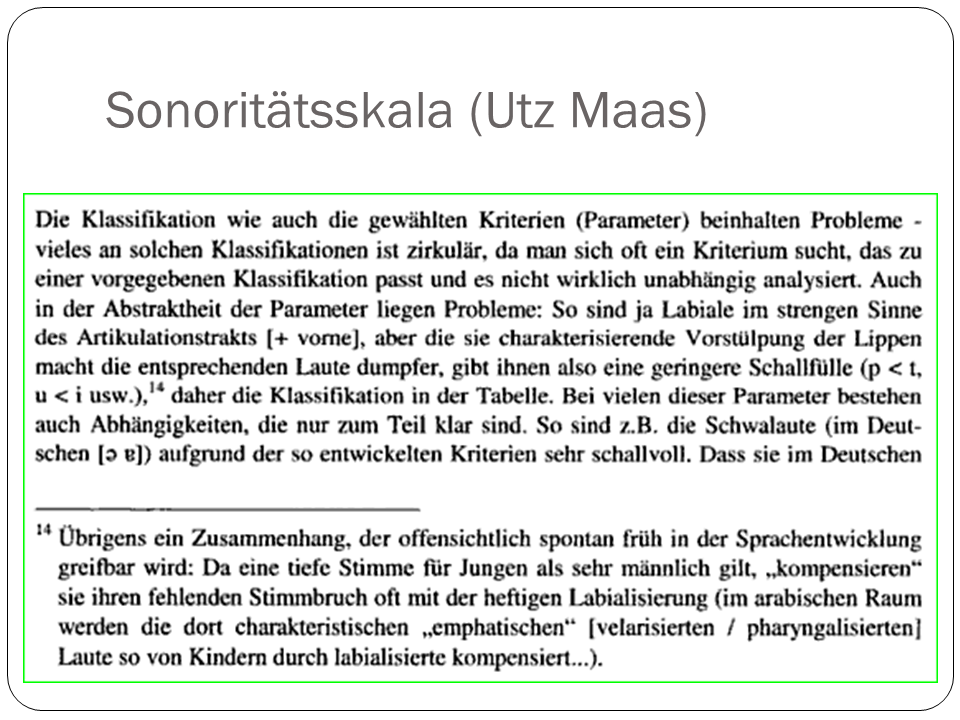
\includegraphics[width=1\textwidth,height=\textheight]{./pictures/Wagner_Maas_Duden_Petric_6.PNG}

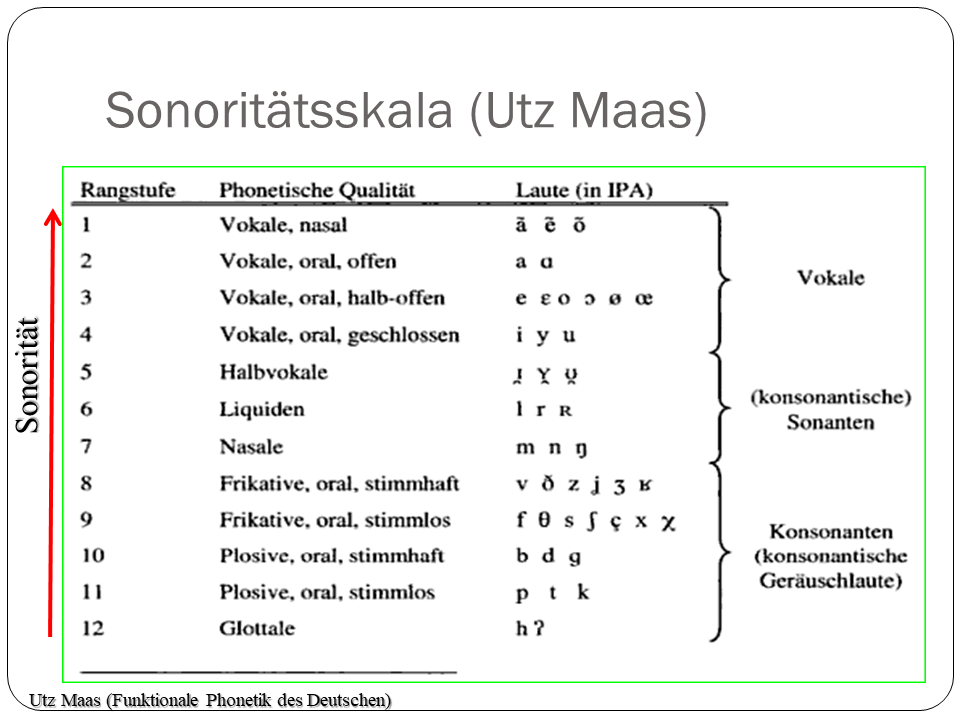
\includegraphics[width=1\textwidth,height=\textheight]{./pictures/Wagner_Maas_Duden_Petric_7.PNG}

Die Sonorität einer Silbe nimmt vom Anlaut zum Silbenkern (gewöhnlich
einem Vokal) zu, nach dem Silbenkern nimmt die Sonorität wieder ab.

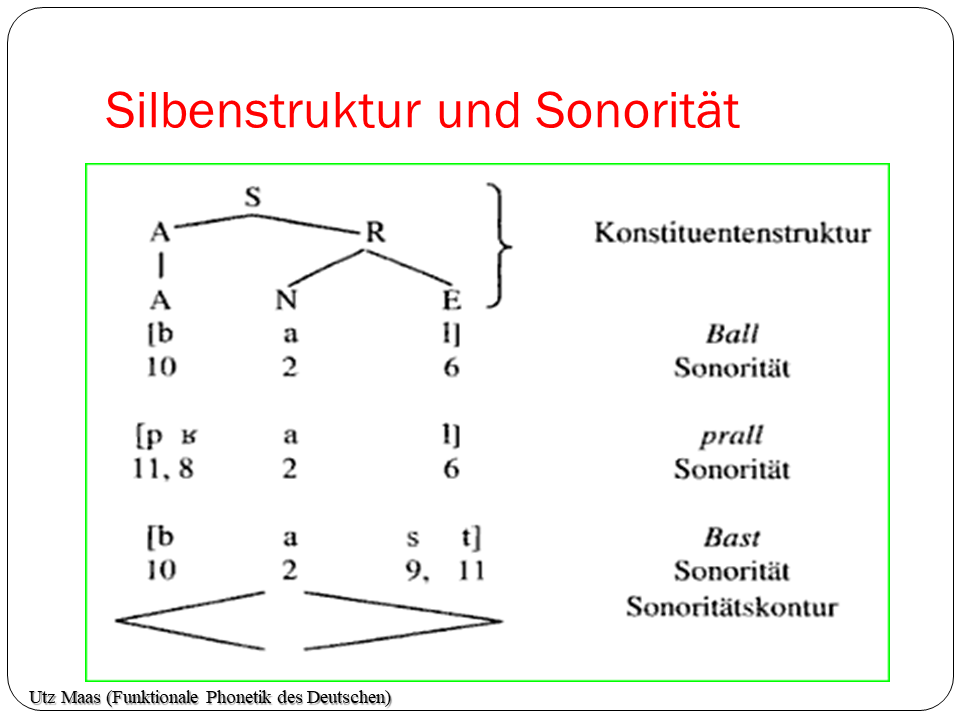
\includegraphics[width=1\textwidth,height=\textheight]{./pictures/Wagner_Maas_Duden_Petric_8.PNG}

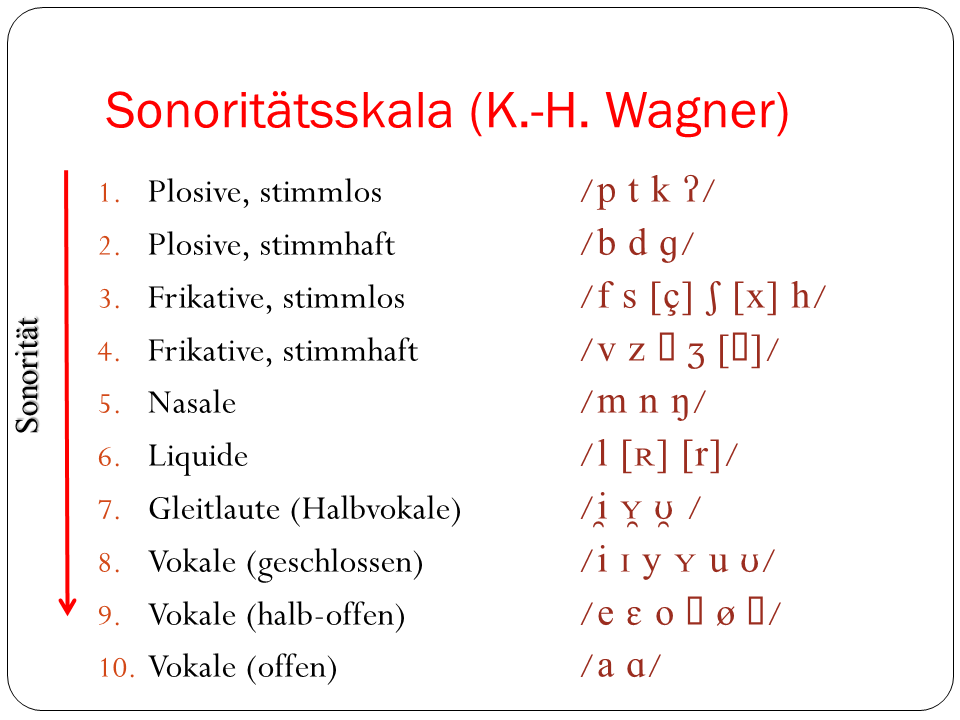
\includegraphics[width=1\textwidth,height=\textheight]{./pictures/Wagner_Maas_Duden_Petric_9.PNG}

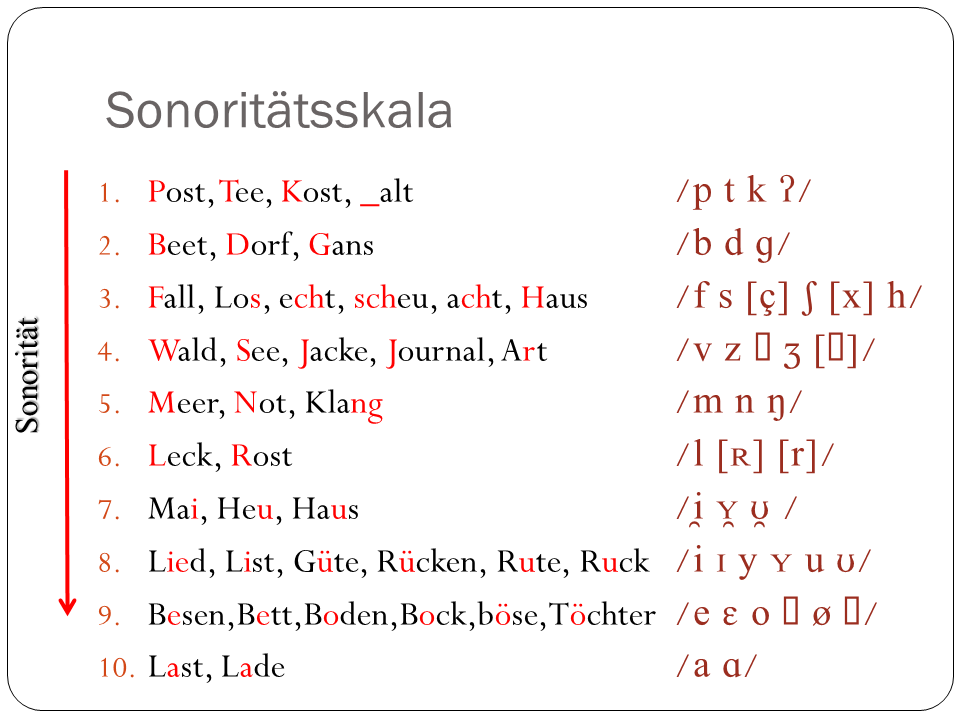
\includegraphics[width=1\textwidth,height=\textheight]{./pictures/Wagner_Maas_Duden_Petric_10.PNG}

Den Sonoritätsverlauf in einer Silbe oder Wortform kann man auch
graphisch darstellen:

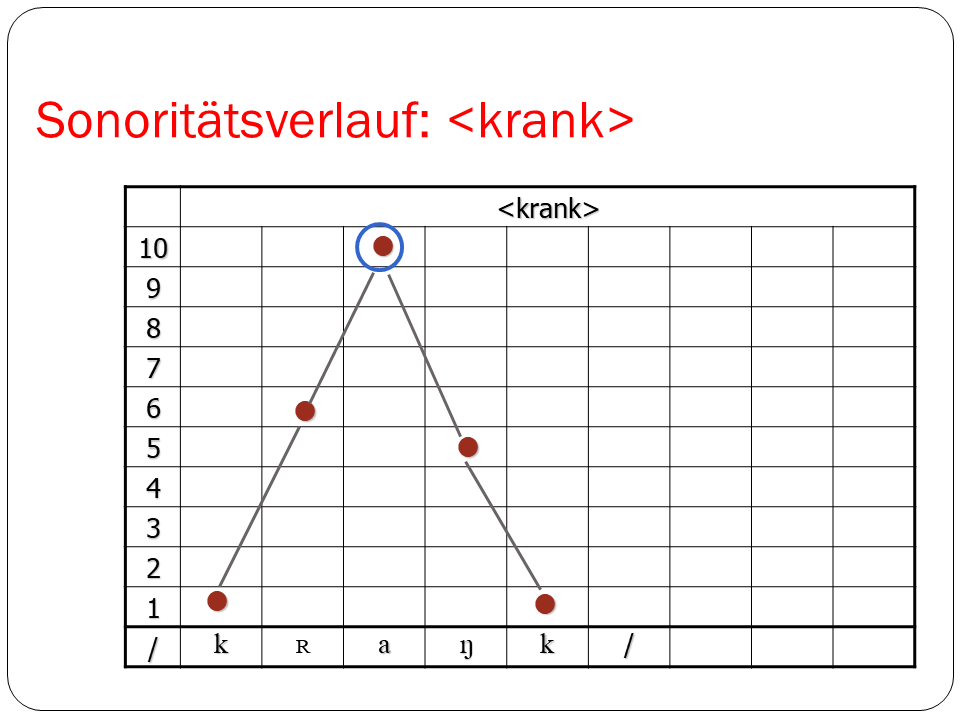
\includegraphics[width=1\textwidth,height=\textheight]{./pictures/Wagner_Maas_Duden_Petric_11.PNG}

Die Sonoritätsdistanz ist der Unterschied in der Wahrnehmbarkeit von
Lauten bzw. Lautklassen in einer Silbe. In den folgenden Beispielen wird
die Sonoritätsdistanz zwischen den jeweiligen Konsonanten im
Silbenanlaut (vor dem Vokal) berechnet, und zwar nach der
Sonoritätsskala von Wagner.

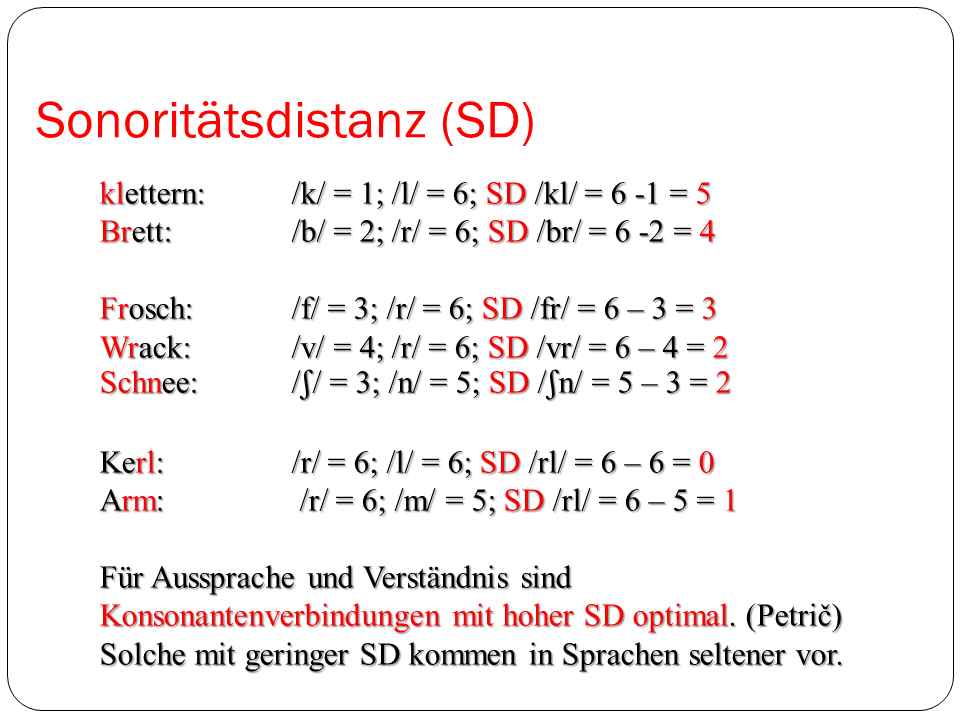
\includegraphics[width=1\textwidth,height=\textheight]{./pictures/Wagner_Maas_Duden_Petric_12.PNG}

\emph{Konsonantenverbindungen} sind allgemein perzeptuell und
artikulatorisch schwieriger als Einzelkonsonanten. Aber nicht alle
Konsonantenverbindungen sind gleich schwierig. \emph{Schwieriger}
scheinen Konsonantenverbindungen zu sein, wenn die \emph{Konsonanten
ähnlicher} sind, d.h. sich hinsichtlich ihrer Wahrnehmbarkeit nicht so
sehr unterscheiden. Das spielt auch eine Rolle im \emph{Spracherwerb},
z.B. auch im Fremdspracherwerb.

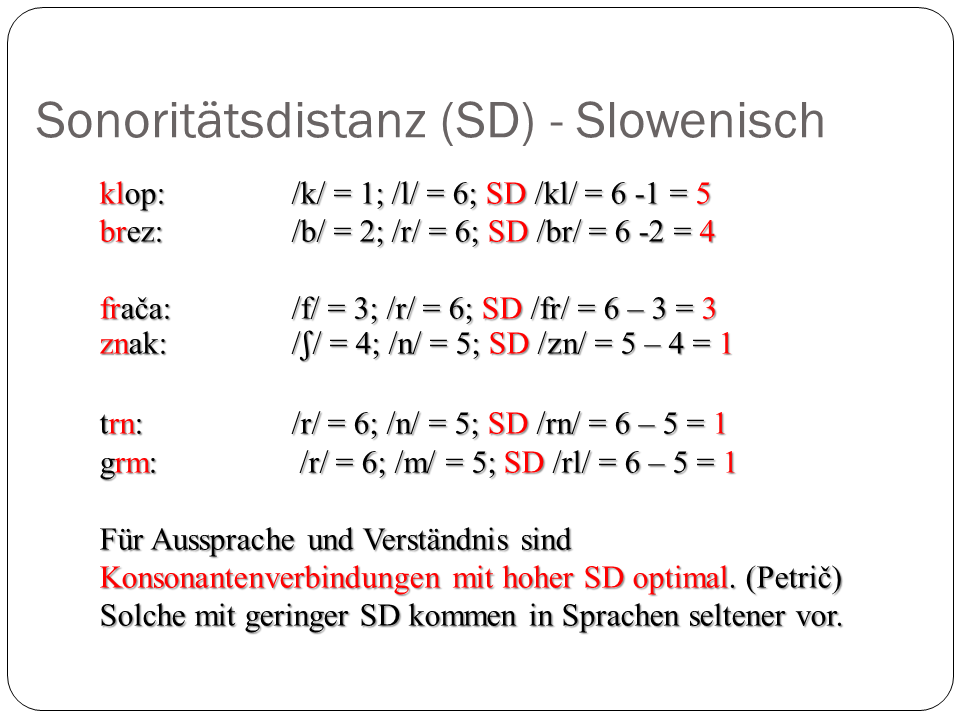
\includegraphics[width=1\textwidth,height=\textheight]{./pictures/Wagner_Maas_Duden_Petric_13.PNG}

\hypertarget{silbenaufbau}{%
\section{Silbenaufbau}\label{silbenaufbau}}

Dieses Kapitel enthält Darstellungen aus der Präsentation von Karl-Heinz
Wagner (Uni Bremen).

Eine heiß diskutierte Frage ist, ob Silben universell gesehen bzw.
einzelsprachlich gesehen \emph{hierarchisch oder flach strukturiert}
sind.

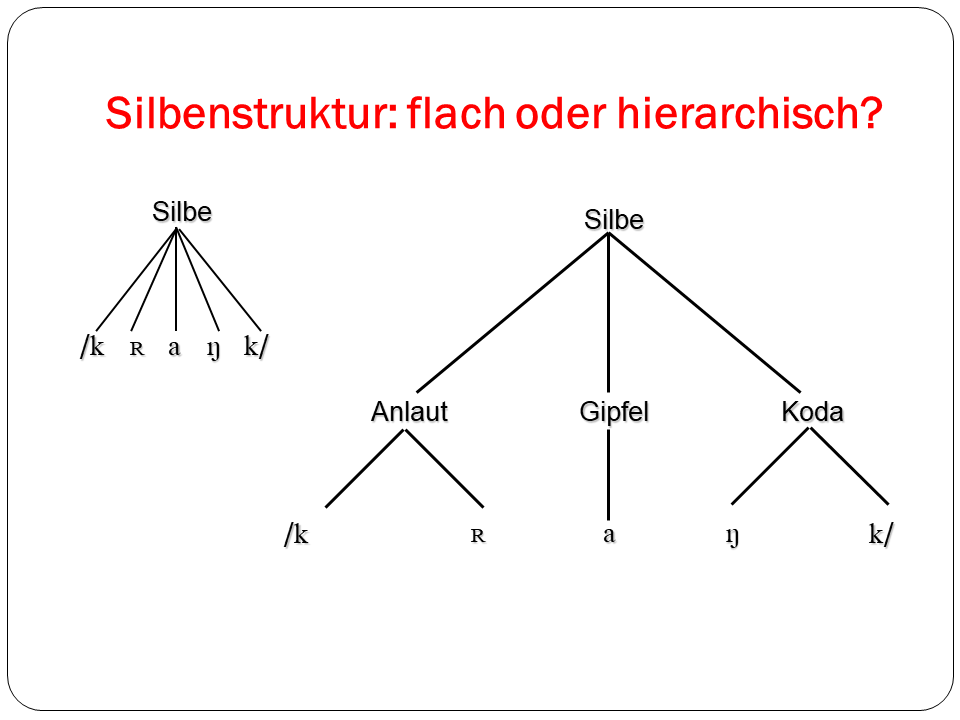
\includegraphics[width=1\textwidth,height=\textheight]{./pictures/Wagner_Maas_Duden_Petric_14.PNG}

Bei Befürwortung einer hierarchischen Silbenstruktur werden verschiedene
Bestandteile einer Silbe unterschieden. In der Forschung haben sich
verschiedene Bezeichnungen dafür etabliert:

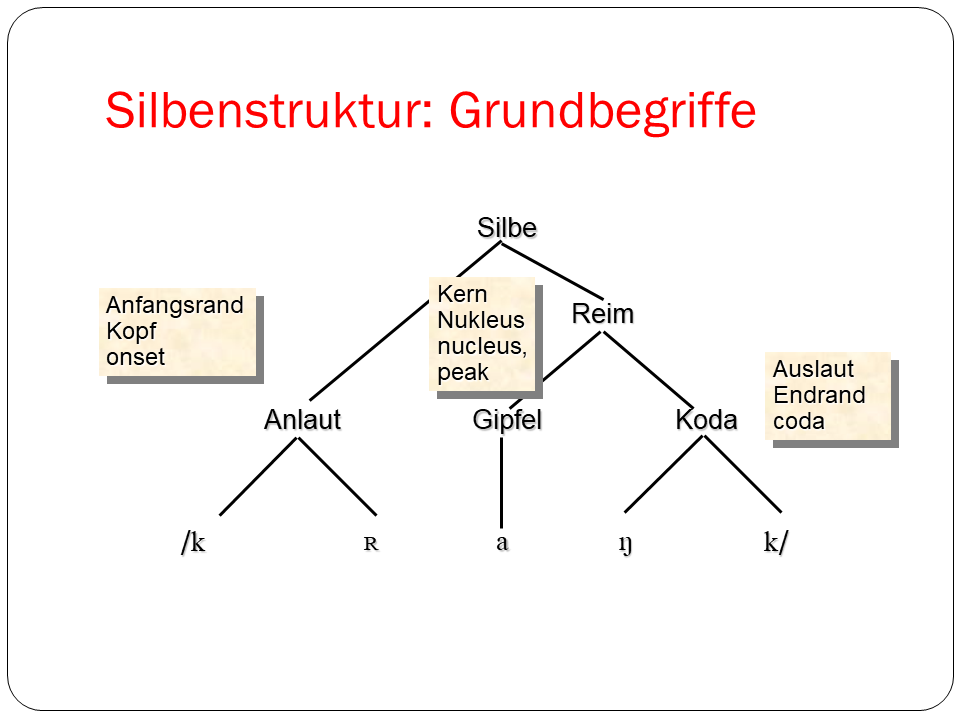
\includegraphics[width=1\textwidth,height=\textheight]{./pictures/Wagner_Maas_Duden_Petric_15.PNG}

Das hierarchische Strukturschema gibt Aufschluss darüber, dass zwischen
dem Silbenkern (Nukleus) und dem Silbenendrand engere Beziehungen
bestehen als zwischen Silbenanfangsrand und dem Nukleus.

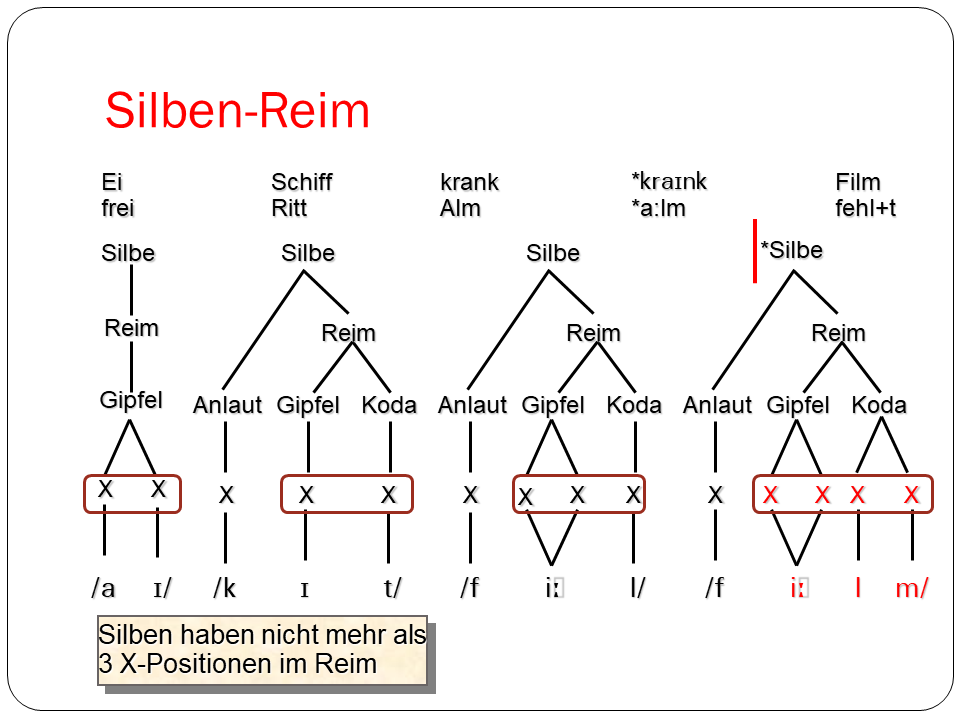
\includegraphics[width=1\textwidth,height=\textheight]{./pictures/Wagner_Maas_Duden_Petric_20.PNG}

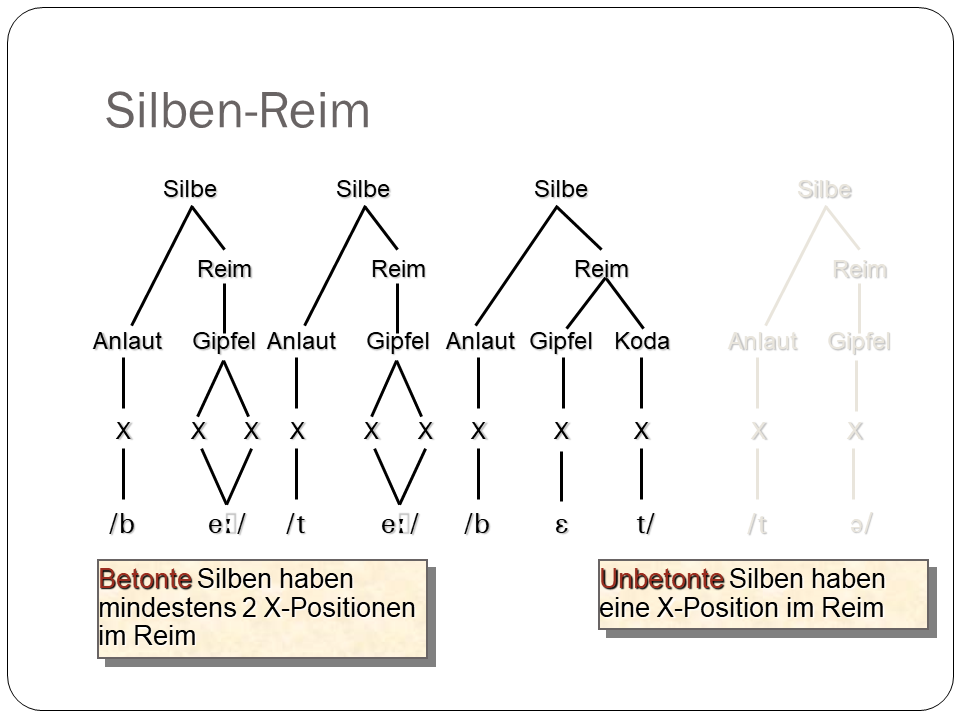
\includegraphics[width=1\textwidth,height=\textheight]{./pictures/Wagner_Maas_Duden_Petric_21.PNG}

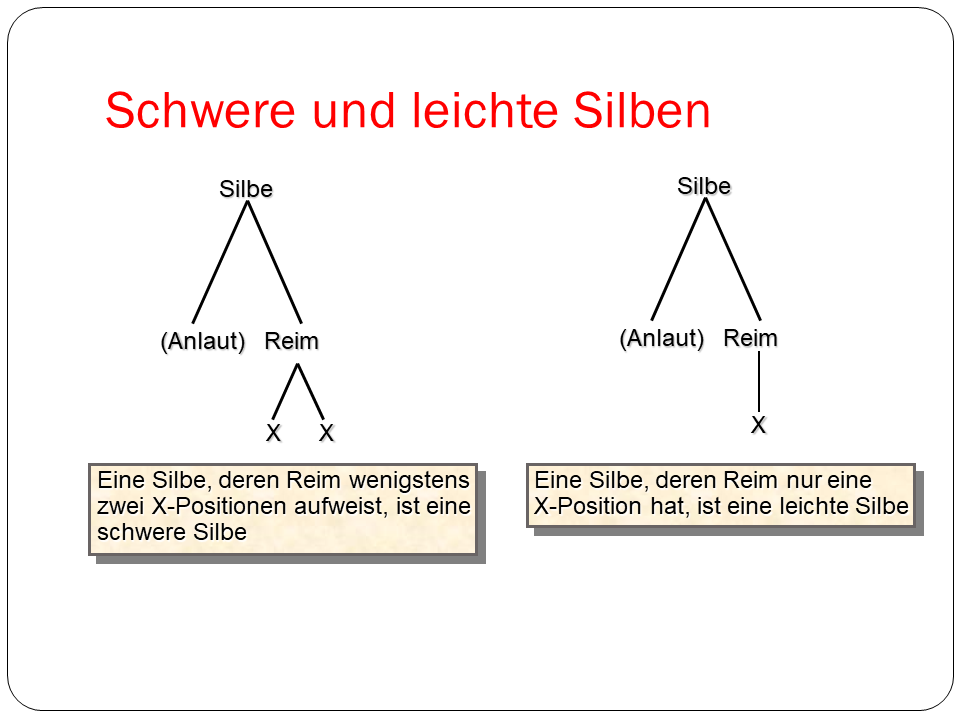
\includegraphics[width=1\textwidth,height=\textheight]{./pictures/Wagner_Maas_Duden_Petric_22.PNG}

Die Sonoritätshierarchie wird jedoch durch bestimmte
Konsonantenverbindungen verletzt. Ein Versuch, den Sonoritätsansatz zu
retten, ist die Einführung von außersilbischen Segmenten,
\emph{Appendizes}.

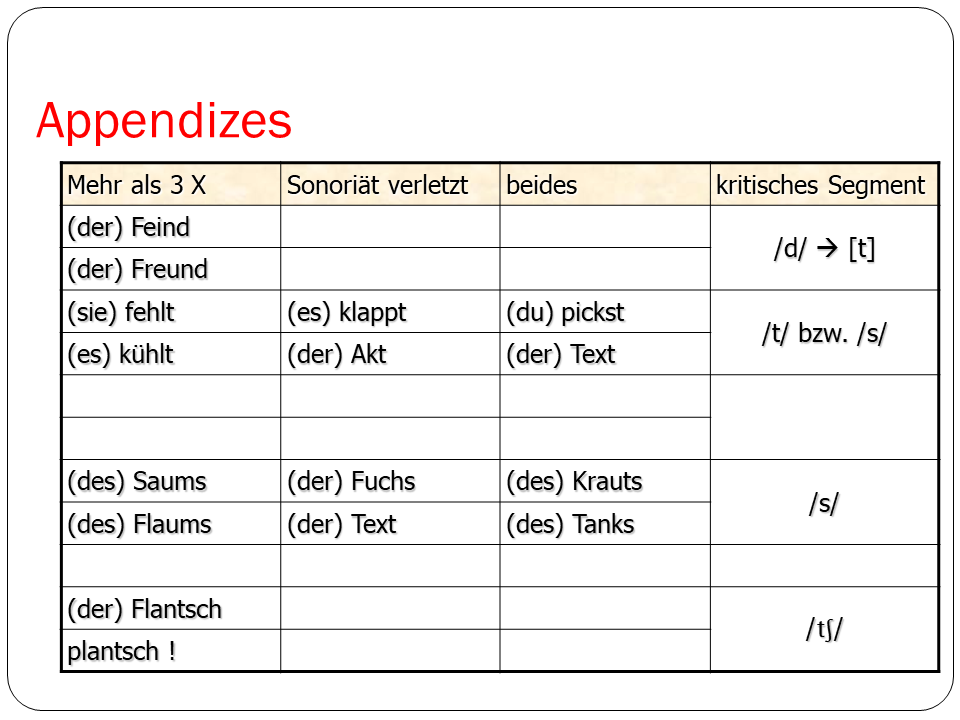
\includegraphics[width=1\textwidth,height=\textheight]{./pictures/Wagner_Maas_Duden_Petric_26.PNG}

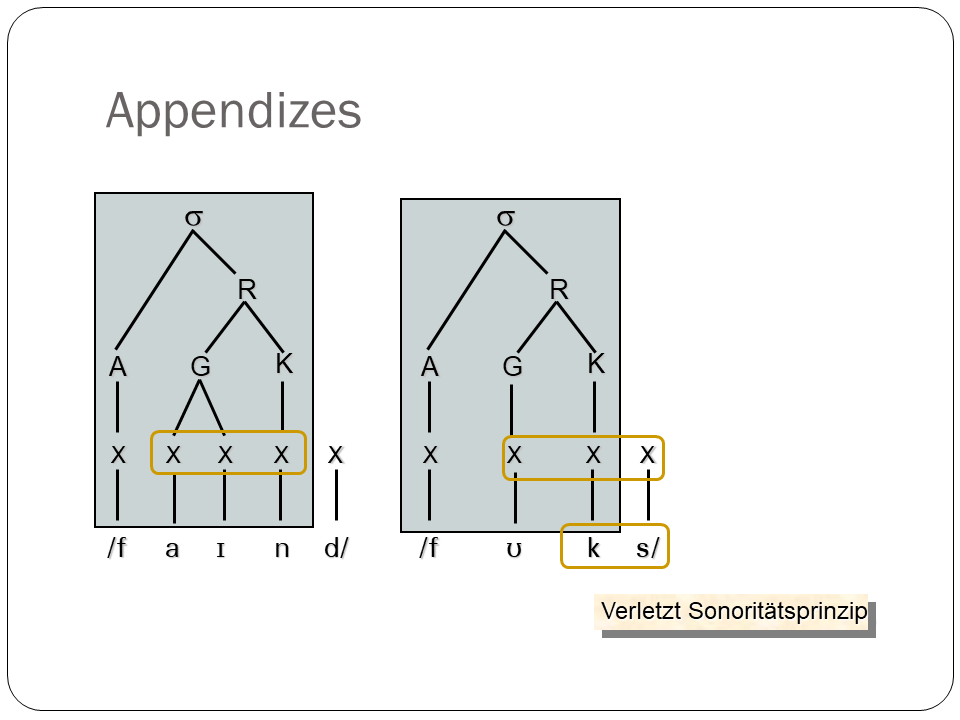
\includegraphics[width=1\textwidth,height=\textheight]{./pictures/Wagner_Maas_Duden_Petric_27.PNG}

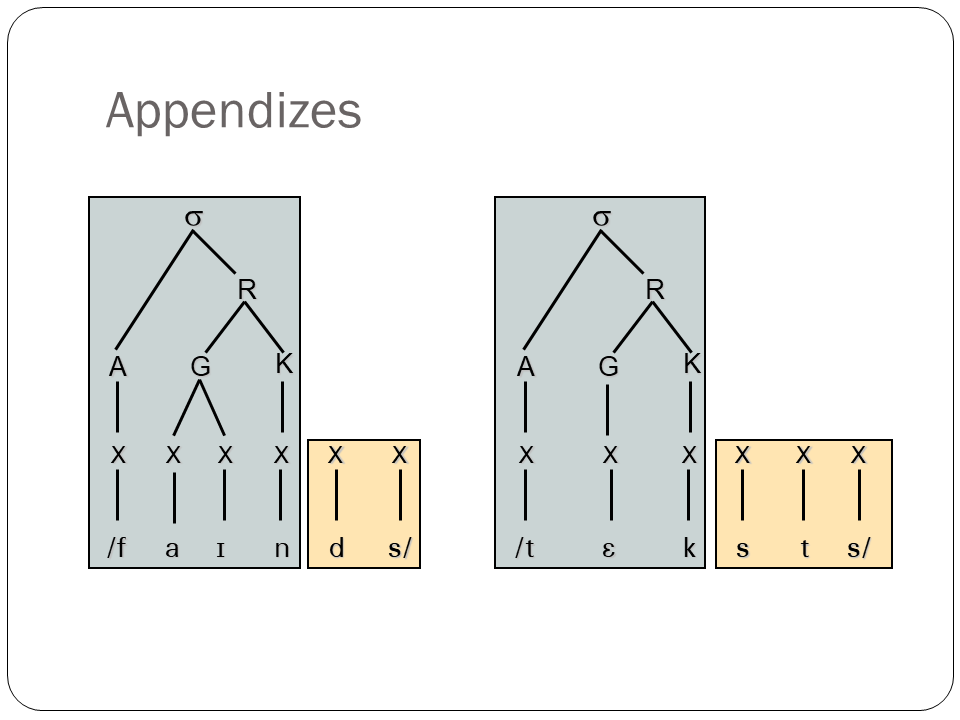
\includegraphics[width=1\textwidth,height=\textheight]{./pictures/Wagner_Maas_Duden_Petric_28.PNG}

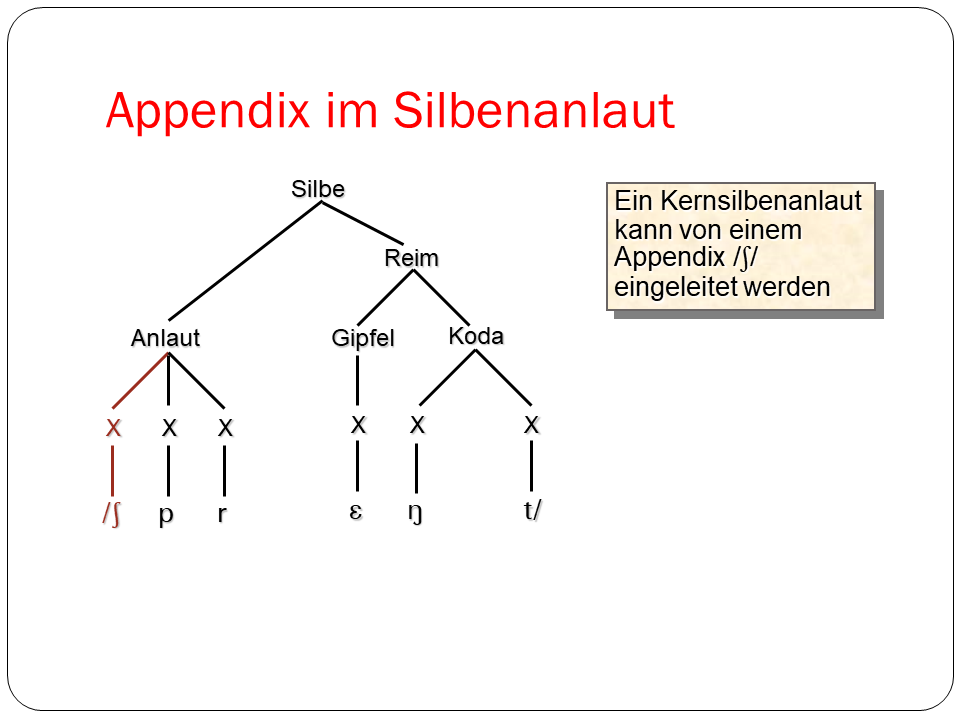
\includegraphics[width=1\textwidth,height=\textheight]{./pictures/Wagner_Maas_Duden_Petric_29.PNG}

Ambisyllabische Konsonanten oder Silbengelenke als ein weiteres Problem
bei der Zuordnung zu Silben:

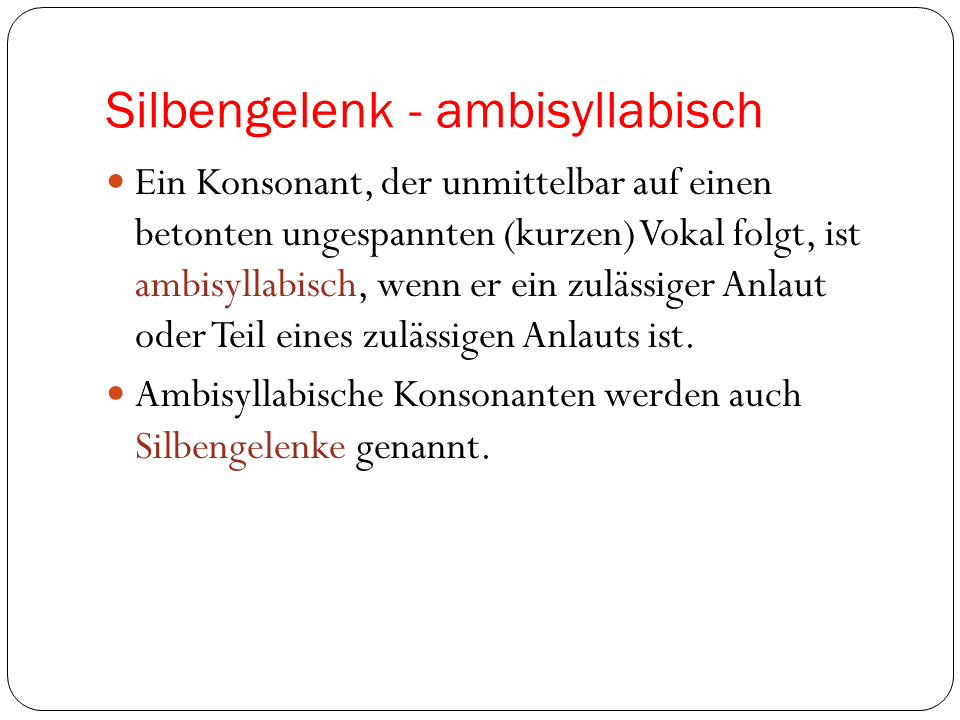
\includegraphics[width=1\textwidth,height=\textheight]{./pictures/Wagner_Maas_Duden_Petric_39.PNG}

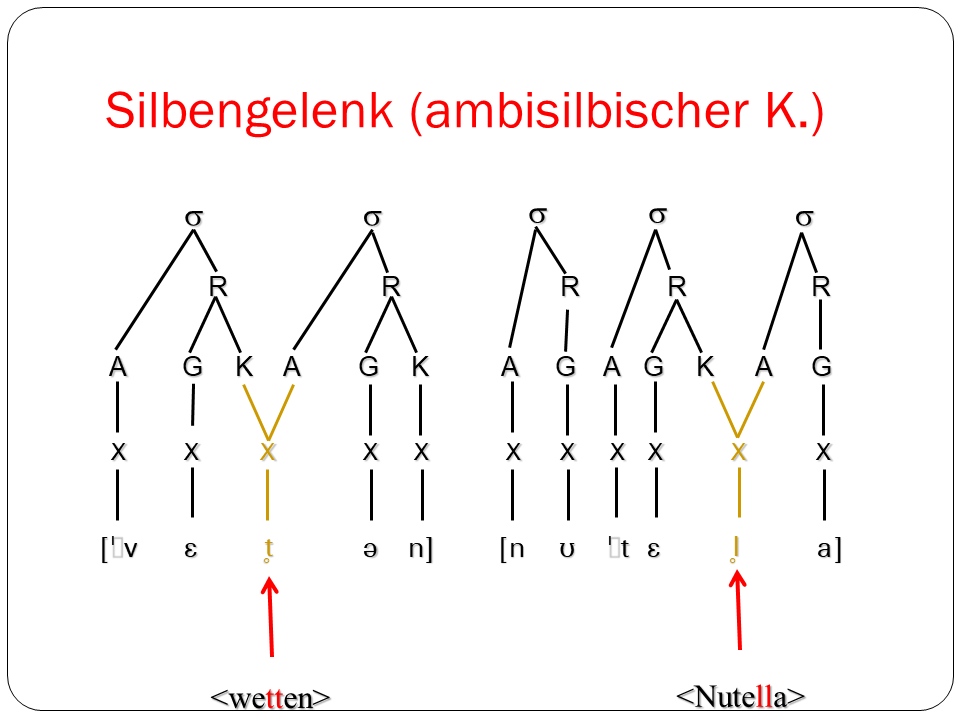
\includegraphics[width=1\textwidth,height=\textheight]{./pictures/Wagner_Maas_Duden_Petric_40.PNG}

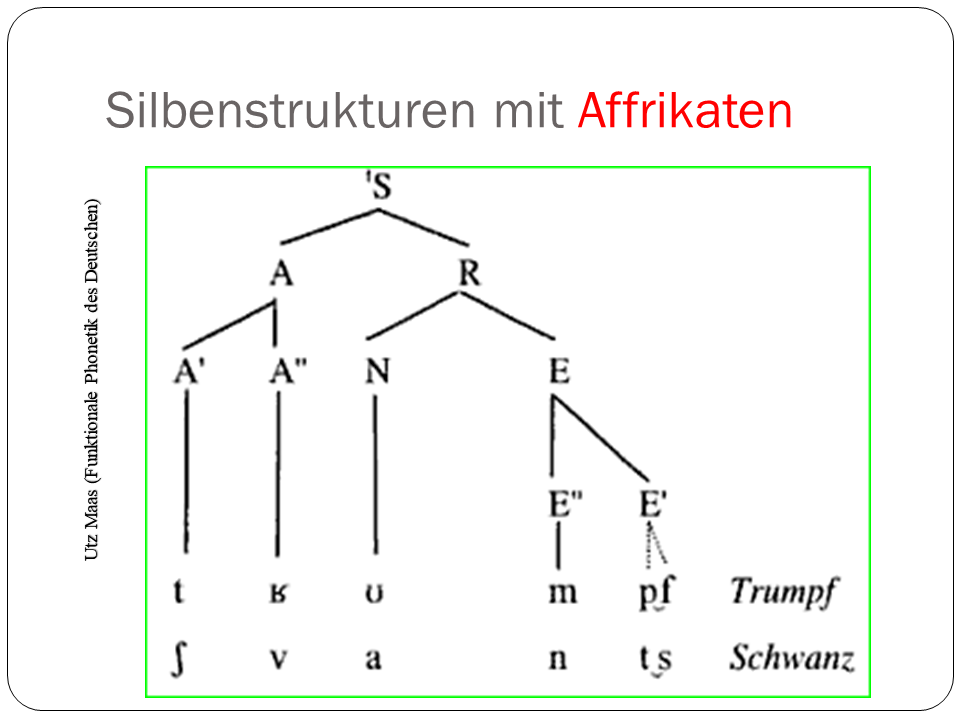
\includegraphics[width=1\textwidth,height=\textheight]{./pictures/Wagner_Maas_Duden_Petric_41.PNG}

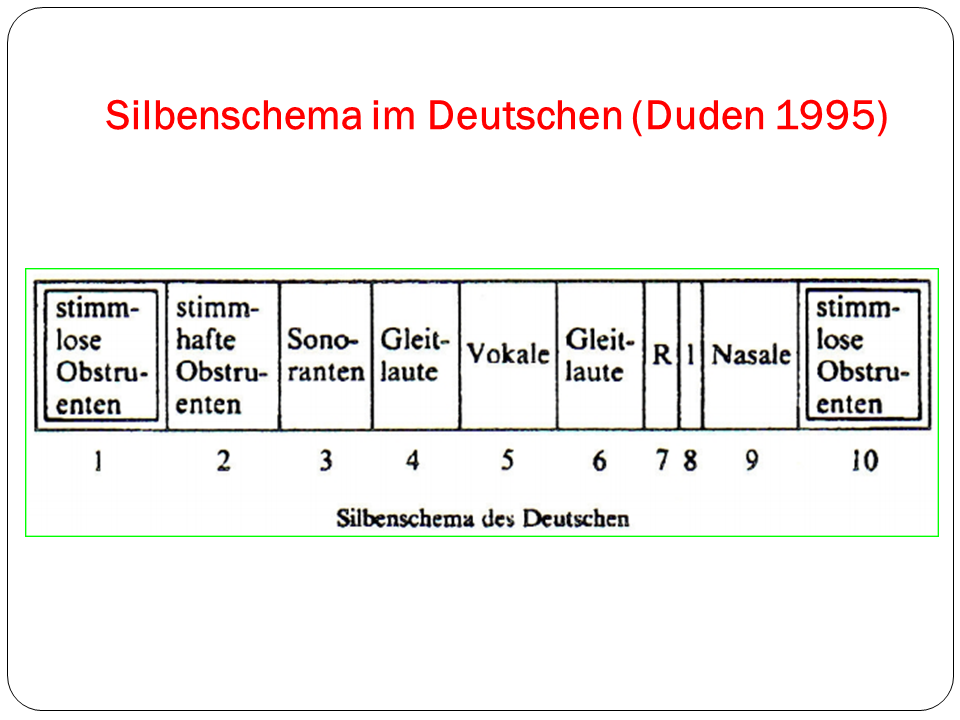
\includegraphics[width=1\textwidth,height=\textheight]{./pictures/Wagner_Maas_Duden_Petric_42.PNG}

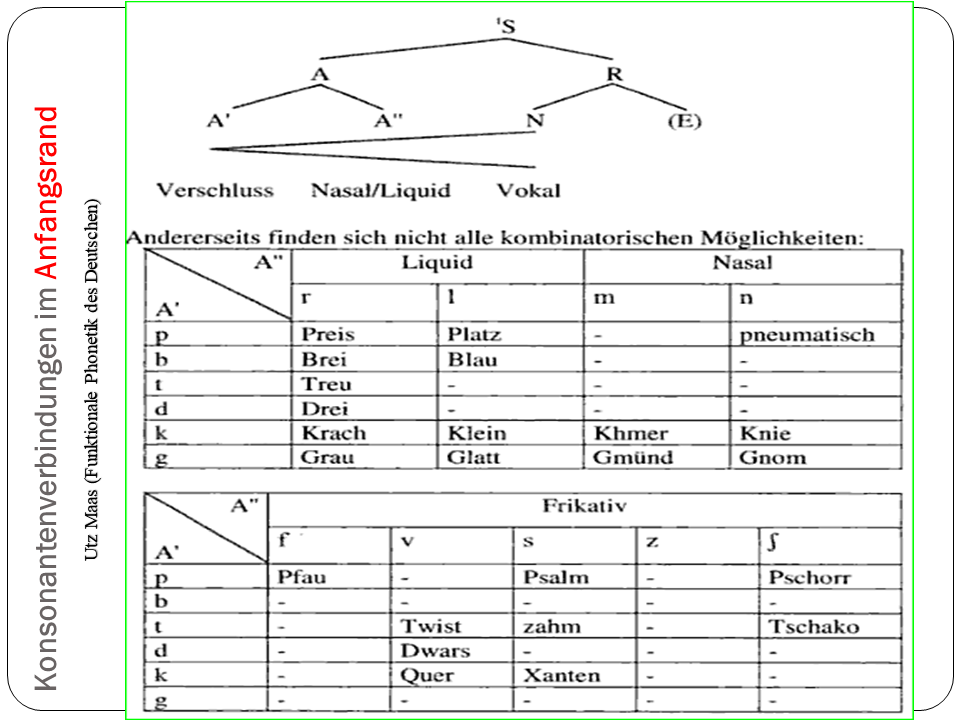
\includegraphics[width=1\textwidth,height=\textheight]{./pictures/Wagner_Maas_Duden_Petric_43.PNG}

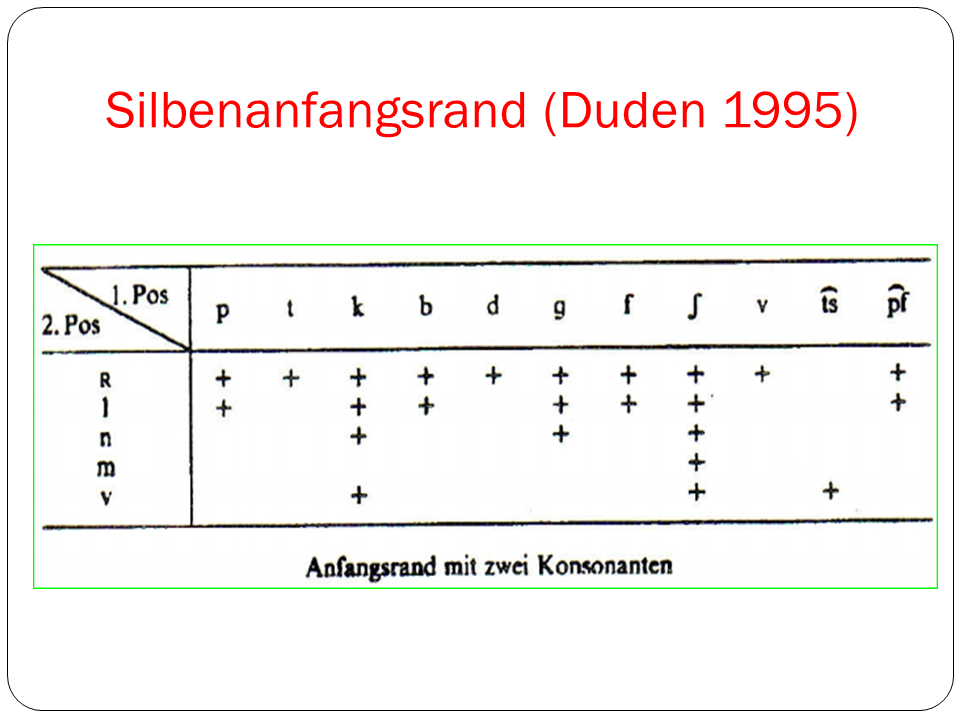
\includegraphics[width=1\textwidth,height=\textheight]{./pictures/Wagner_Maas_Duden_Petric_44.PNG}

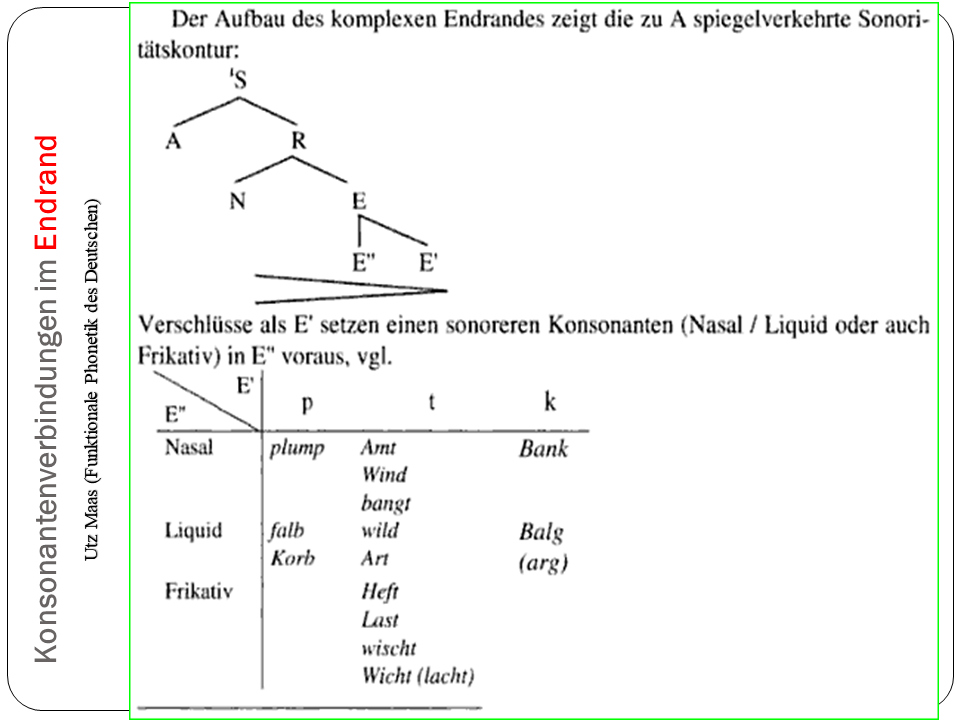
\includegraphics[width=1\textwidth,height=\textheight]{./pictures/Wagner_Maas_Duden_Petric_45.PNG}

\includegraphics[width=1\textwidth,height=\textheight]{./pictures/Wagner_Maas_Duden_Petric_46.PNG}

\includegraphics[width=1\textwidth,height=\textheight]{./pictures/Wagner_Maas_Duden_Petric_47.PNG}

\includegraphics[width=1\textwidth,height=\textheight]{./pictures/Wagner_Maas_Duden_Petric_48.PNG}

\includegraphics[width=1\textwidth,height=\textheight]{./pictures/Wagner_Maas_Duden_Petric_49.PNG}

\includegraphics[width=1\textwidth,height=\textheight]{./pictures/Wagner_Maas_Duden_Petric_50.PNG}

\hypertarget{silbengrenze}{%
\section{Silbengrenze}\label{silbengrenze}}

\includegraphics[width=1\textwidth,height=\textheight]{./pictures/Wagner_Maas_Duden_Petric_24.PNG}

\includegraphics[width=1\textwidth,height=\textheight]{./pictures/Wagner_Maas_Duden_Petric_25.PNG}

\includegraphics[width=1\textwidth,height=\textheight]{./pictures/04_Die_Lage_der_Silbengrenze_page-0001.jpg}

\hypertarget{phonologische-prozesse}{%
\chapter{Phonologische Prozesse}\label{phonologische-prozesse}}

\hypertarget{prosodie-1}{%
\chapter{Prosodie}\label{prosodie-1}}

\part{Aussprachepraxis im Sprachlabor}

\hypertarget{wortakzentuierung-sec-wortakzent}{%
\chapter{Wortakzentuierung
{[}\#sec-wortakzent{]}}\label{wortakzentuierung-sec-wortakzent}}

\hypertarget{akzentuierung-von-phrasen-sec-satzakzent}{%
\chapter{Akzentuierung von Phrasen
{[}\#sec-satzakzent{]}}\label{akzentuierung-von-phrasen-sec-satzakzent}}

\hypertarget{melodiebewegungen-in-uxe4uuxdferungen-sec-satzmelodie}{%
\chapter{Melodiebewegungen in Äußerungen
{[}\#sec-satzmelodie{]}}\label{melodiebewegungen-in-uxe4uuxdferungen-sec-satzmelodie}}

\hypertarget{vokale-im-einzelnen-sec-vokale}{%
\chapter{Vokale im Einzelnen
{[}\#sec-vokale{]}}\label{vokale-im-einzelnen-sec-vokale}}

\hypertarget{konsonanten-im-einzelnen-sec-konsonanten}{%
\chapter{Konsonanten im Einzelnen
{[}\#sec-konsonanten{]}}\label{konsonanten-im-einzelnen-sec-konsonanten}}

\bookmarksetup{startatroot}

\hypertarget{summary}{%
\chapter{Summary}\label{summary}}

In summary, this book has no content whatsoever.

\begin{verbatim}
[1] 2
\end{verbatim}

\bookmarksetup{startatroot}

\hypertarget{references}{%
\chapter*{References}\label{references}}
\addcontentsline{toc}{chapter}{References}

\markboth{References}{References}

\hypertarget{refs}{}
\begin{CSLReferences}{1}{0}
\leavevmode\vadjust pre{\hypertarget{ref-bussmann1990lexikon}{}}%
Bußmann, Hadumod. 1990. {``Lexikon Der Sprachwissenschaft.''}

\leavevmode\vadjust pre{\hypertarget{ref-drosdowski1995duden}{}}%
Drosdowski, Günther. 1995. \emph{Duden" Grammatik Der Deutschen
Gegenwartssprache"}. Bibliograph. Institut.

\leavevmode\vadjust pre{\hypertarget{ref-engel2008deutsche}{}}%
Engel, Ulrich. 2008. \emph{Deutsche Grammatik}.

\leavevmode\vadjust pre{\hypertarget{ref-grebe1973duden}{}}%
Grebe, Paul, and Helmut Gipper. 1973. \emph{Duden" Grammatik Der
Deutschen Gegenwartssprache"}. Bibliograph. Institut.

\leavevmode\vadjust pre{\hypertarget{ref-gross1990linguistik}{}}%
Gross, Harro. 1990. \emph{Einf{ü}hrung in Die Germanistische
Linguistik}. iudicium.

\leavevmode\vadjust pre{\hypertarget{ref-neppert1992elemente}{}}%
Neppert, Joachim, and Magnús Pétursson. 1992. \emph{Elemente Einer
Akustischen Phonetik}. Buske Hamburg.

\leavevmode\vadjust pre{\hypertarget{ref-toporivsivc1992slovenska}{}}%
Toporišič, Jože. 1992. \emph{Slovenska Slovnica}. Obzorja.

\end{CSLReferences}


\backmatter

\printindex

\end{document}
